\singlespacing
\chapter{Diseño, construcción y aplicación de un microespectrómetro}
\label{chap:microsp}
\spacing{1.5}

\hspace{0.5cm}En el Capítulo \ref{chap:zeiss} se realizó un análisis cuantitativo de los defectos de filtros multiespectrales de cámaras de satélites: se determinó su área, su diámetro equivalente, etcétera. Dicho análisis permitió aplicar las especificaciones técnicas de \textit{scratch \& dig} y de la ISO 10110, lo que resulta fundamental para establecer las bases de futuros acuerdos con los fabricantes de los componentes ópticos. Al mismo tiempo, los resultados de la población de defectos [\ref{sec:defpob}] detectados con el algoritmo, permitieron establecer los criterios de diseño óptico del microespectrómetro que se explica en el presente capítulo.

Como se explicó en la Sección \ref{sec:microespp}, un microespectrómetro es un instrumento de medición híbrido que integra la capacidad de magnificación y de resolución ópticas de un microscopio con la capacidad de inferir las propiedades espectrales de un material. En este capítulo se describe el diseño y la construcción de un microespectrómetro que permitió realizar una caracterización del filtro y de sus defectos a través de los espectros de transmisión.
%%%%%%%%%%%%%%%%%%%%%%%%%%%%%%%%%%%%%%%%%%%%%%%%%%%%%%%%%%%%%%%%%%%%%%%%%%%%%%%%%%%%%%%%%%%%%%%%%%%%%%%%%%%%%%%%%%%%%%%%%%%%%%%%%%%%%%%%%%%%%%%%%%%%%%%%%%%%%%%%%%%%%%%%%%%%%%%%%%%%%%%%%%%%%%%%%%%%%%%%%%%%%%%%%%%%%%%%%%%%

\singlespacing
\section{Prototipo preliminar \href{https://github.com/jrr1984/Prototipo0\_S-D\_SpectralGUI}{\faGithub$_{3.1}$}}
\label{sec:prot0}
\spacing{1.5}

\hspace{0.5cm}El desarrollo del prototipo preliminar que se muestra en esta sección permitió establecer los criterios de elección de la fuente de luz y el recorrido y la precisión necesarias de la platina desarrollada para poder adquirir el espectro e imágenes del filtro completo. Como buena práctica de prototipado de instrumentos de medición se utilizaron componentes y equipamiento disponibles en el laboratorio, es decir que no se incurrió en gastos adicionales de dinero a excepción del costo del material de las impresiones 3D del soporte del filtro. Por otro lado, a partir del desarrollo del software automatizado de adquisición y de visualización de los resultados de este prototipo se establecieron las características deseadas y esperadas del prototipo final desarrollado. De esta manera, el prototipo permitió establecer la factibilidad del desarrollo del equipo.

Como objetivo general se propuso desarrollar un sistema integral de caracterización de filtros ópticos de interferencia utilizados en cámaras hiper y multiespectrales. Inicialmente se establecieron tres objetivos específicos:
\begin{enumerate}
\item Desarrollar un sistema automatizado de adquisición del espectro de transmisión de cada una de las bandas del filtro [\href{https://github.com/jrr1984/Prototipo0\_S-D\_SpectralGUI/blob/master/barrido/std}{\faGithub$_{3.1.1}$}].

\item Determinar un mapa multiespectral ($\textit{x}$,$\textit{y}$,$\lambda$) del filtro [\href{https://github.com/jrr1984/Prototipo0\_S-D\_SpectralGUI/blob/master/spectral\_gui/main.py}{\faGithub$_{3.1.2}$}].

\item Integrar un sistema de detección y caracterización de los defectos del filtro.
\end{enumerate}

A continuación se describen los primeros dos objetivos que fueron abarcados por el prototipo preliminar descripto en esta sección. Respecto del primer objetivo, se montó el arreglo experimental que se muestra en las Figuras \ref{fig:p} (a), (b) y (c). 

Con una fuente de luz halógena, modelo \href{https://dolan-jenner.com/products/fiber-lite-190}{\textit{Fiber-lite 190 Illuminator}}, se incidió perpendicularmente sobre el filtro y su transmisión fue detectada por la fibra óptica de un espectrómetro modelo \href{https://www.thorlabs.com/thorproduct.cfm?partnumber=CCS200/M#ad-image-0}{CCS 200/M} de la empresa Thorlabs (\textit{Driver} de \textit{python}: \href{https://github.com/jrr1984/Prototipo0\_S-D\_SpectralGUI/blob/master/syst/CCS200.py}{\faGithub$_{3.1.3}$}). De la misma manera en que se realizó el \textit{Tile Scan} del filtro completo con el microscopio Zeiss explicado en la sección \ref{subs:tilsc} (Ver Figura \ref{fig:tilescan}), se desplazó el filtro a lo largo del eje x, barriendo en `filas' y realizando el desplazamiento vertical en los extremos del máximo recorrido de los tornillos accionados por los motores paso a paso que fue de 13 mm. Dicho desplazamiento fue realizado con una plataforma de tres grados de libertad, modelo \href{https://www.thorlabs.com/thorproduct.cfm?partnumber=MT3/M}{MT3/M} de la empresa Thorlabs, cuyos tornillos micrométricos fueron intercambiados por unos motores paso a paso modelo \href{https://www.thorlabs.com/thorproduct.cfm?partnumber=ZST213B}{ZST213B} cuyos controladores de corriente fueron también de la empresa Thorlabs, modelo \href{https://www.thorlabs.com/thorproduct.cfm?partnumber=KST101}{KST101} (\textit{Driver} de \textit{python}: \href{https://github.com/jrr1984/Prototipo0\_S-D\_SpectralGUI/blob/master/barrido/std/thor\_stepm.py}{\faGithub$_{3.1.4}$}). Como las dimensiones de la región comprendida por las cinco bandas del filtro es de 27 mm x 25 mm, con esta plataforma no se pudo realizar una adquisición del filtro completa en una sola configuración como la propuesta. El \textit{software} automatizado de adquisición del espectro de transmisión del filtro desarrollado para este prototipo [\href{https://github.com/jrr1984/Prototipo0\_S-D\_SpectralGUI/tree/master/barrido/std}{\faGithub$_{3.1.1}$}] fue expandido en el prototipo final y se lo explica en la Sección \ref{sec:softadq}.

\begin{figure}[H]
%\centering
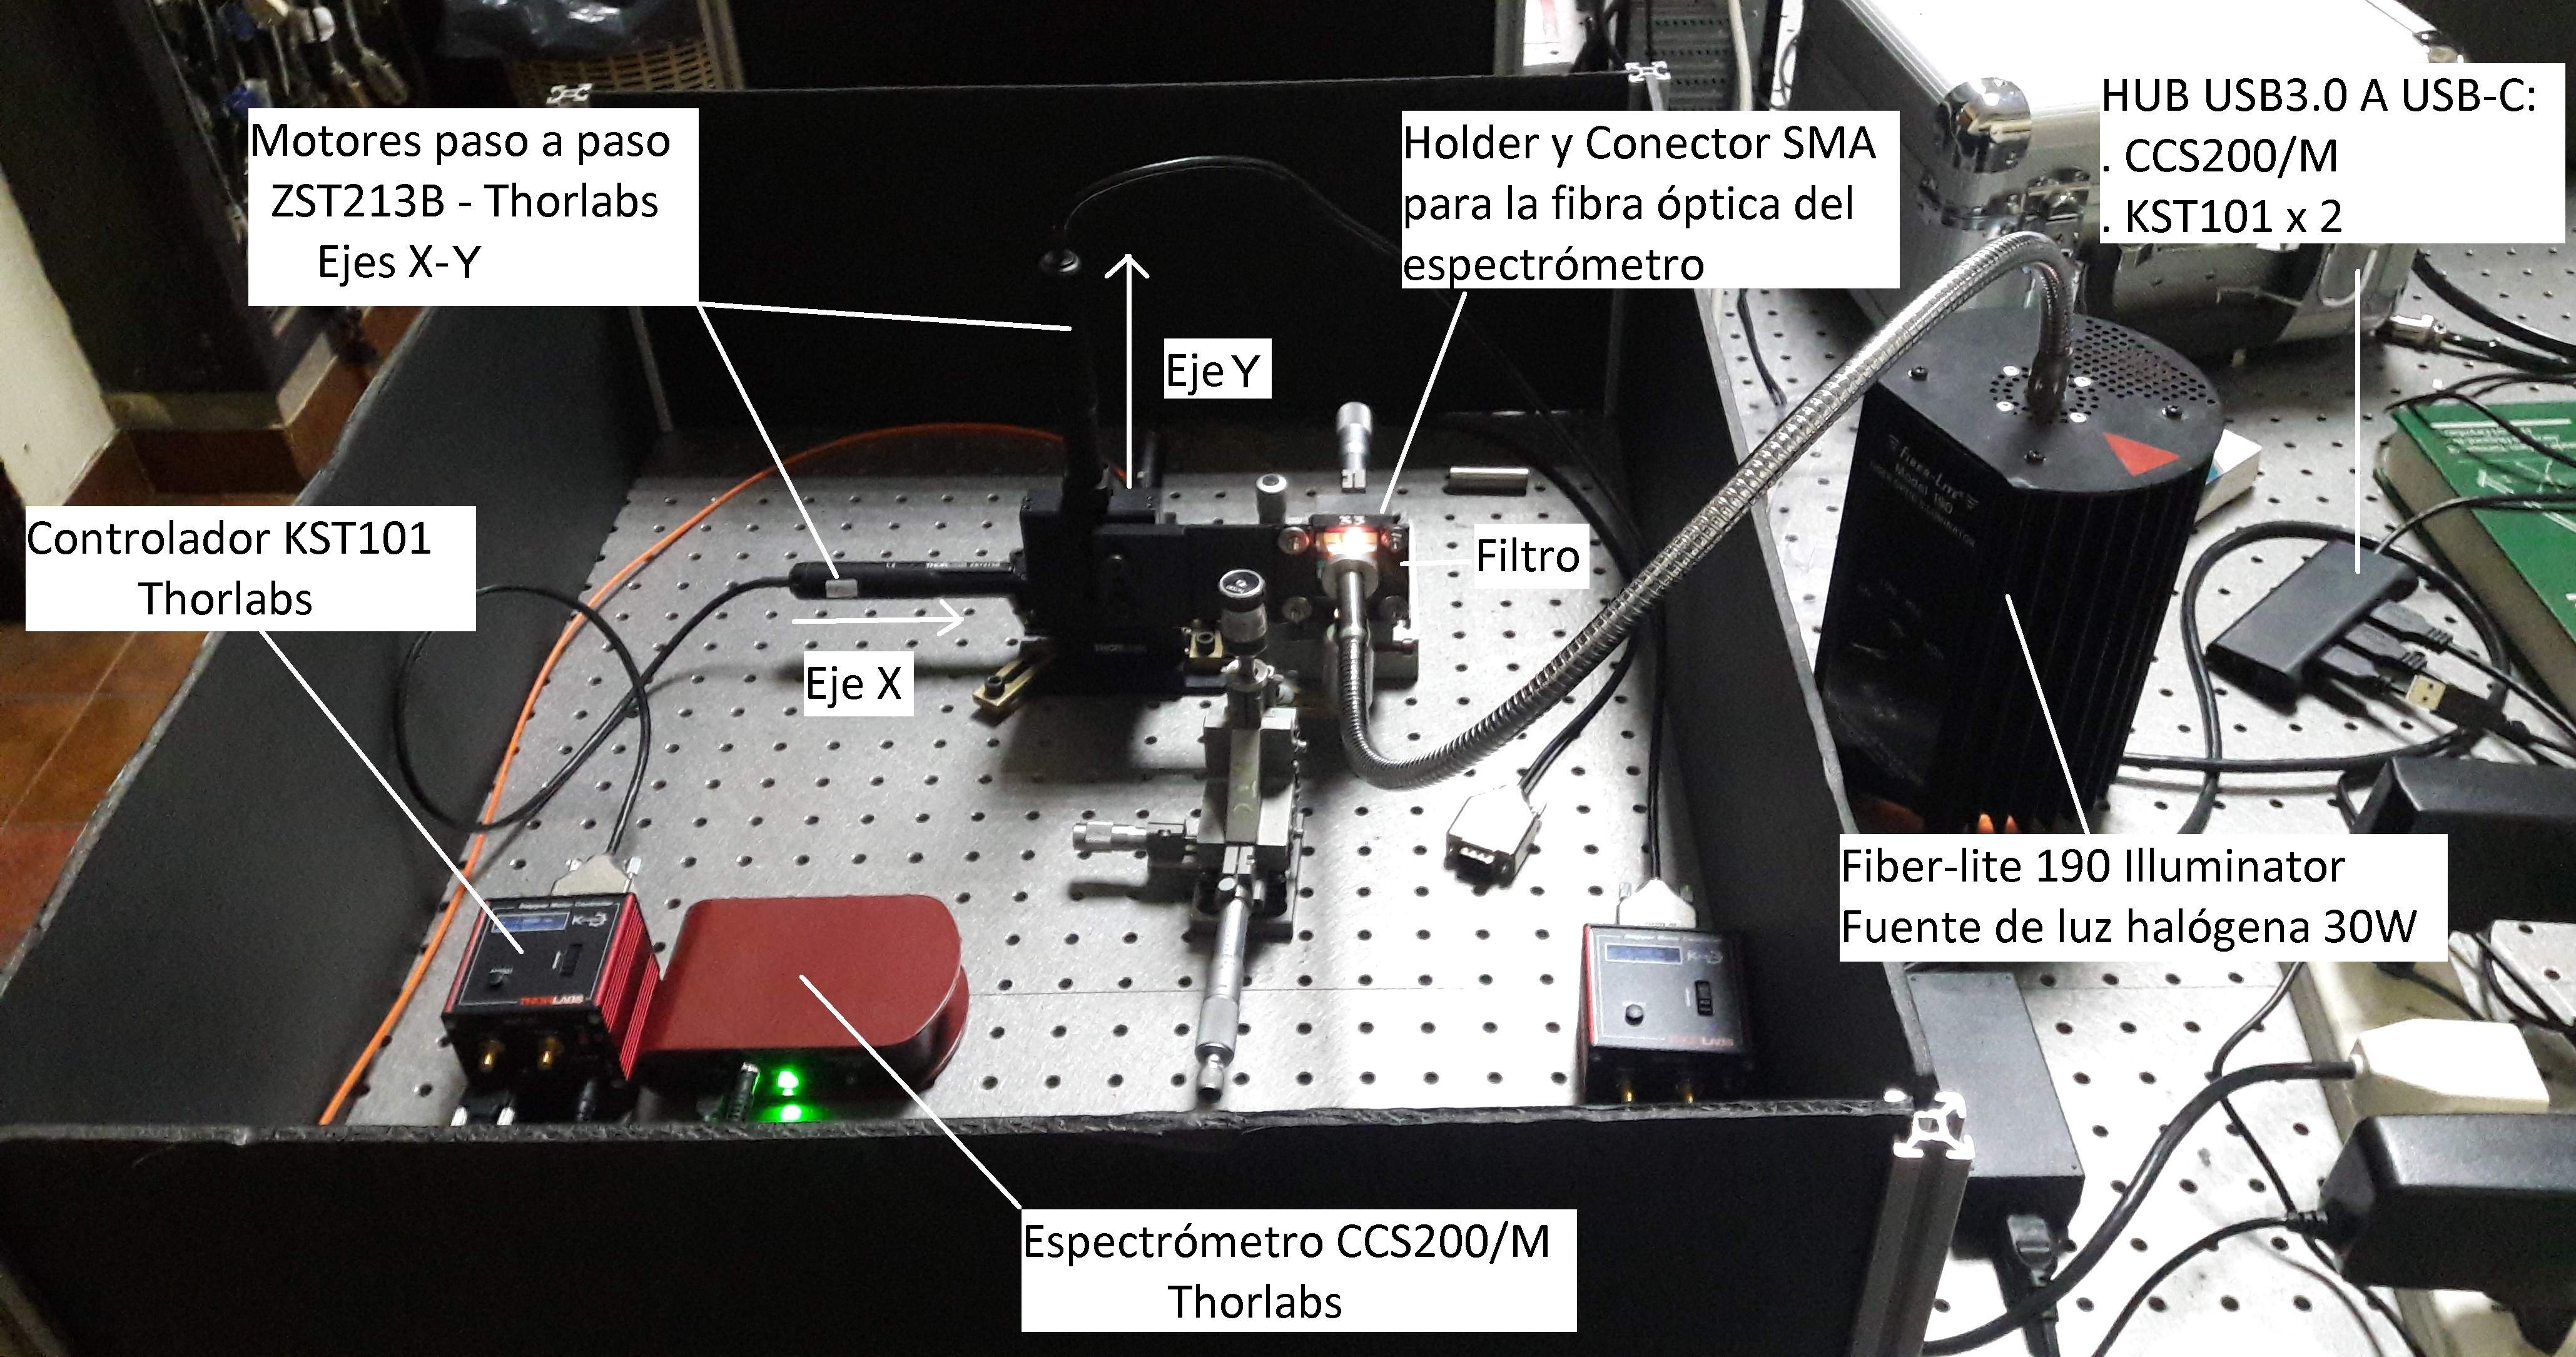
\includegraphics[width=1.0\textwidth]{Figs/microespectrometro/setupbarridooriginal.jpg}
\hfill%
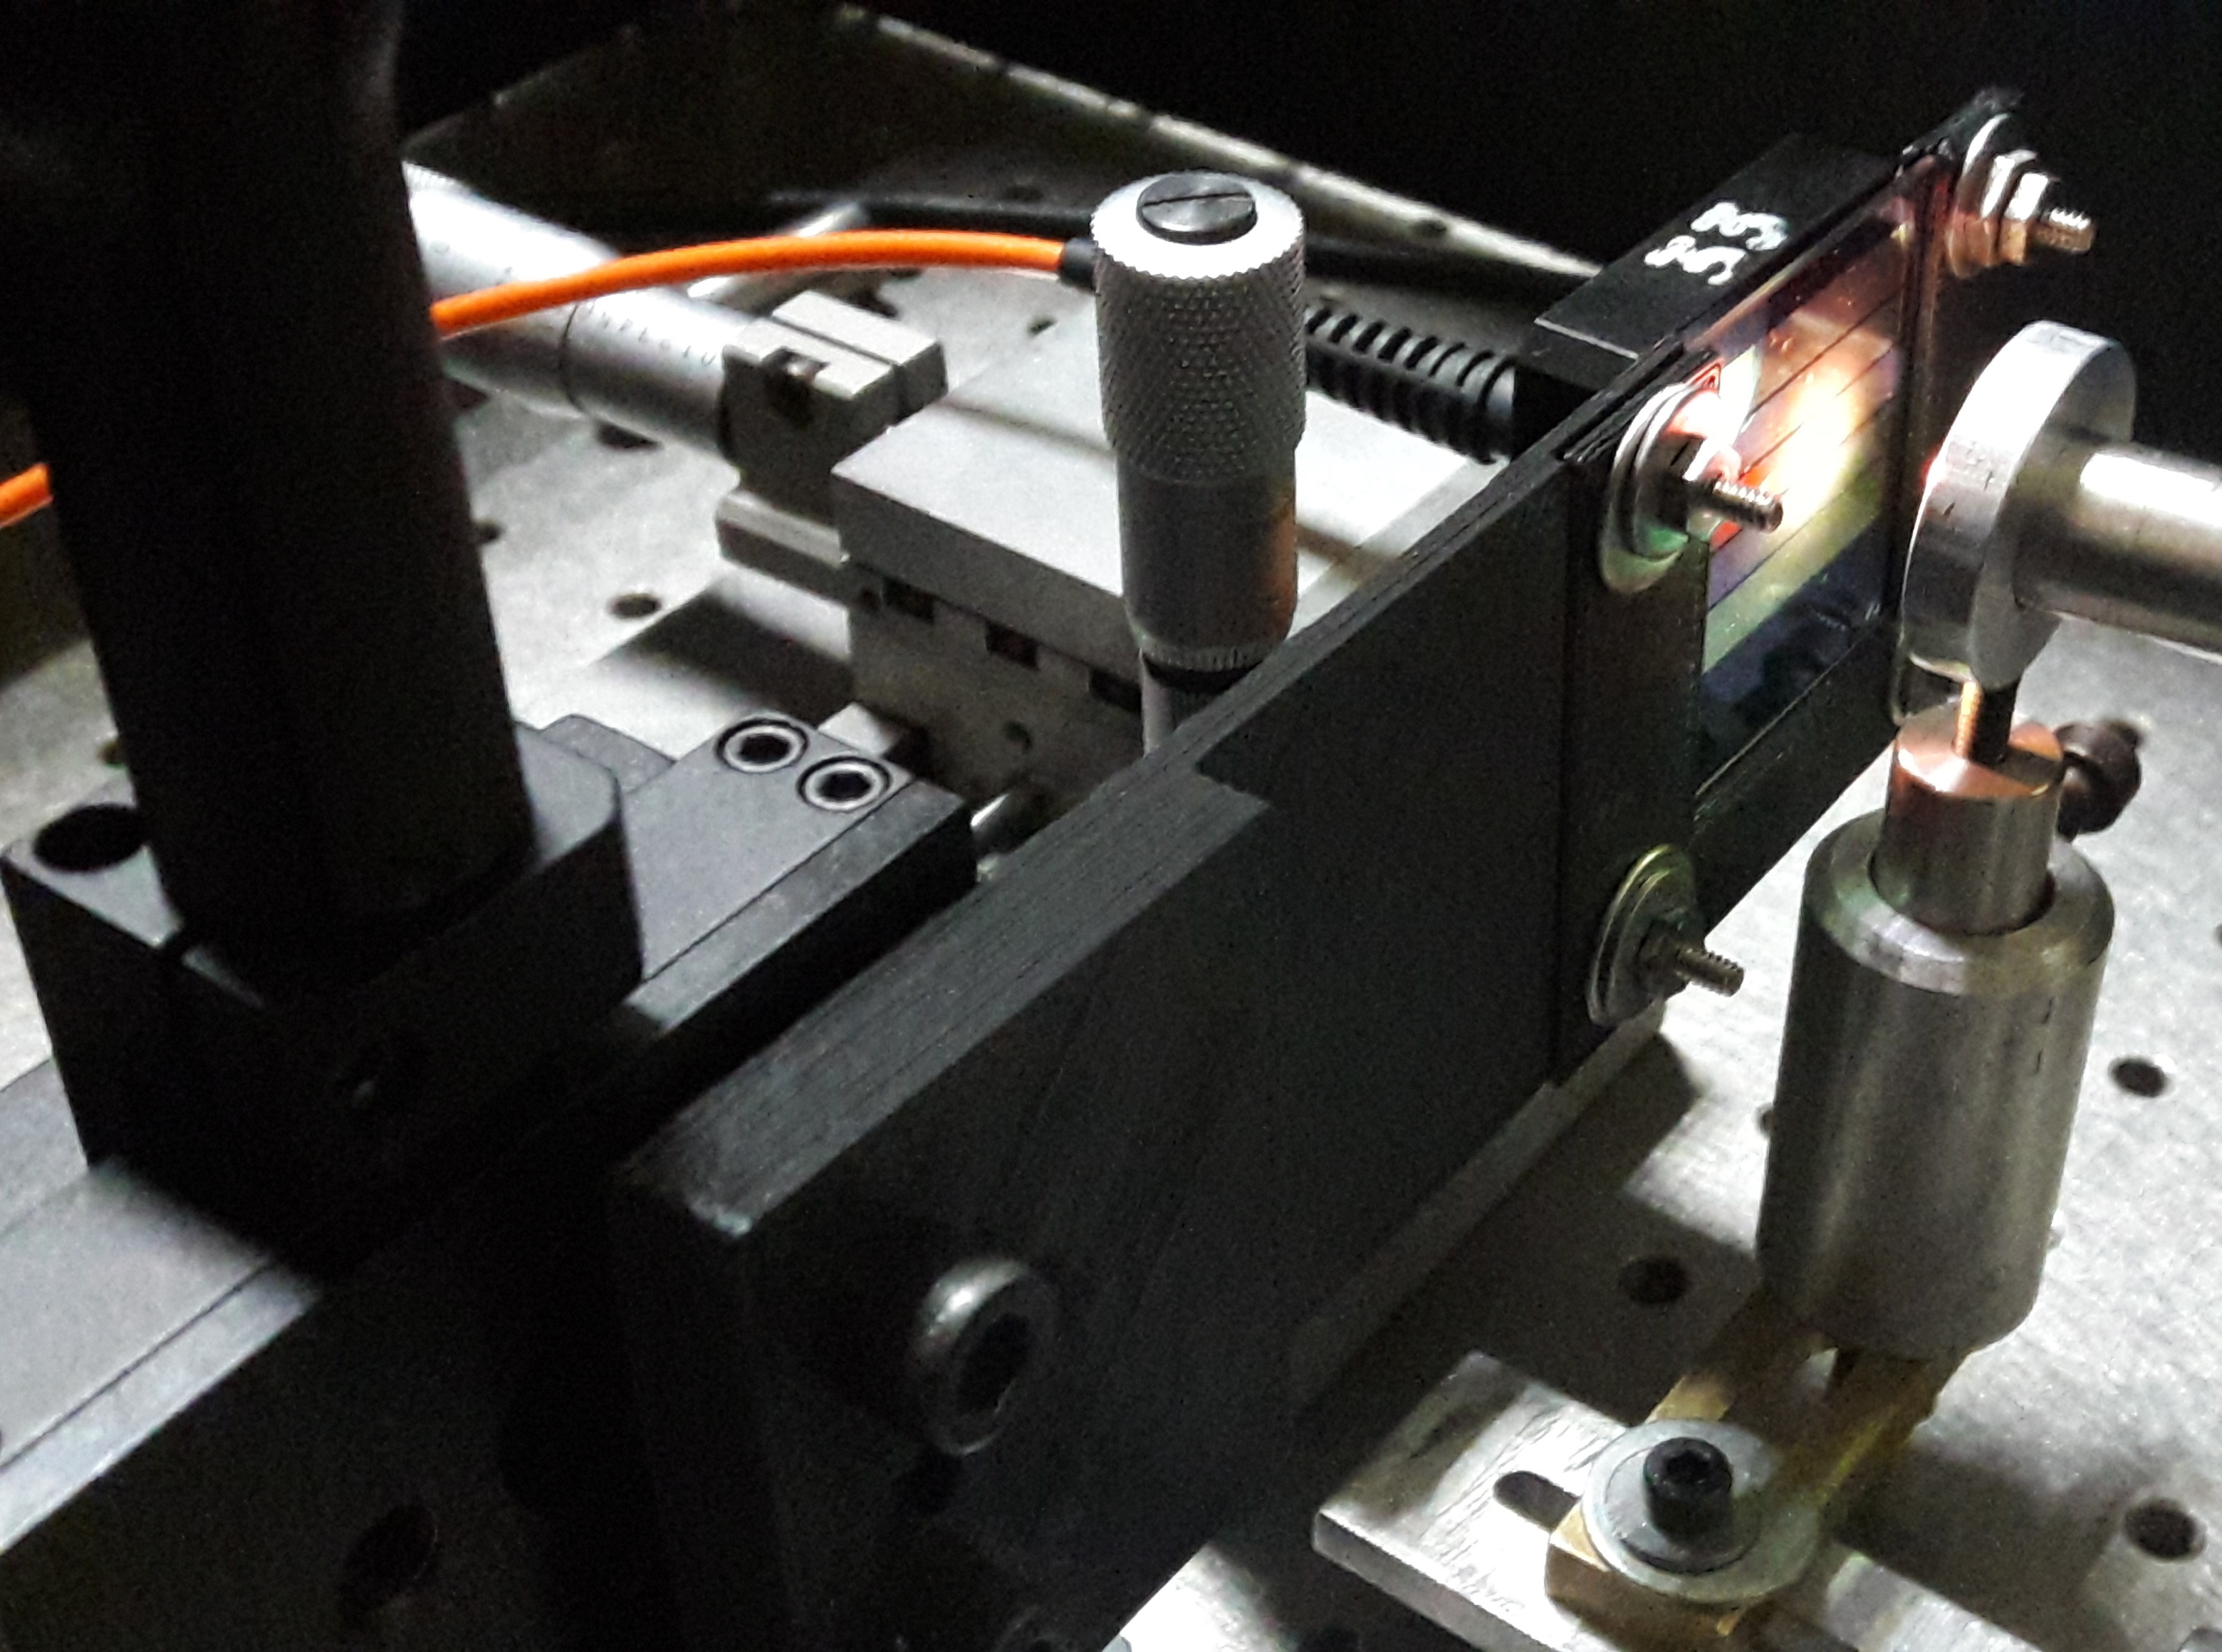
\includegraphics[scale=0.073]{Figs/microespectrometro/montajesetup0.jpg}
\hfill%
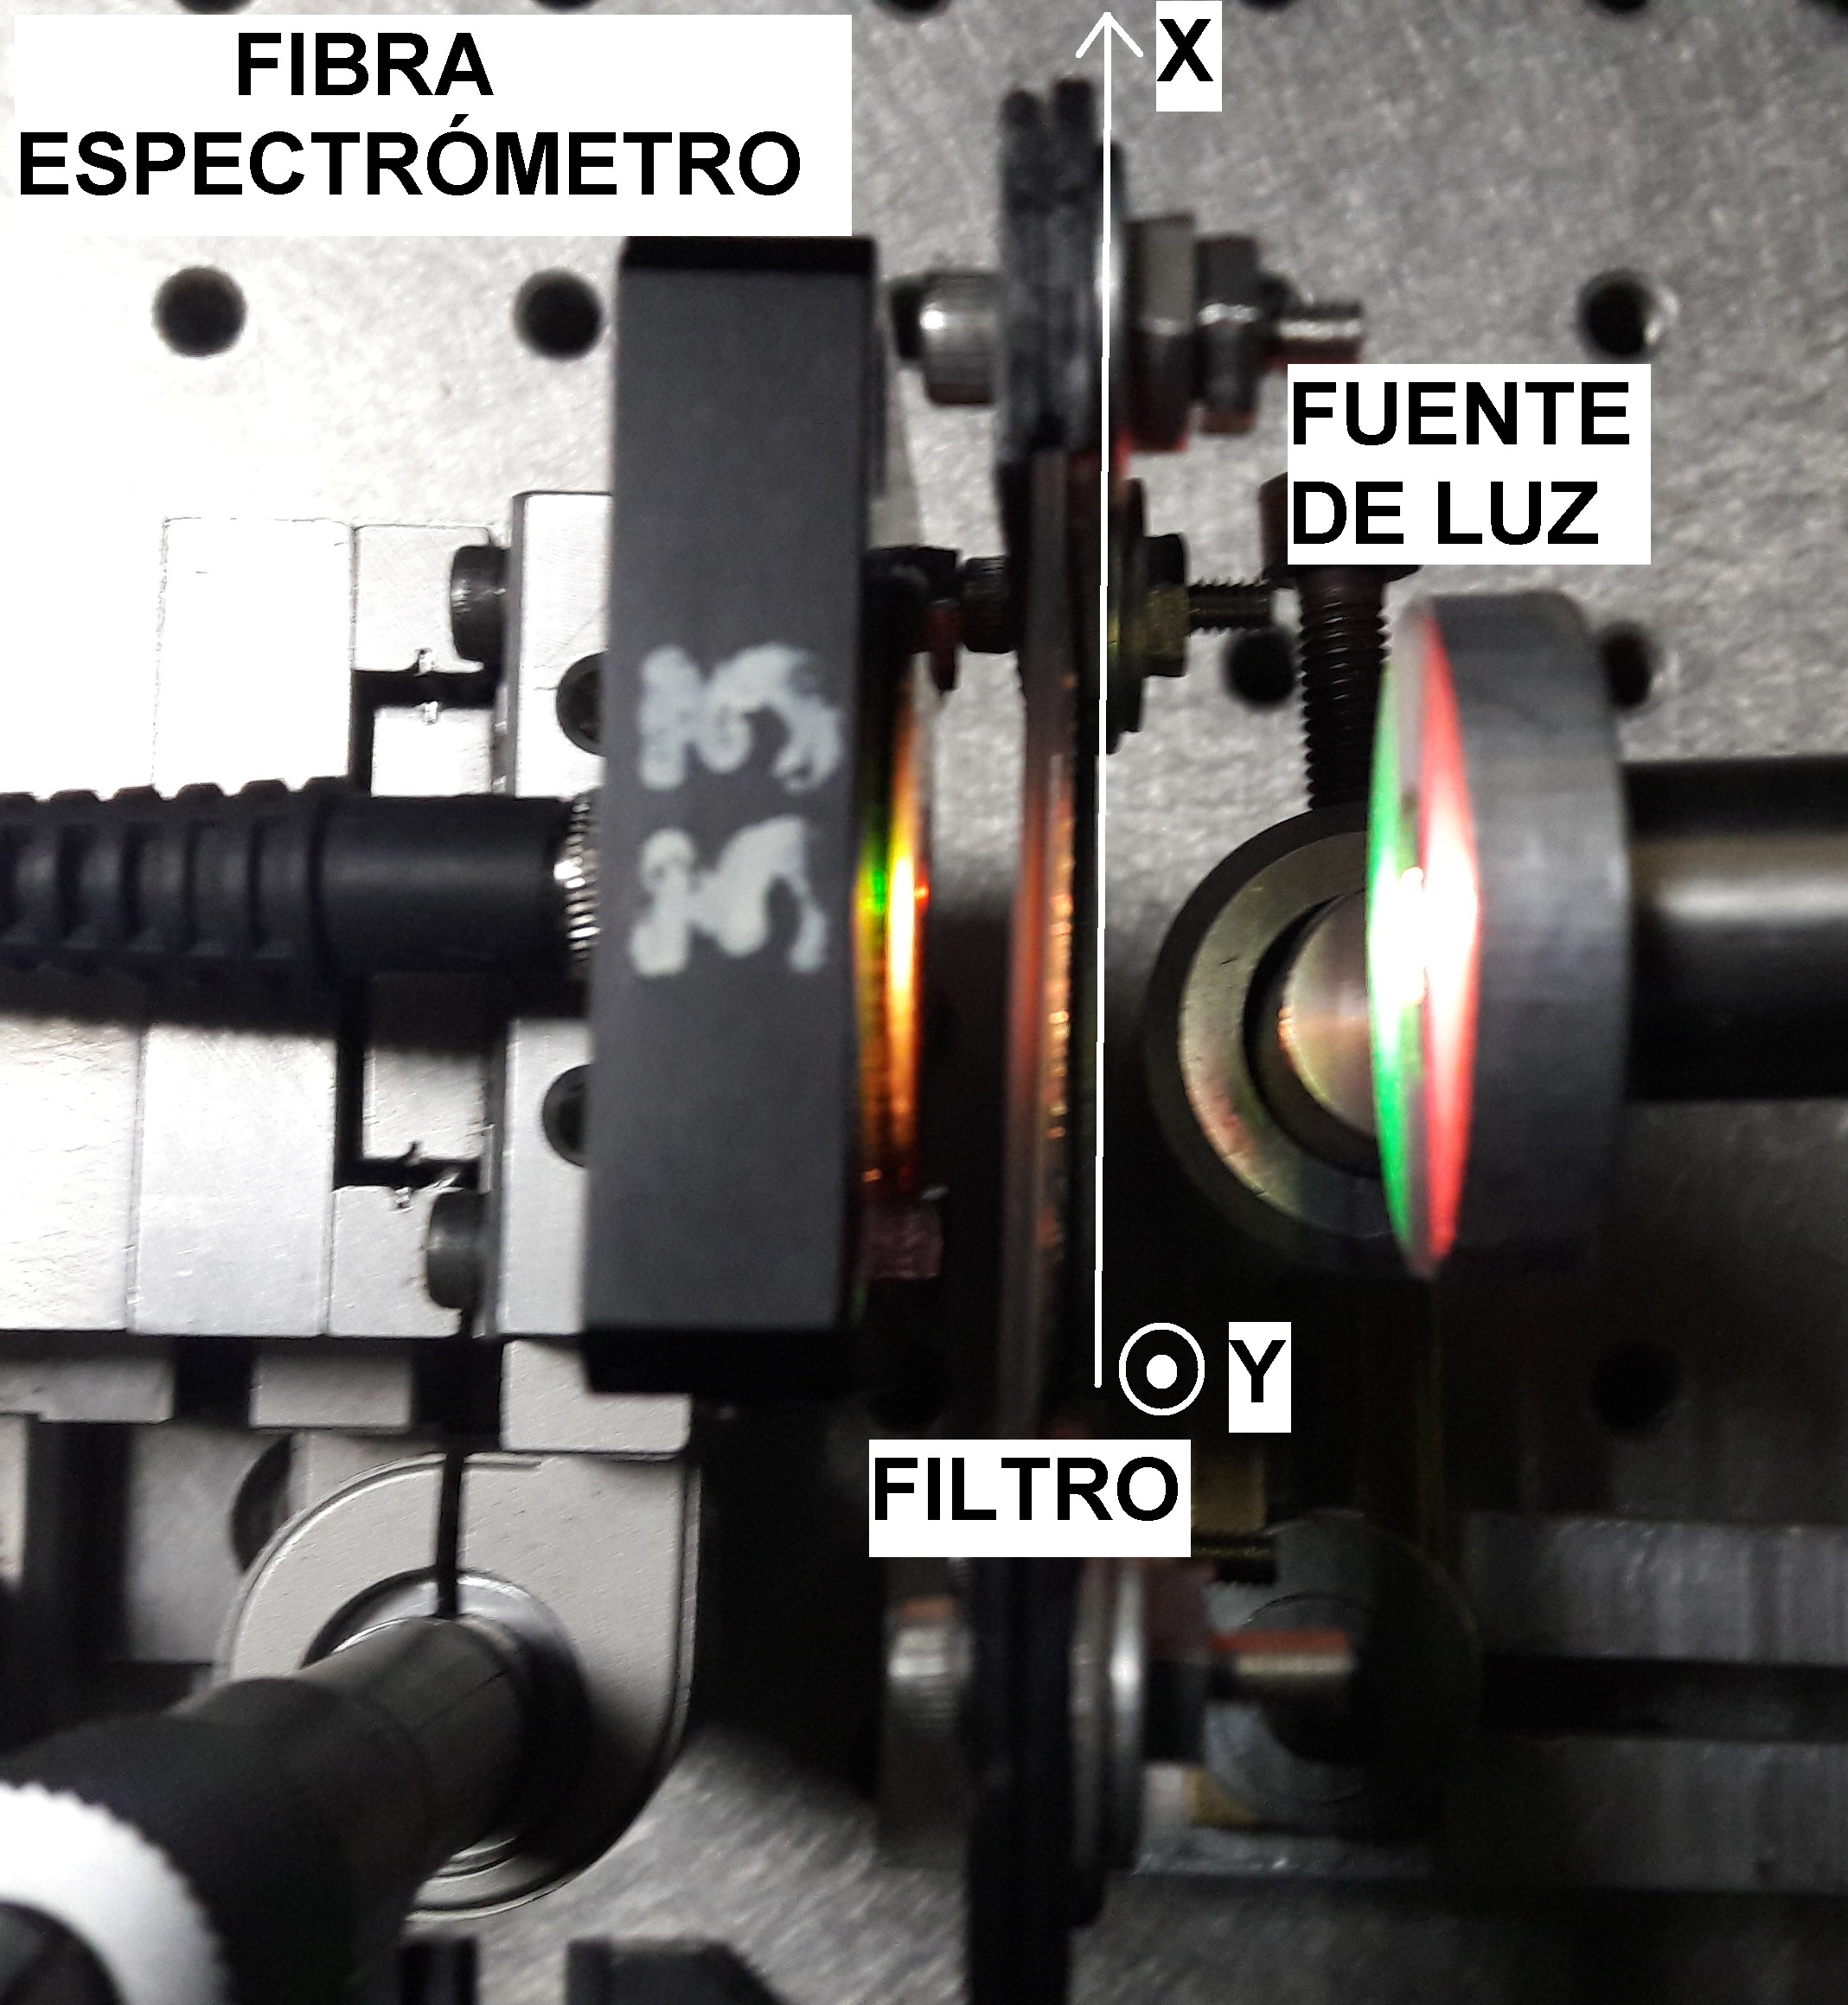
\includegraphics[scale=0.073]{Figs/microespectrometro/5.jpg}
\hfill%
\hfill%
\caption{(a) Arreglo experimental del prototipo preliminar. (b) Vista lateral del montaje del filtro sobre el soporte que se encuentra atornillado con unos tornillos M6 a la plataforma motorizada de Thorlabs. (c) El filtro se mueve en los ejes $\textit{x}$ e $\textit{y}$ definidos en la imagen, de forma perpendicular a la incidencia de la luz que define el eje z denominado óptico en adelante.}
\label{fig:p}
\end{figure}

Respecto del segundo objetivo específico propuesto relacionado con la determinación de un mapa multiespectral ($\textit{x}$,$\textit{y}$,$\lambda$) del filtro, se adquirió el espectro de transmisión de una región del filtro con dimensiones iguales 13 mm en el eje $\textit{x}$ y de 24.6 mm a lo largo del eje $\textit{y}$ (las cinco bandas junto al cromo que las separa tienen una altura de 25 mm (ver Figura \ref{fig:dimspost} (a)). El área del filtro adquirida fue el resultado de unir las mediciones de dos barridos cuyas dimensiones fueron para cada uno, de 13 mm a lo largo del eje $\textit{x}$ y de 12.3 mm a lo largo del eje $\textit{y}$. Los ejes fueron definidos de acuerdo al sistema de coordenadas de la Figura \ref{fig:p} (c) y el paso del desplazamiento de los motores de cada eje fue de 50 $\mu m$. La adquisición fue realizada en dos etapas debido a la limitación del recorrido de los tornillos desplazados por los motores paso a paso como se explicó anteriormente. De esta manera se adquirió en primer lugar la región superior del filtro que contiene a las bandas azul, verde y parte de la pancromática con una cierta altura de la fuente de luz y de la fibra del espectrómetro. La fuente y la fibra se encontraban montadas sobre unos posicionadores micrométricos con los cuales se varió su altura respecto del filtro para poder medir la región inferior del filtro que contenía la región no medida de la banda pancromática, la banda roja y la banda del NIR. La fuente de luz y la fibra del espectrómetro fueron posicionadas lo más cerca posible del filtro, sin intervenir su libre desplazamiento para realizar el barrido, con el fin de minimizar el tiempo de integración de cada medición del espectro de transmisión que fue de 1 ms.

Con el objetivo de visualizar una imagen completa del filtro como la que se obtuvo con el microscopio Zeiss (Ver Figura \ref{fig:supsfiltro}) pero que contenga además la información espectral de cada medición se desarrolló una interfaz gráfica interactiva que se muestra en la Figura \ref{fig:GUI00}.

\begin{figure}[H]
	\centering
	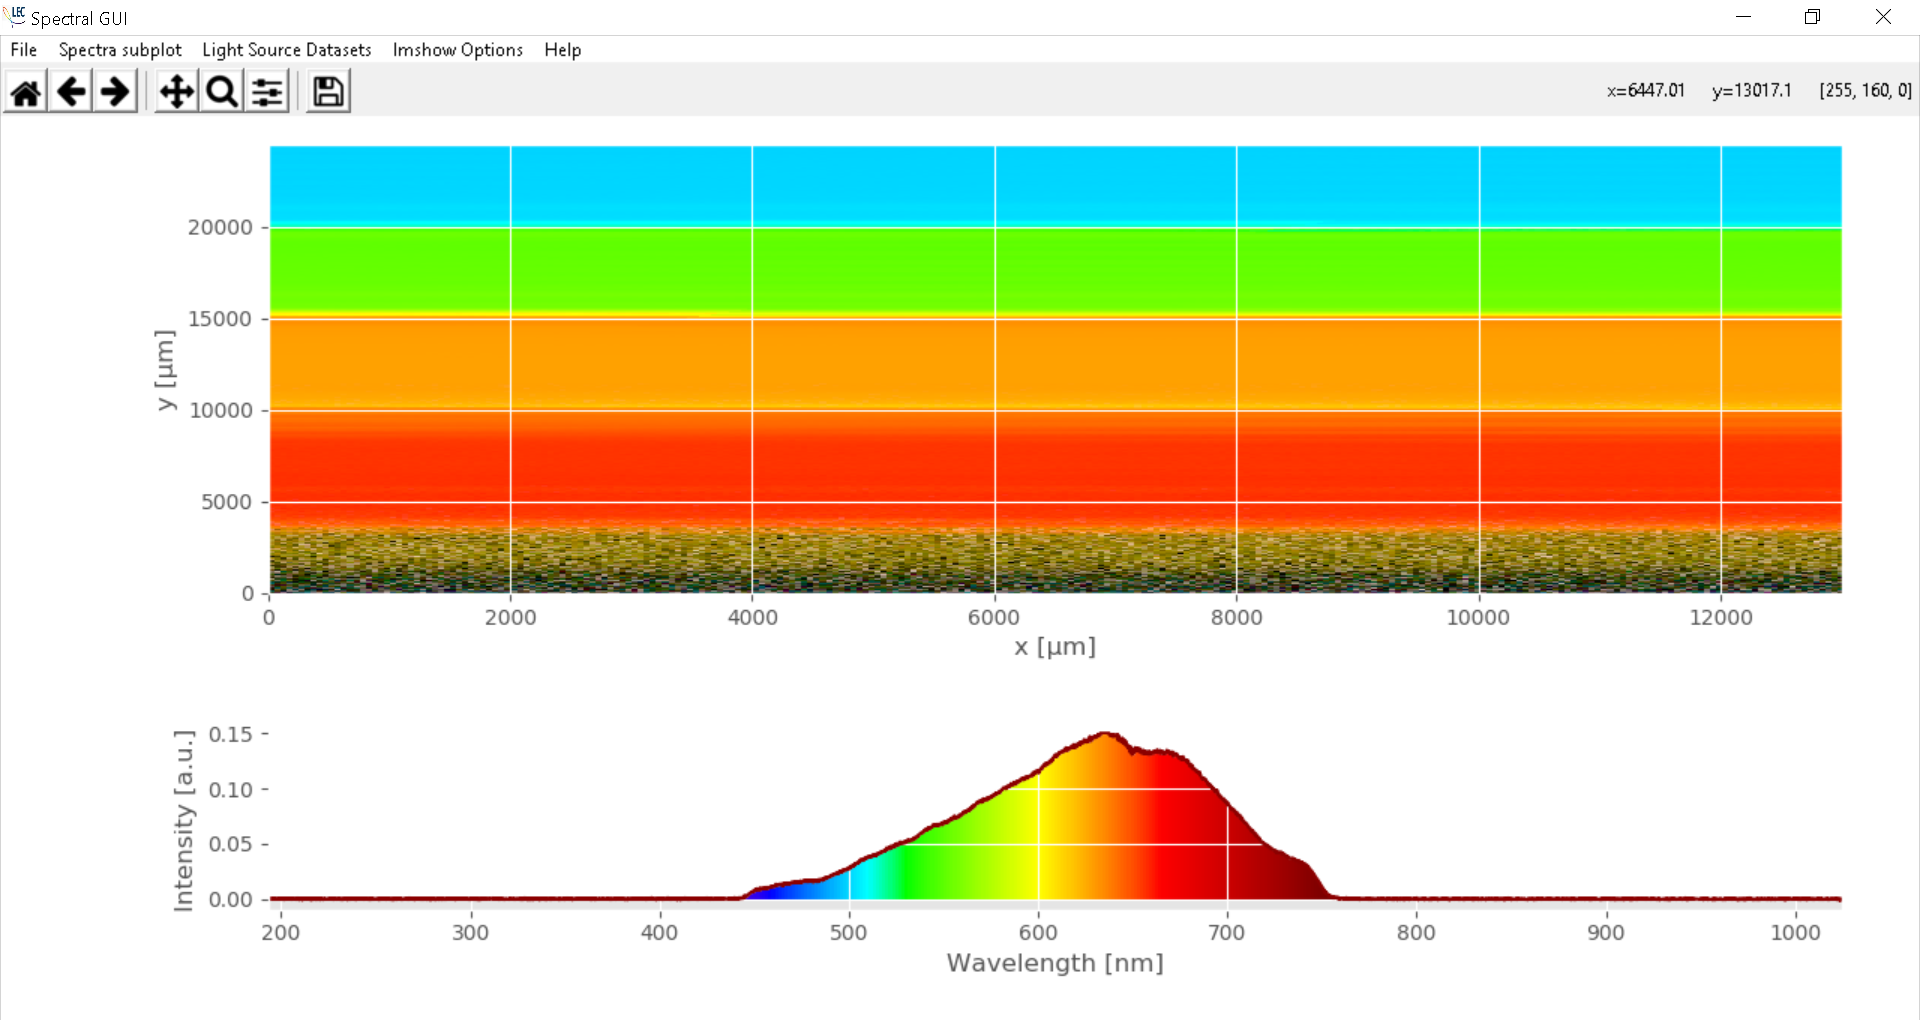
\includegraphics[width=1.0\textwidth]{Figs/microespectrometro/guirgb.png}
	\caption{Interfaz gráfica cuyo \textit{imshow} tenía una paleta de colores del espectro visible, de acuerdo al espacio de color CIE XYZ \cite{Wyman}.}
	\label{fig:GUI00}
\end{figure}


La interfaz gráfica fue realizada [\href{https://github.com/jrr1984/Prototipo0\_S-D\_SpectralGUI/blob/master/spectral\_gui/main.py}{\faGithub$_{3.1.2}$}] con la librería \href{https://wiki.python.org/moin/TkInter}{\textit{Tkinter}}. El barrido completo que se muestra en la imagen del mapa de colores de la Figura \ref{fig:GUI00} estuvo compuesto por 127920 mediciones de espectros de transmisión, que tomaron aproximadamente 18 horas de medición en total. Con la librería \href{https://pypi.org/project/colorpy/}{ColorPy} se obtuvo una tupla RGB a partir del espectro medido y cada tupla fue asignada a la posición medida del filtro. El conjunto total de todas las posiciones del filtro medidas estuvo formado por una matriz de 492 filas y 260 columnas. Dicha matriz fue mostrada como una imagen RGB con el método \textit{imshow} de la librería \textit{Matplotlib}. El gráfico debajo del \textit{imshow} muestra el espectro medido (gráfico de la intensidad detectada en función de la longitud de onda) para el píxel de la imagen sobre el cual se posicione el \textit{mouse} de forma actualizada y no muestra nada si se posiciona el mouse fuera de la imagen. 

En lugar de la imagen RGB de las mediciones también se puede mostrar el $\chi^{2}$ del espectro de transmisión de cada banda lo que permitiría ver la homogeneidad del espectro de transmisión de cada banda, que fue definido para la medición asociada a una posición (i,j) de cada banda de la siguiente manera:
\begin{equation}
\chi^{2}_{banda}(i,j) = \sum \frac{(medici\acute{o}n_{i,j} - espectro\_medio_{banda})^{2}}{medici\acute{o}n^{2}_{i,j}}
\end{equation}
donde $espectro\_medio_{banda}$ es el resultado de tomar el valor medio de todas las mediciones de una banda. En la Figura \ref{fig:GUI01} se muestra una región del filtro que contiene al cromo (en falso color amarillo) que separa la banda pancromática de la banda verde. 

La interfaz gráfica permite además graficar el espectro de un cierto píxel de la imagen generada a partir de la selección con el mouse, guardar imágenes de la región de interés, mostrar el espectro de la fuente de luz utilizada, etc, todas opciones que se consideraron útiles para la caracterización de las propiedades ópticas del filtro y deseadas para el prototipo final del equipo.

\begin{figure}[H]
	\centering
	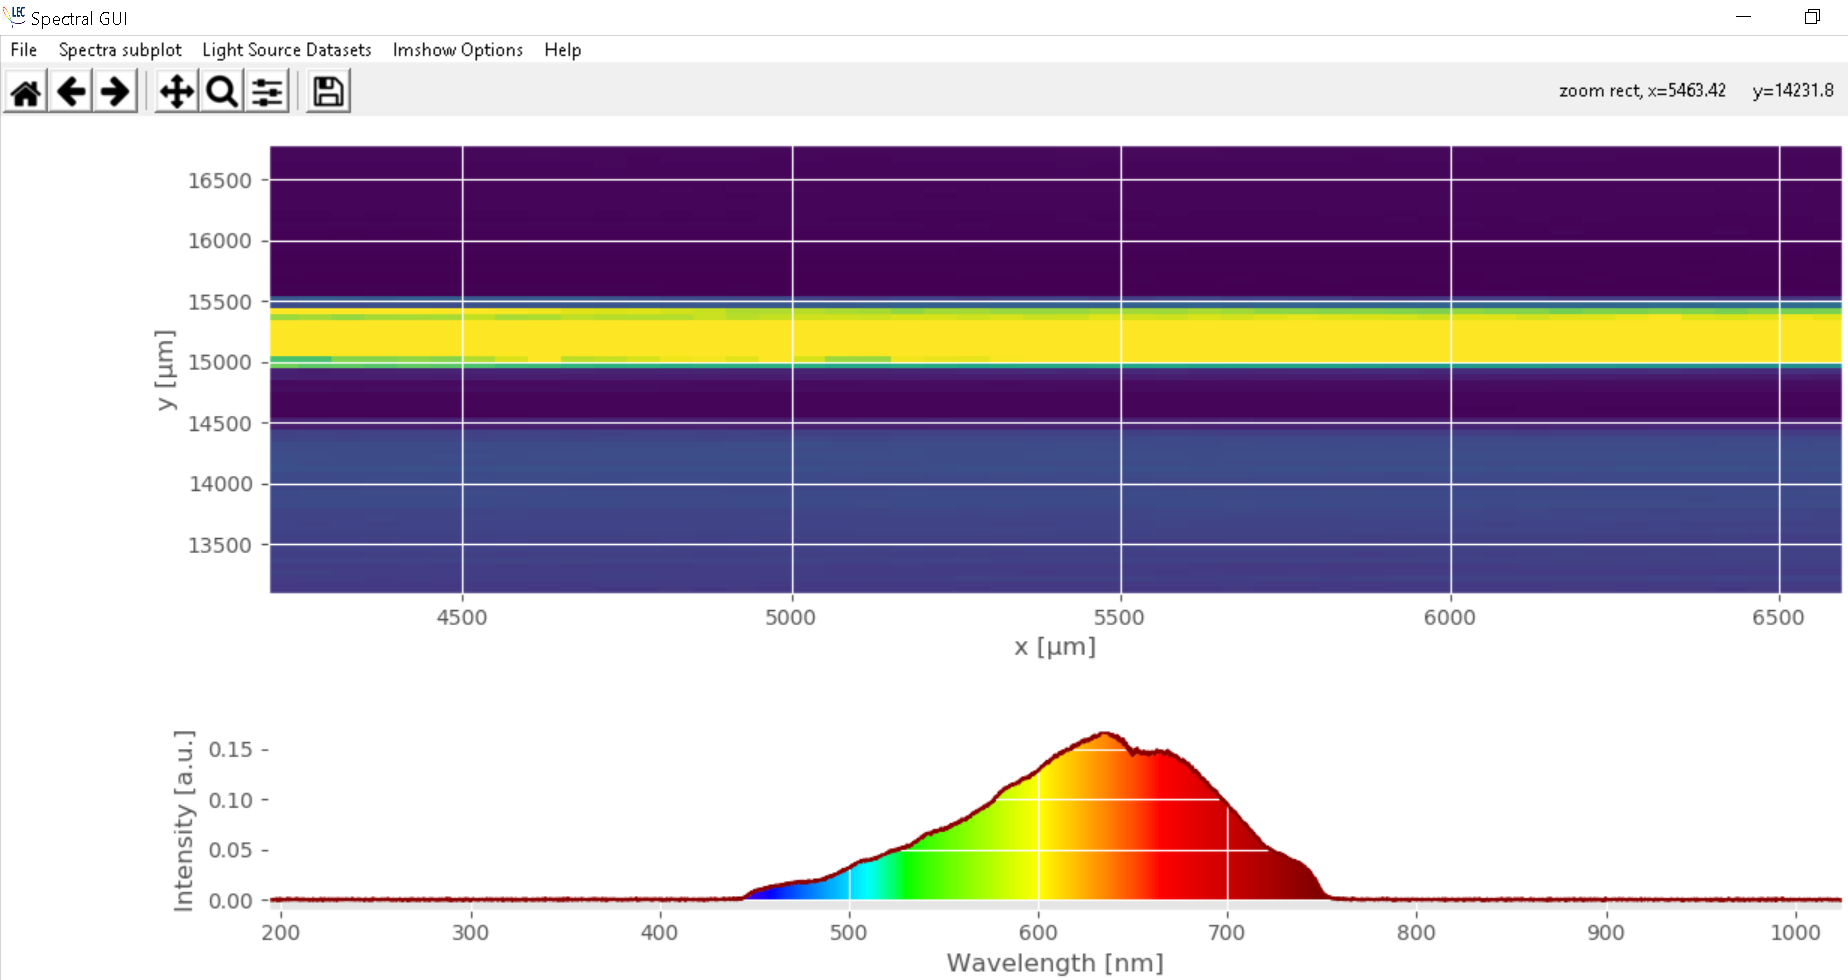
\includegraphics[width=1.0\textwidth]{Figs/microespectrometro/chidisp.png}
	\caption{Interfaz gráfica con el \textit{imshow} del $\chi^{2}$ de cada banda. \textit{Zoom} sobre el cromo que separa la banda pancromática de la banda verde.}
	\label{fig:GUI01}
\end{figure}

El prototipo preliminar permitió establecer las características deseadas del equipo final y evaluar su factibilidad sin incurrir en gastos importantes de prototipado. A este prototipo se le propusieron las siguientes mejoras que fueron incluidas en el montaje y construcción del microespectrómetro [\ref{sec:montcontmsp}]:

\begin{enumerate}
\justifying
\item \texttt{Fuente de luz [\ref{sec:fteluzyesp}]}: Se modificó la fuente de luz de \textit{Fiber-Lite} que consiste de un \textit{fiber bundle} (arreglo de fibras ópticas) de un diámetro de 4.8 mm por una fuente de luz acoplada con una fibra óptica multimodo cuya apertura numérica fue de 0.22 y cuyo \textit{core} tenía un diámetro de 200 $\mu m$. Se decidió optar por la fuente de luz cuya salida divergente tuviera el menor ángulo del cono de luz de salida. Este criterio de diseño tenía como objetivo disminuir la región iluminada del filtro por la fuente de luz, lo que reduciría ciertas reflexiones espurias en los componentes ópticos del microespectrómetro provenientes de la luz de regiones no alcanzadas por el área de adquisición del microespectrómetro. Este efecto que aumenta proporcionalmente a la relación entre el área iluminada y el área adquirida del filtro se denomina efecto de Schwarzchild-Villiger \cite{Naora279} y debería ser considerado en las futuras mejoras del equipo aquí propuesto. Además la nueva fuente de luz utilizada tenía la misma fibra óptica que el espectrómetro, hecho que permitió realizar fácilmente la identificación de la región medida con el espectrómetro respecto de la imagen adquirida con la cámara (Ver Sección \ref{sec:camwebgui}).
\item \texttt{Rango de barrido [\ref{sec:platina}]}: Como la plataforma motorizada de Thorlabs utilizada en el prototipo preliminar tenía un límite de recorrido de 13 mm x 13 mm, no se podía adquirir el espectro de transmisión del filtro completo cuya región que contiene a las cinco bandas tiene unas dimensiones de 27 mm x 25 mm. En consecuencia se desarrolló una platina motorizada con el suficiente recorrido para poder realizar el barrido completo del filtro y también se consideró el paso y precisión mecánicas mínimas como para poder adquirir áreas de defectos de diámetro mayor a 20 $\mu m$ con la mayor cantidad de puntos posible, de forma tal de poder aprovechar el poder de resolución del microespectrómetro.
\item \texttt{Microespectrómetro [\ref{sec:montalin}]}: Se montó un microespectrómetro con una resolución óptica lateral diseñado para caracterizar defectos de diámetro mayor a 20 $\mu m$.
\item \texttt{Integración de una cámara [\ref{sec:camwebgui}]}: Se incorporó una cámara y un  \textit{joystick} al equipo para poder seleccionar la región del filtro a medir y se desarrolló una interfaz gráfica para poder visualizar en simultáneo la imagen digital de dicha región y el espectro de transmisión. 
\end{enumerate}
	
%%%%%%%%%%%%%%%%%%%%%%%%%%%%%%%%%%%%%%%%%%%%%%%%%%%%%%%%%%%%%%%%%%%%%%%%%%%%%%%%%%%%%%%%%%%%%%%%%%%%%%%%%%%%%%%%%%%%%%%%%%%%%%%%%%%%%%%%%%%%%%%%%%%%%%%%%%%%%%%%%%%%%%%%%%%%%%%%%%%%%%%%%%%%%%%%%%%%%%%%%%%%%%%%%%%%%%%%%%%%
\singlespacing
\section{Diseño y construcción del microespectrómetro}
\label{sec:montcontmsp}
\spacing{1.5}

\hspace{0.5cm}En esta sección se describen los criterios de diseño y todas las consideraciones técnicas del microespectrómetro, de la platina motorizada desarrollada que fue controlada con un \textit{joystick} y de la cámara integrada. En la Figura \ref{fig:presequipo} se muestra la última versión del equipo desarrollado. En las siguientes secciones se describen cada una de las partes del instrumento. El equipo final desarrollado de forma modular puede ser adaptado a requerimientos ópticos y mecánicos específicos distintos a los presentados en esta tesis. 
\begin{figure}[H]
	\centering
	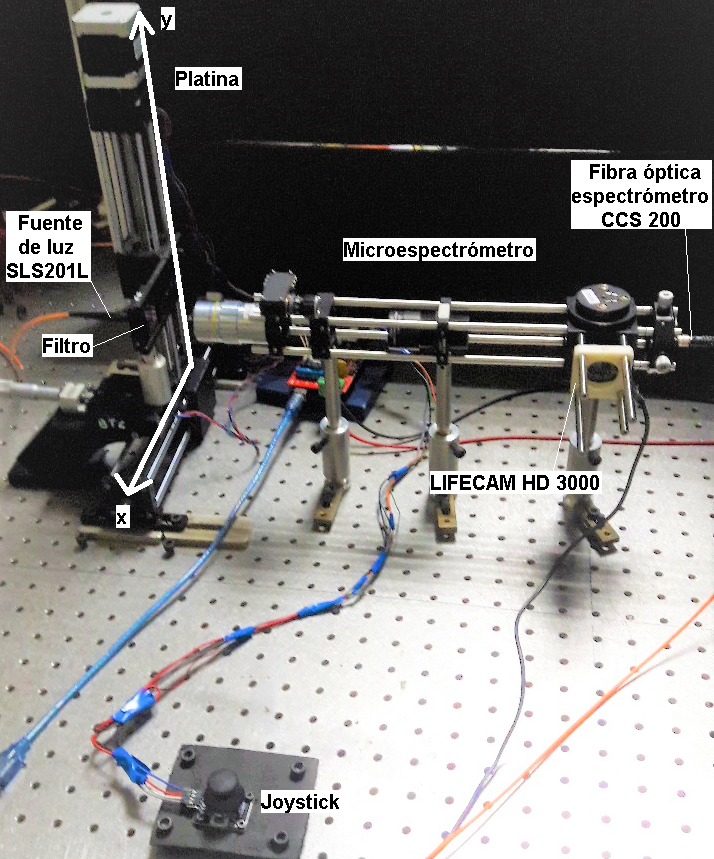
\includegraphics[width=1.0\textwidth]{Figs/microespectrometro/presentacion_equipo.png}
	\caption{Imagen de la última versión del equipo desarrollado.}
	\label{fig:presequipo}
\end{figure}




%%%%%%%%%%%%%%%%%%%%%%%%%%%%%%%%%%%%%%%%%%%%%%%%%%%%%%%%%%%%%%%%%%%%%%%%%%%%%%%%%%%%%%%%%%%%%%%%%%%%%%%%%%%%%%%%%%%%%%%%%%%%%%%%%%%%%%%%%%%%%%%%%%%%%%%%%%%%%%%%%%%%%%%%%%%%%%%%%%%%%%%%%%%%%%%%%%%%%%%%%%%%%%%%%%%%%%%%%%%%

\singlespacing
\subsection{Fuente de luz y espectrómetro \href{https://github.com/jrr1984/defects_analysis/blob/master/light_sources_spectrum.py}{\faGithub$_{3.2.1}$}}
\label{sec:fteluzyesp}
\spacing{1.5}

\hspace{0.5cm}El criterio de elección de la fuente de luz dependió fundamentalmente del rango de longitudes de onda que se quiso medir, que para el caso del filtro aquí analizado dicho rango se encontró entre los 450 nm y los 900 nm.
Se utilizó una fuente de luz halógena y de tungsteno modelo \href{https://www.thorlabs.com/newgrouppage9.cfm?objectgroup_id=7269&pn=SLS201L/M}{SLS201L} del fabricante Thorlabs (Ver Figura \ref{fig:fuentesp} (a)). 

\begin{figure}[H]
%\centering
\hfill%
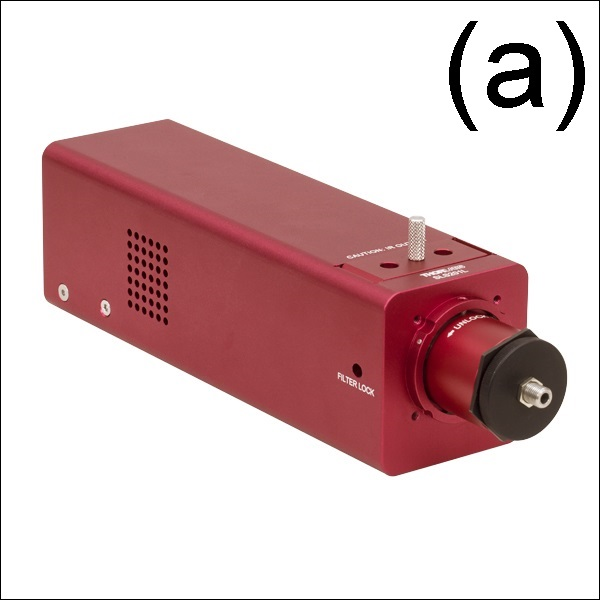
\includegraphics[scale=0.5]{Figs/microespectrometro/sls201l.jpg}
\hfill%
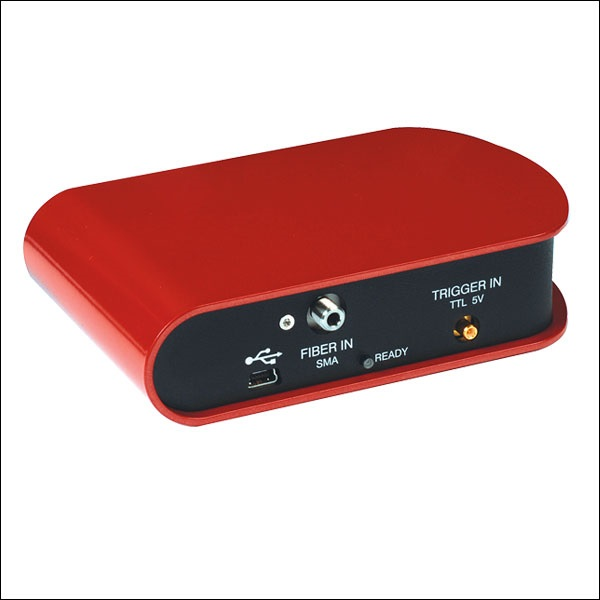
\includegraphics[scale=0.5]{Figs/microespectrometro/ccs200.jpg}
\hfill%
\hfill%
\caption{(a) Imagen de la fuente de luz \href{https://www.thorlabs.com/newgrouppage9.cfm?objectgroup\_id=7269\&pn=SLS201L/M}{SLS201L} del fabricante Thorlabs. (b) Imagen del espectrómetro \href{https://www.thorlabs.com/thorproduct.cfm?partnumber=CCS200/M\#ad-image-0}{CCS200/M} del fabricante Thorlabs.}
\label{fig:fuentesp}		
\end{figure}

En la Figura \ref{fig:espfth} se muestra el espectro de emisión de la fuente de luz utilizada.  El espectrómetro utilizado para realizar las mediciones fue el \href{https://www.thorlabs.com/thorproduct.cfm?partnumber=CCS200/M#ad-image-0}{CCS200/M} del fabricante Thorlabs (Ver Figura \ref{fig:fuentesp} (b)).El espectro de emisión de la fuente de luz reportado por el fabricante indica que debería ser en el rango de longitudes de onda de 360 - 2600 nm, lo cual se pudo verificar por lo menos en el rango comprendido entre los 200 nm y los 1000 nm que es el rango de detección del espectrómetro. El fabricante reportó una precisión del espectrómetro menor a los 2 nm y el tiempo de integración del detector de entre 10 $\mu s$ y 60 s. La fuente de luz \href{https://www.thorlabs.com/newgrouppage9.cfm?objectgroup_id=7269&pn=SLS201L/M}{SLS201L} (Ver Figura \ref{fig:fuentesp} (a)) del fabricante Thorlabs tiene una salida acoplada con una fibra óptica multimodo \href{https://www.thorlabs.com/newgrouppage9.cfm?objectgroup_id=6839&pn=FG200UCC}{FG200UCC} de una apertura numérica igual a 0.22 y cuyo \textit{core} tiene un diámetro de 200 $\mu m$. La fibra óptica de la fuente de luz es idéntica a la fibra óptica del espectrómetro. El conector SMA de la fibra óptica de color naranja que se muestra en la Figura \ref{fig:montttluz} fue conectado al adaptador \href{https://www.thorlabs.com/thorproduct.cfm?partnumber=SM1SMA\#ad-image-0}{SM1SMA} y éste a su vez fue montado sobre un \textit{cage} \href{https://www.thorlabs.com/thorproduct.cfm?partnumber=CP33}{CP33}. Al mismo tiempo dicho \textit{cage} fue montado con un vástago y una torreta a un posicionador micrométrico que permitió disminuir la distancia entre la fuente de luz y el filtro, de manera tal de poder reducir los tiempos de integración de la luz y en consecuencia reducir los tiempos de duración de cada barrido de una cierta región del filtro.

\begin{figure}[H]
	\centering
	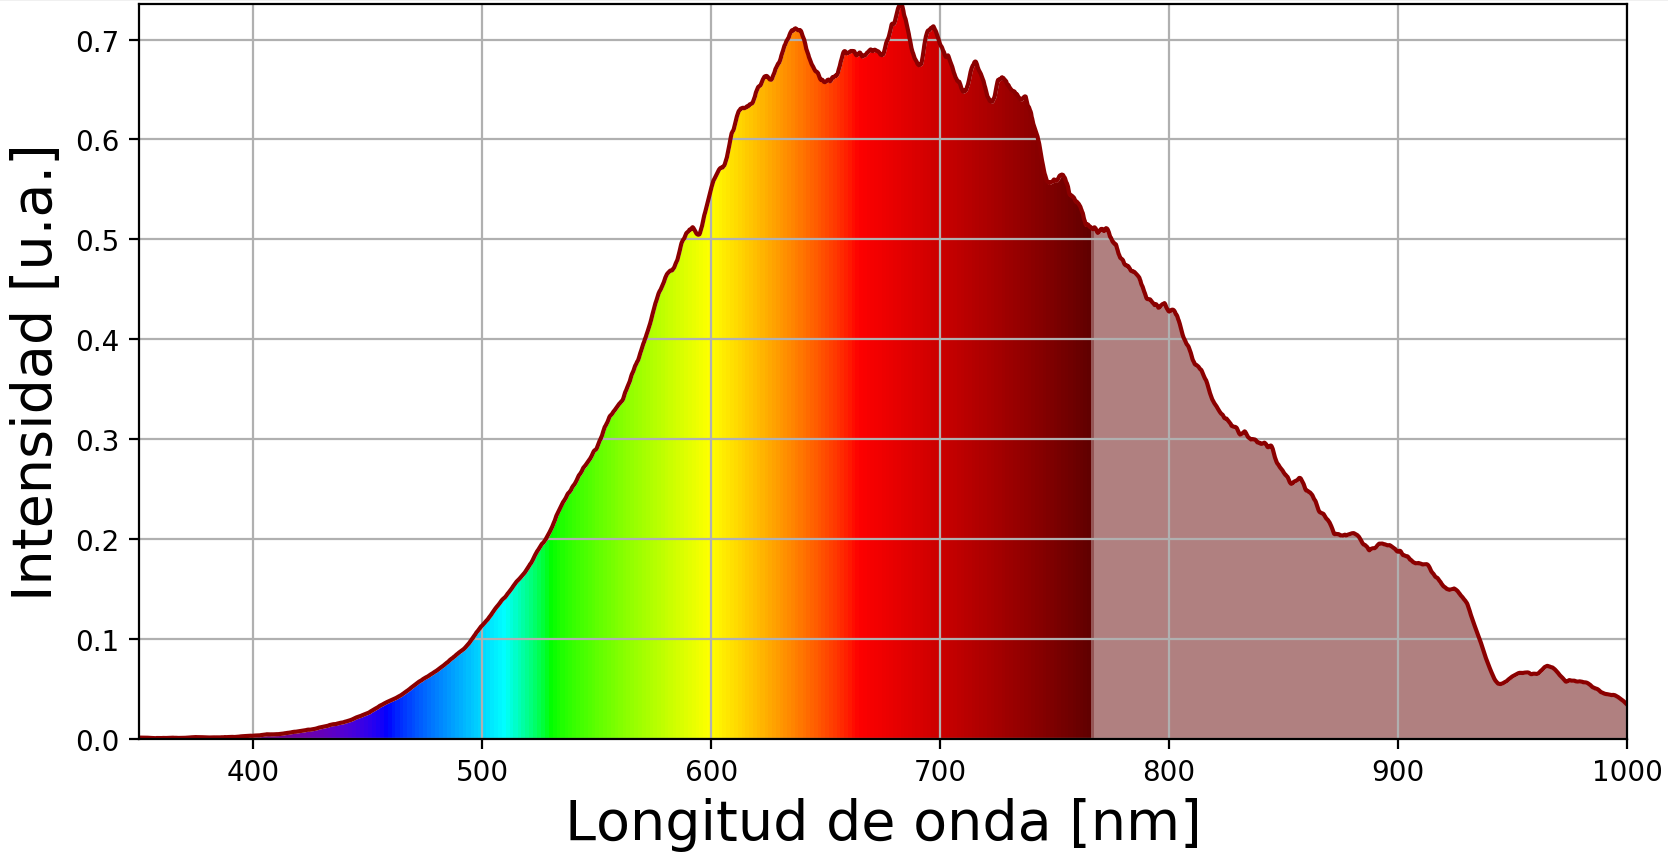
\includegraphics[scale=0.45]{Figs/microespectrometro/espfuentethorl.png}
	\caption{Espectro de emisión de la fuente de luz \href{https://www.thorlabs.com/newgrouppage9.cfm?objectgroup\_id=7269&pn=SLS201L/M}{SLS201L} del fabricante Thorlabs [\href{https://github.com/jrr1984/defects\_analysis/blob/master/light\_sources\_spectrum.py}{\faGithub$_{3.2.1}$}].}
	\label{fig:espfth}
\end{figure}

\begin{figure}[H]
	\centering
	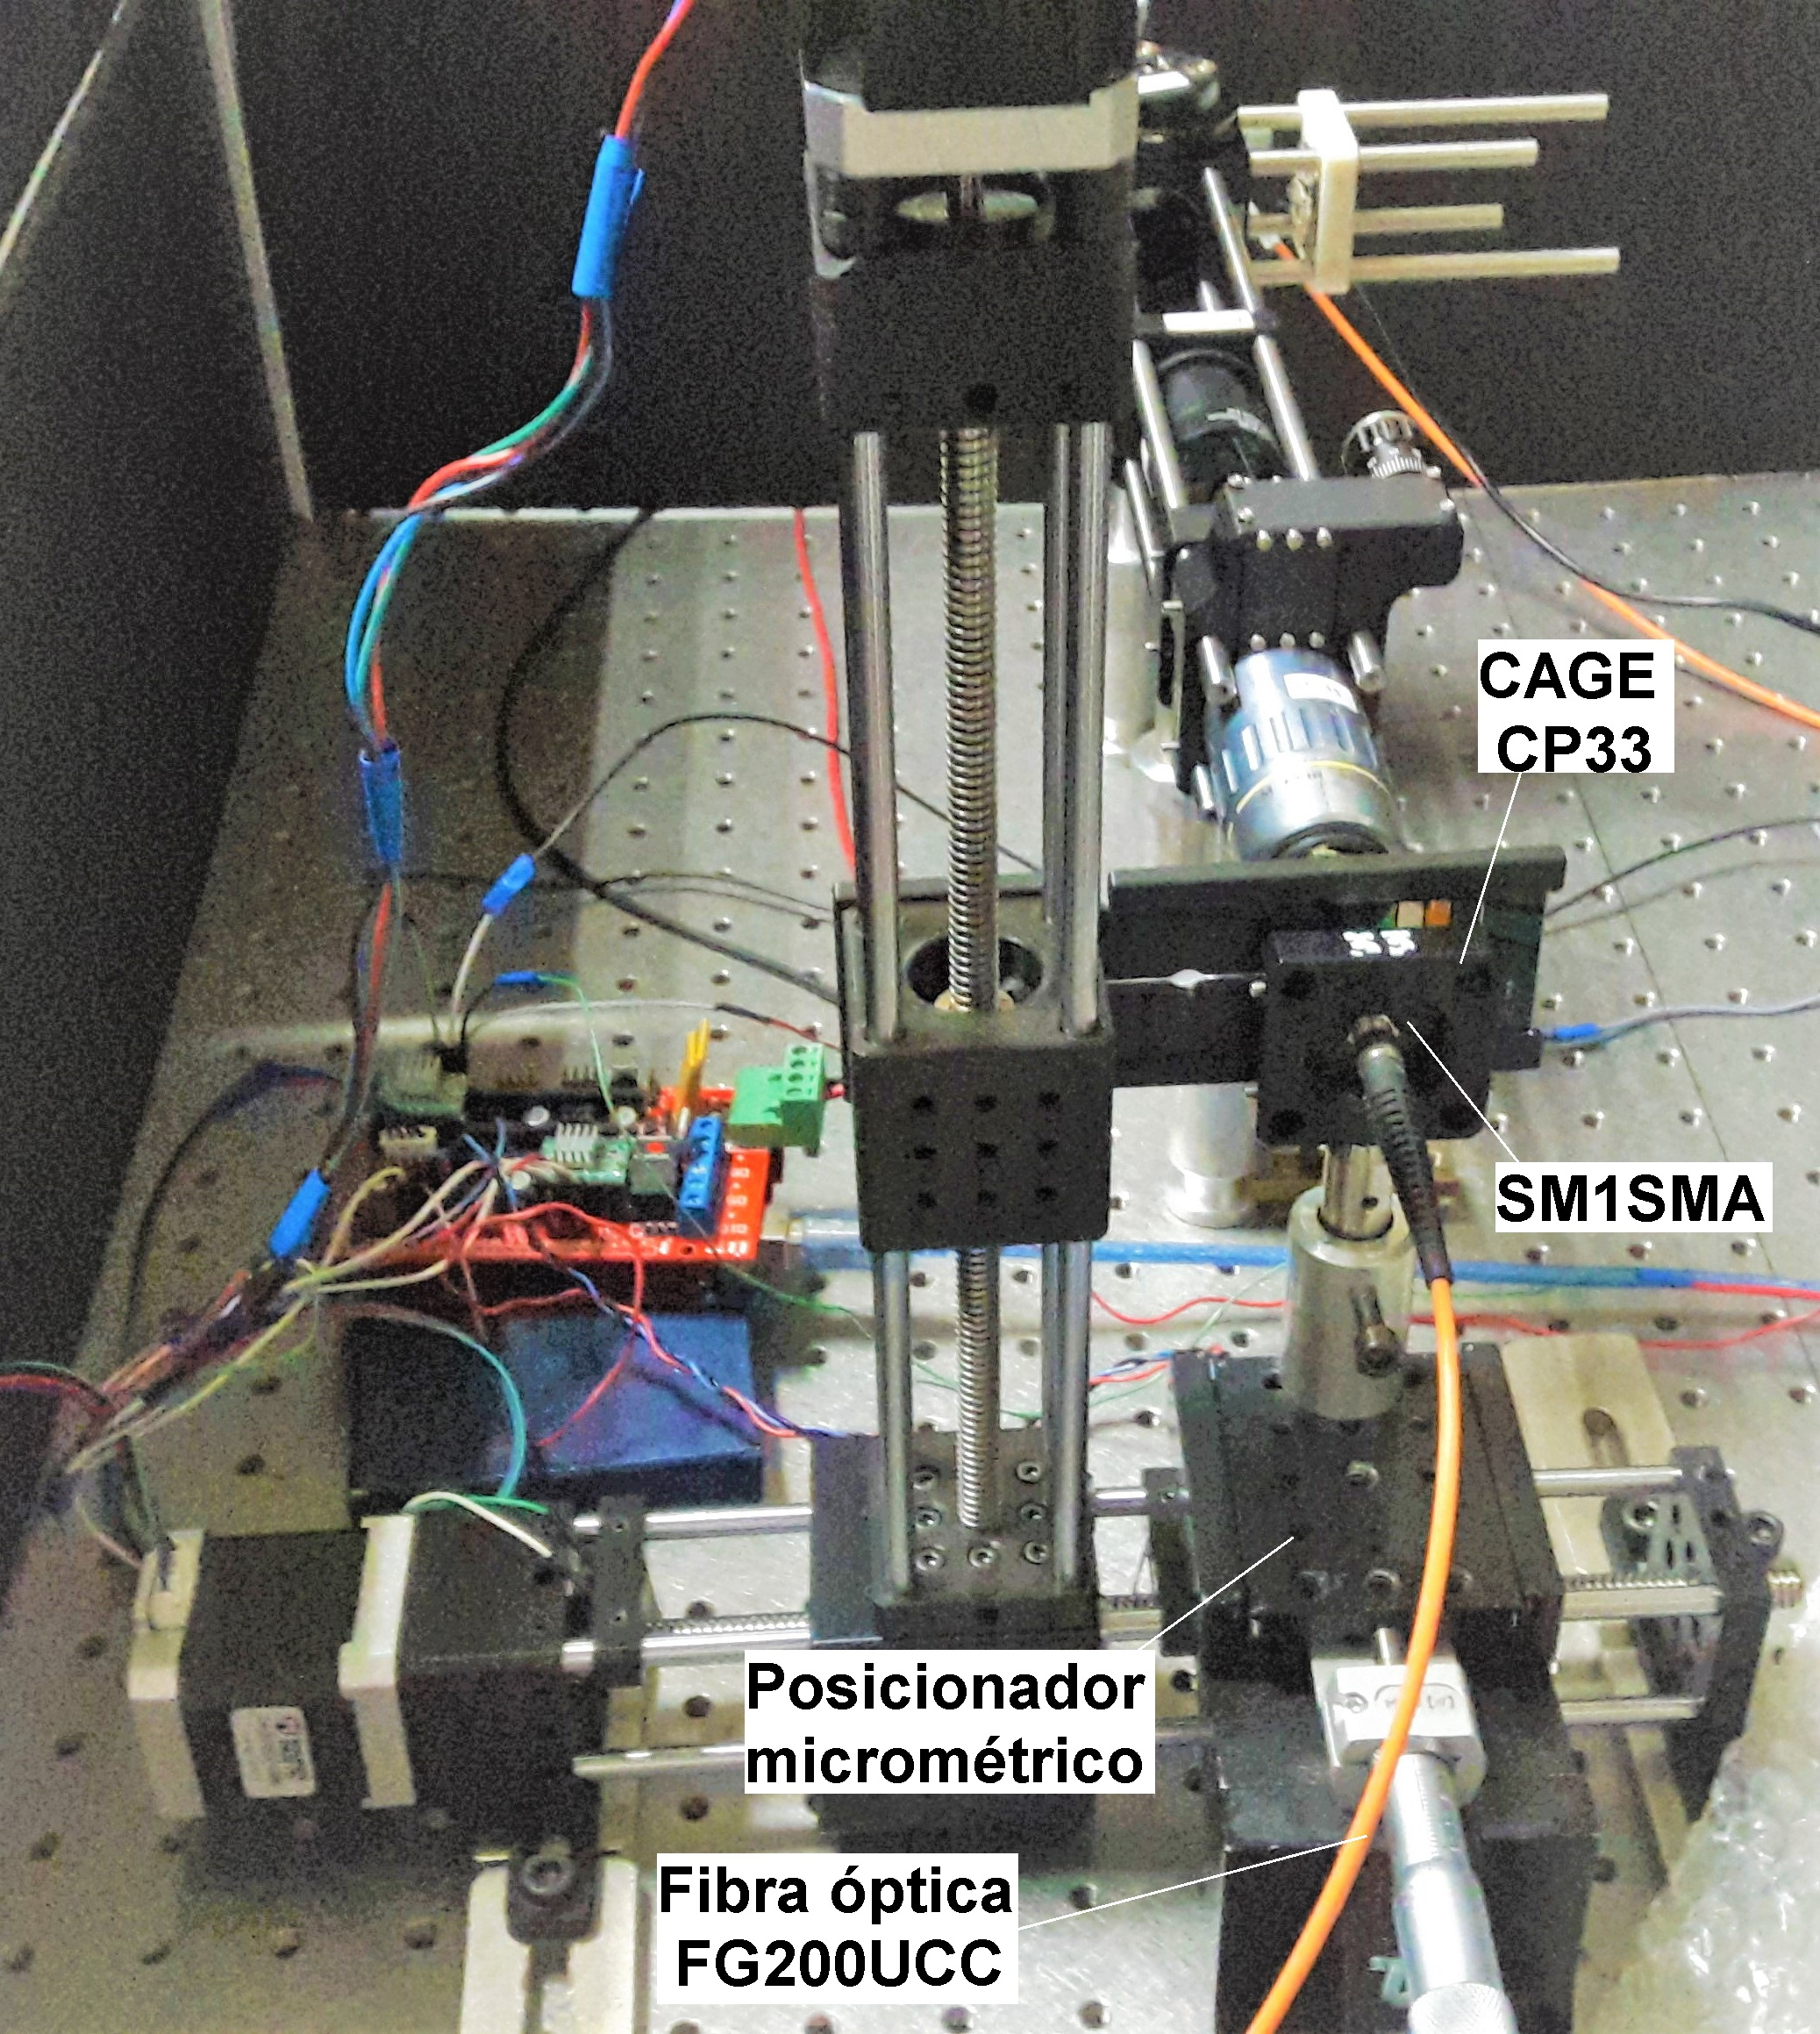
\includegraphics[scale=0.13]{Figs/microespectrometro/setupactualdecote_retoc_condetalles.jpg}
	\caption{Montaje de la fuente de luz.}
	\label{fig:montttluz}
\end{figure}


 
%%%%%%%%%%%%%%%%%%%%%%%%%%%%%%%%%%%%%%%%%%%%%%%%%%%%%%%%%%%%%%%%%%%%%%%%%%%%%%%%%%%%%%%%%%%%%%%%%%%%%%%%%%%%%%%%%%%%%%%%%%%%%%%%%%%%%%%%%%%%%%%%%%%%%%%%%%%%%%%%%%%%%%%%%%%%%%%%%%%%%%%%%%%%%%%%%%%%%%%%%%%%%%%%%%%%%%%%%%%%


\singlespacing
\subsection{Platina \href{https://github.com/jrr1984/open\_frame\_XYStage}{\faGithub$_{3.2.2}$} \href{https://github.com/jrr1984/open\_frame\_XYStage/tree/master/3dprintedparts/STLs}{\faCubes}}
\label{sec:platina}
\spacing{1.5}

\hspace{0.5cm}Se desarrolló una platina de microscopía con dos grados de libertad para poder desplazar el filtro lateral y verticalmente respecto de la fuente de luz y del microespectrómetro para poder medir el espectro de transmisión del filtro en distintas regiones del mismo. Una imagen representativa de una de las primeras versiones de la platina con dos grados de libertad se muestra en la Figura \ref{fig:plato0}.


\begin{figure}[H]
	\centering
	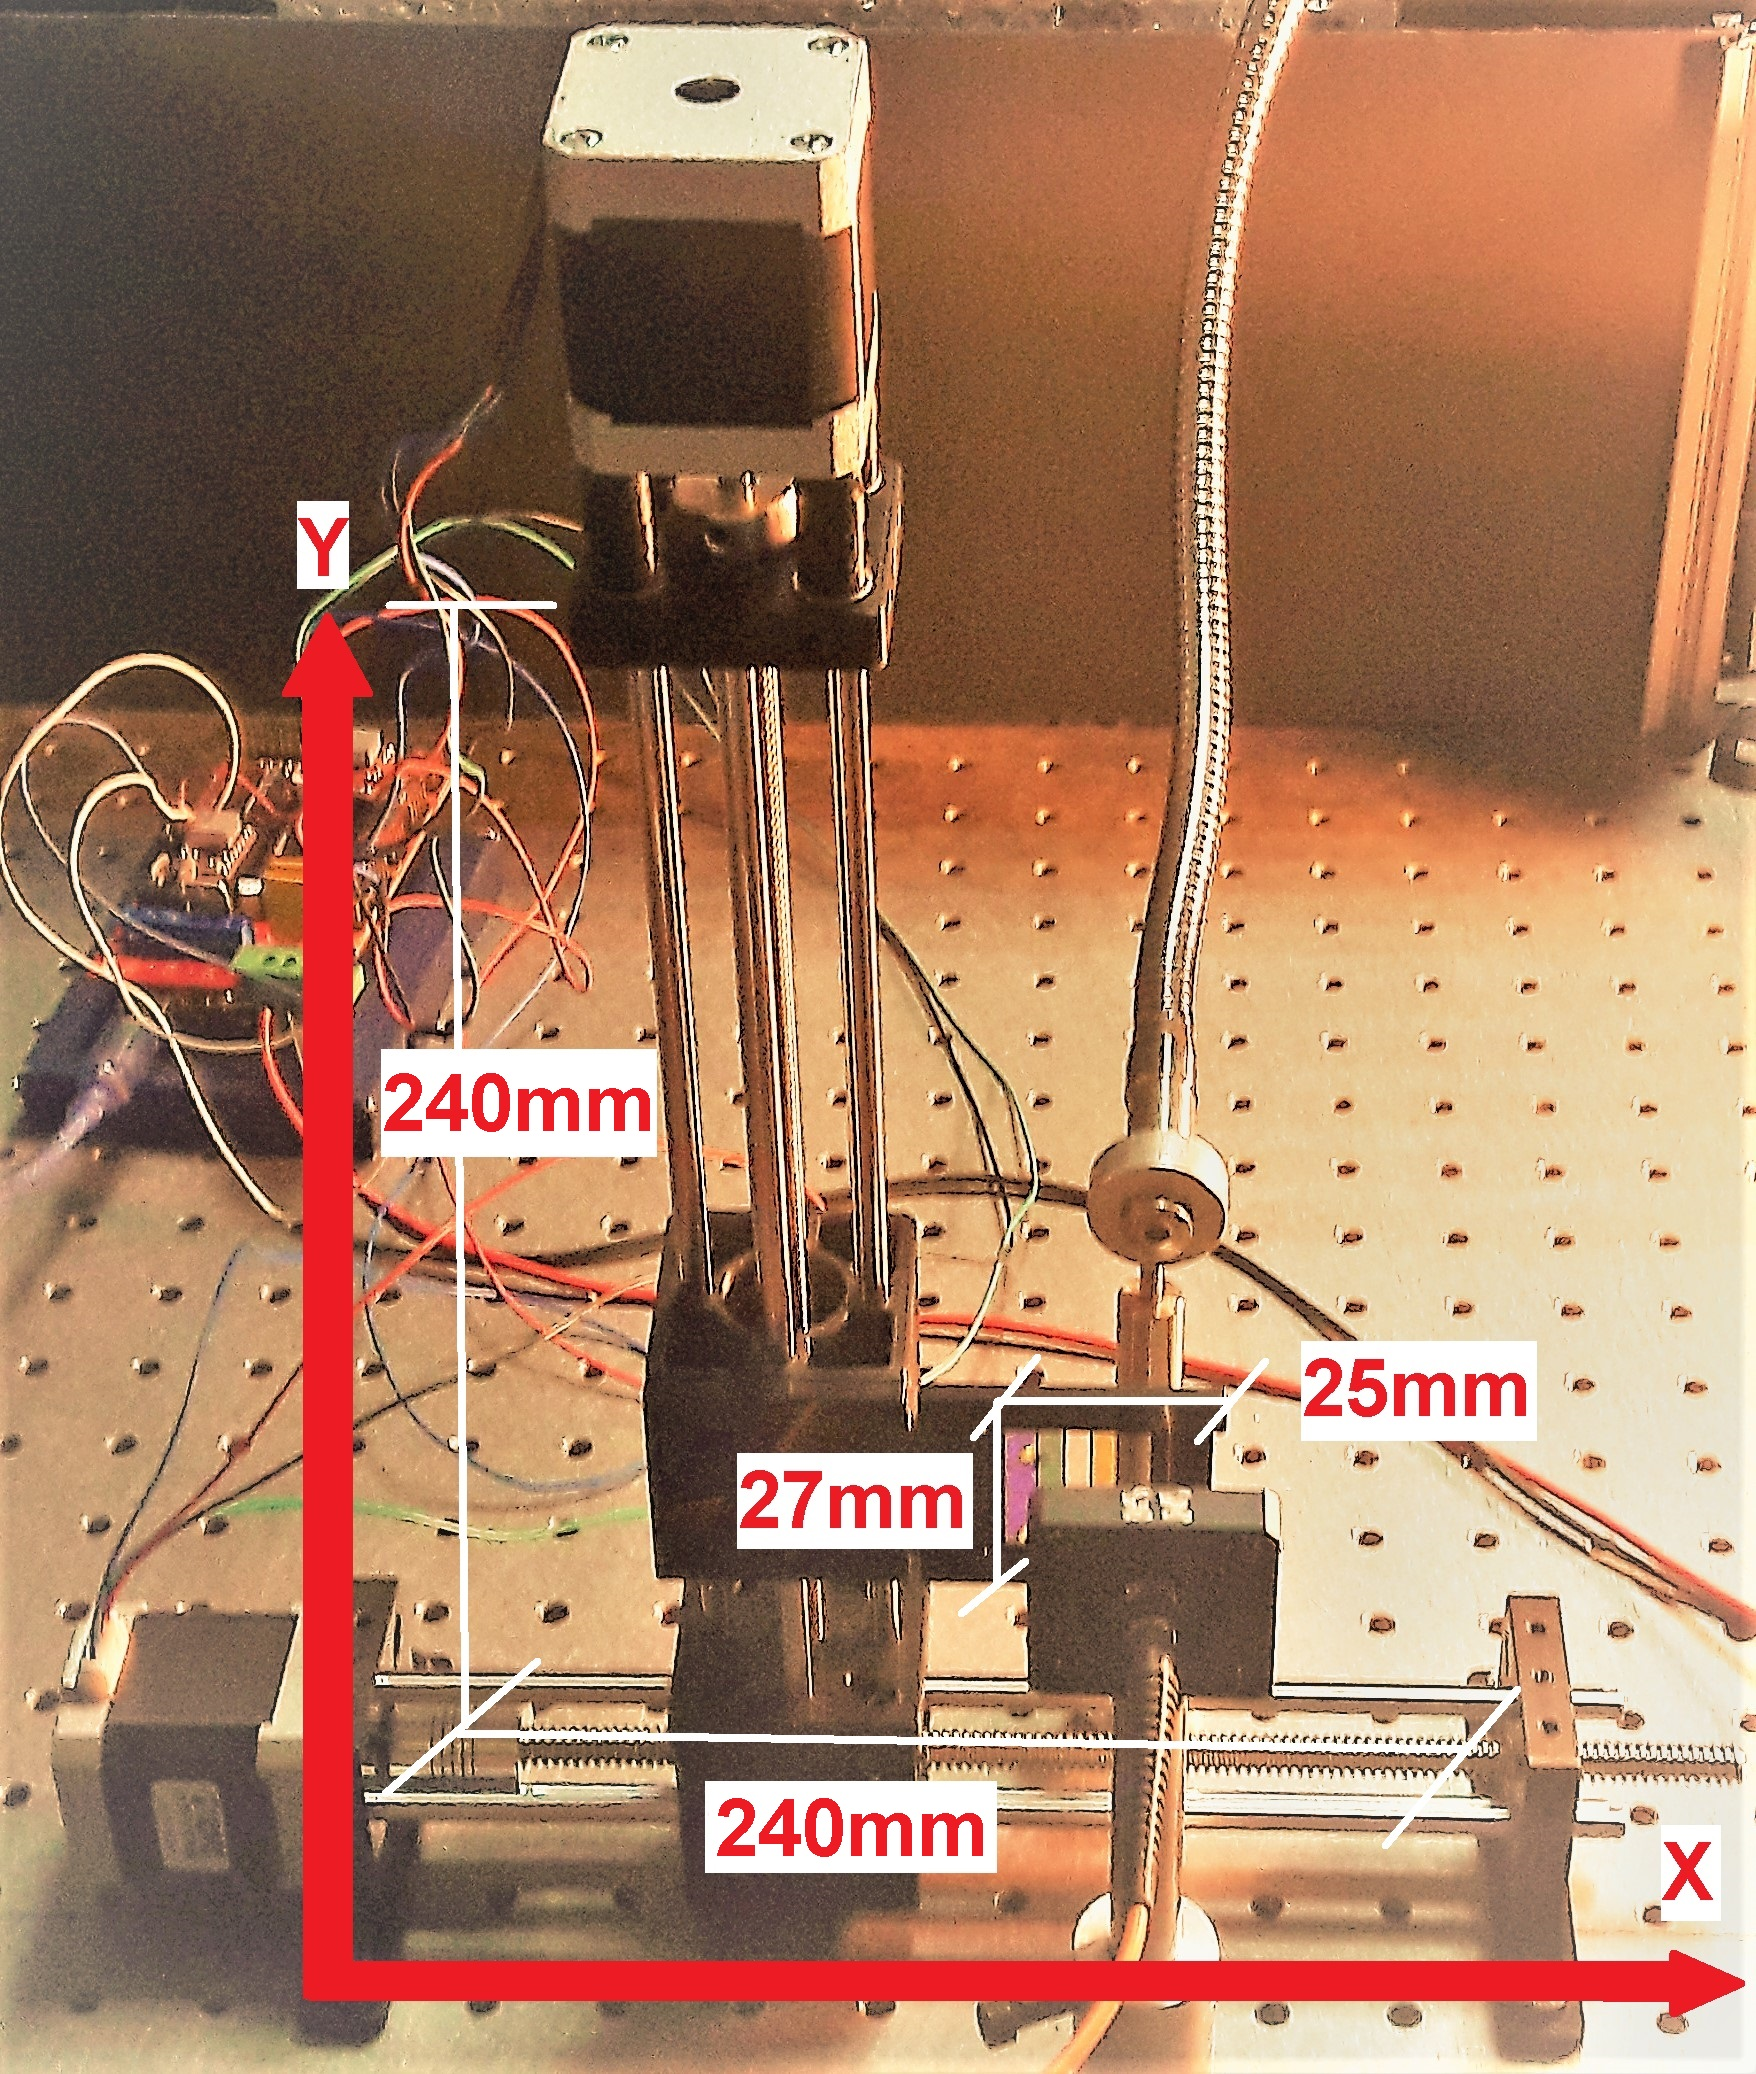
\includegraphics[scale=0.16]{Figs/microespectrometro/stageearly.jpg}
	\caption{Imagen de una de las primeras versiones de la platina motorizada con dos grados de libertad.}
	\label{fig:plato0}
\end{figure}


La construcción y desarrollo de la platina motorizada del microespectrómetro consistió de las siguientes etapas de prototipado:

\begin{enumerate}
\item Investigación previa de la literatura sobre platinas de microscopía de bajo costo y factibles para integrar al prototipo.
\item Elección de los componentes y materiales en función de la oferta local en Argentina.
\item De acuerdo al ítem 2, se realizó un dimensionamiento de la platina y se determinó el recorrido total de cada uno de los grados de libertad. Esto permitió evaluar la factibilidad y aplicabilidad de la plataforma a desarrollar.
\item En conjunto con el diseñador industrial Federico Armesto se diseñaron las piezas de impresión 3D y se montó el primer eje de la platina. Se desarrolló la electrónica y el \textit{software} necesarios.
\item Una vez optimizado el diseño del primer eje, se montó el segundo eje de la platina. Se extendió el software y se integraron finales de carrera.
\item Desarrollo del \textit{software} de control de la platina. Calibración preliminar.
\end{enumerate}

A continuación se describen algunas consideraciones técnicas y de diseño que se tuvieron en cuenta para el desarrollo de la platina motorizada y que podrían ser de utilidad para otros laboratorios que quisieran replicar la plataforma que aquí se presenta, realizar una adaptación ó simplemente como fuente de consulta.

Respecto de la revisión de la literatura sobre platinas de microscopía de bajo costo y factibles para el prototipo, se consultaron  los prototipos cuyos proyectos hayan sido desarrollados bajo la modalidad \textit{open source} tanto para la distribución del diseño de las piezas 3D como del \textit{software}, dentro de las cuales se destacan \cite{schaa}(\textit{LabView}, EUR 250) y \cite{campbells}(Instrucciones vía puerto serie en \textit{Matlab}, \textit{LabView} y \textit{python}, USD 1000). Dichas propuestas son también denominadas en cierto contexto DIY (\textit{Do it yourself}) ya que contienen toda la documentación y herramientas necesarias para que cualquier usuario con presupuesto y acceso a los mismos componentes pueda reproducir el proyecto. Además de estos proyectos se consultaron múltiples platinas de microscopía comerciales, donde en sus páginas la mayoría de los fabricantes distribuyen los planos de diseño, las piezas 3D libres para modificar, etc (\href{https://www.thorlabs.com/newgrouppage9.cfm?objectgroup\_id=2132}{NRT150 Thorlabs} USD 2456 x 2, \href{https://www.edmundoptics.com/p/150mm-motorized-stage/16419/}{\#59-747 EO} USD 2095 x 2). Ahora bien, hasta la fecha de escritura de este trabajo no se registraban prototipos de platinas motorizadas de microscopía desarrolladas en laboratorios del país como la que aquí se presenta por lo cual por medio de la presente se comparten las piezas de diseño 3D y el \textit{software} necesarios para poder replicarla y extender sus prestaciones. El costo total aproximado de la platina aquí desarrollada fue de USD 200.

El tipo de platina motorizada a desarrollar dependió del presupuesto, de la oferta local de los componentes y de los requerimientos mecánicos de precisión, longitud de recorrido y repetibilidad. Estos tres conceptos se encontraban relacionados fuertemente entre sí. Si bien se podrian haber comprado los componentes de la platina en el exterior del país, la futura necesidad de comprar nuevamente alguno de los componentes debido al desgaste ó rotura de los mismos, hacen de esta implementación de la compra una mala práctica del prototipado. En este sentido se eligieron componentes masivos en el país, los cuales se podían conseguir fácilmente sus repuestos en caso de necesidad. Al mismo tiempo, los componentes masivos son los que tienen un menor costo debido a su mayor demanda.

Se consultaron fundamentalmente tres proveedores de componentes mecánicos y de electrónica, de la ciudad de Buenos Aires y de la provincia de Buenos Aires: \href{https://3dinsumos.com.ar/}{3DInsumos} (Caseros, Buenos Aires), \href{https://ingia.com.ar/}{Ingia Automatización} (Saavedra, C.A.B.A.) y \href{https://candy-ho.com/}{Candy-Ho} (Villa Martelli, C.A.B.A.). A partir de la oferta de estos y otros proveedores se eligieron los componentes de la platina tomando como idea de diseño e implementación la platina de \cite{schaa} que por su bajo costo y la utilización de piezas 3D que facilitaban el prototipado rápido (dependiendo de la disponibilidad de una impresora 3D), hacían de esa propuesta la más indicada para ser implementada.

Los componentes principales de la platina son el motor paso a paso y el sistema de transmisión que transforma la rotación del motor en un desplazamiento lineal. Uno de los motores paso a paso más populares del mercado sino el más popular es el \href{https://www.pololu.com/product/1200}{NEMA 17} que es ampliamente utilizado en impresoras 3D y CNC. Por este motivo se eligió ese motor en lugar del \href{https://www.pololu.com/product/1204}{NEMA 8} utilizado en \cite{schaa}, que sólo se podía conseguir haciendo un pedido al exterior lo que encarece su costo y alarga notablemente los tiempos de prototipado.

De la familia de motores paso a paso NEMA 17 (Ver Figura \ref{fig:acm} (a)) existen distintos modelos dependiendo los requerimientos de torque y de resolución fundamentalmente. El torque no fue una limitante para la elección del modelo con lo cual en función de las distintas opciones de torque se priorizó el de menor precio. Ahora bien, respecto de la precisión existen dos modelos con pasos mínimos de rotación de 1.8 grados y de 0.9 grados, con lo cual se tienen 200 y 400 pasos por revolución respectivamente. Se evaluó la oferta disponible en el mercado y se eligieron motores NEMA 17 con un paso mínimo de 0.9 grados con el fin de obtener la mayor resolución en el desplazamiento lineal, a pesar de que su costo era mayor.

A la elección del motor, le sigue la elección del sistema de transmisión donde existen múltiples opciones dependiendo de la precisión, entre ellas las correa dentadas con poleas, las varillas roscadas, los husillos de bolas, etc. De acuerdo a \cite{schaa} se optó por una varilla roscada masiva en el mercado del tipo \href{https://www.mcmaster.com/acme-screws/acme-lead-screws-and-nuts/}{ACME} (Ver Figura \ref{fig:acm} (b)) de un diámetro de 8 mm y con un paso (\textit{pitch}) de 2 mm, es decir que por cada revolución completa del motor se realiza un desplazamiento lineal de 2 mm. La rotación del motor paso a paso es transferida a la varilla roscada ACME por medio de un acople sólido con agujeros para prisioneros M3 equidistanciados a 180° para que la varilla roscada quede centrada, que fue diseñado (Ver \href{https://github.com/jrr1984/open\_frame\_XYStage/blob/master/3dprintedparts/STLs/acopleRIGIDO.STL}{\faCubes$_{1}$}).
\begin{figure}[H]
%\centering
\hfill%
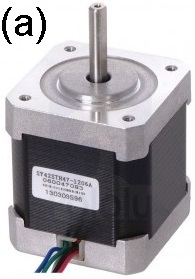
\includegraphics[scale=0.7]{Figs/microespectrometro/nema17.jpg}
\hfill%
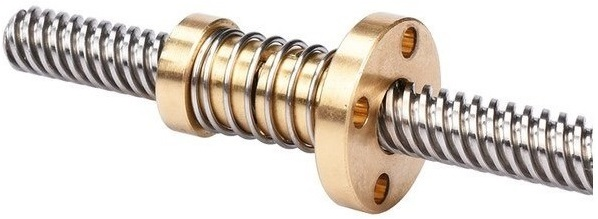
\includegraphics[scale=0.7]{Figs/microespectrometro/acmeantib.jpg}
\hfill%
\hfill%
\caption{(a) Motor paso a paso \href{https://www.pololu.com/product/1200}{NEMA 17} con una resolución de 400 pasos por revolución (0.9° por paso). (b) Varilla roscada del tipo \href{https://www.mcmaster.com/acme-screws/acme-lead-screws-and-nuts/}{ACME} con un paso (\textit{pitch}) de 2 mm  y un diámetro de 8 mm, junto con una tuerca \textit{anti-backslash}.}
\label{fig:acm}
\end{figure}

Además del sistema de transmisión se tuvo que elegir un sistema de desplazamiento que es el que permite el movimiento de los ejes de la platina. Se eligió la opción más utilizada en impresoras 3D en el que se utilizan sistemas lineales con barras rectificadas de acero de 6mm de diámetro y rodamientos lineales \href{https://uk.misumi-ec.com/vona2/detail/221000091678/?HissuCode=LM6LUU}{LM6LUU}. Dichos rodamientos y la tuerca \textit{antibackslash} fueron montados sobre un cubo diseñado e impreso con una impresora 3D (Ver \href{https://github.com/jrr1984/open_frame_XYStage/blob/master/3dprintedparts/STLs/cuboconLM6UU_2demarzo.STL}{\faCubes$_{2}$}) que realizó los desplazamientos lineales al deslizarse sobre las barras de acero.

La resolución espacial mecánica es el mínimo desplazamiento de cada uno de los ejes de la platina. La misma viene dada teóricamente por la siguiente ecuación:
\begin{equation}
\text{Resolución} [\mu m / paso] = \frac{\text{\textit{Pitch} del ACME}}{\text{\# de pasos por revolución del motor}} = \frac{2 mm}{400 pasos} = \frac{5 \mu m}{paso}
\end{equation}

Además esta resolución fue modificada por medio de la electrónica que controla los motores paso a paso implementando una técnica que se conoce como \textit{microstepping} \cite{7806244}. Esta técnica permite al motor realizar rotaciones de ángulos menores al paso mínimo del motor, con lo cual se mejora la resolución ya que se puede subdividir un paso completo del motor en 2,4,8,16 e incluso hasta en 32 pasos (teóricos). Al mismo tiempo se reduce el ruido del motor y el movimiento del mismo se suaviza. La técnica es impelementada por el controlador de corriente que utiliza un algoritmo que a su salida envía una modulación sinusoidal discretizada de la corriente, donde cada paso de dicha modulación sinusoidal consiste de un micropaso y el período de la señal es igual al paso completo original del motor.

Los dos controladores de corriente de los motores paso a paso más populares con la capacidad de aplicar \textit{microstepping} son el \href{https://www.pololu.com/product/2133}{DRV8825}(hasta 32 micropasos y 2.5 A) y el \href{https://www.pololu.com/product/1182}{A4988} (hasta 16 micropasos y 2 A). Se eligió finalmente para la platina el \textit{driver} A4988 (Ver Figura \ref{fig:elec} (a)) y se limitó la máxima corriente que podía entregar de acuerdo al consumo observado de los motores en condiciones de operación normales, ajustando el potenciómetro (Ver Figura \ref{fig:elec} (a)) a partir de la medición de una tensión de referencia de acuerdo a las especificaciones del manual del fabricante \cite{a4988}.

\begin{figure}[H]
%\centering
\hfill%
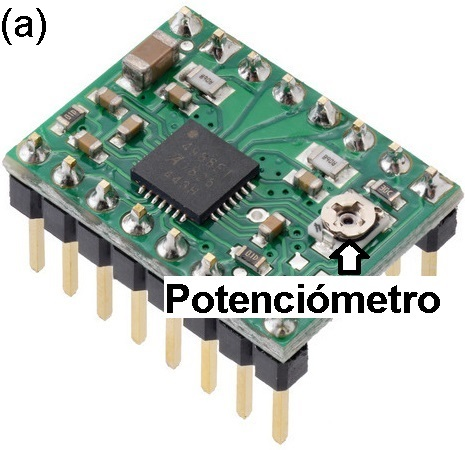
\includegraphics[scale=0.3]{Figs/microespectrometro/a4988.jpg}
\hfill%
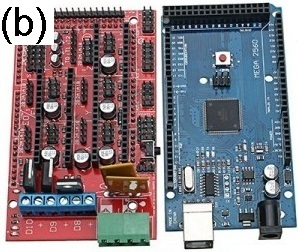
\includegraphics[scale=0.8]{Figs/microespectrometro/megaramps.jpg}
\hfill%
\hfill%
\caption{(a) Controlador de los motores paso a paso A4988. (b) \href{https://store.arduino.cc/usa/mega-2560-r3}{\textit{Arduino MEGA 2560}} a la derecha en azul y \href{https://reprap.org/wiki/RAMPS_1.4}{\textit{Shield RAMPS 1.4}} a la izquierda en rojo.}
\label{fig:elec}
\end{figure}

Se utilizó un \href{https://store.arduino.cc/usa/mega-2560-r3}{\textit{Arduino MEGA 2560}} para controlar la lógica de la platina vía el puerto USB de una computadora y se le montó a los pines hembra del arduino un \textit{shield} \href{https://reprap.org/wiki/RAMPS_1.4}{\textit{RAMPS 1.4}} donde se colocaron los \textit{drivers} de los motores, las conexiones de los finales de carrera y el \textit{joystick} (Ver Figura \ref{fig:elec} (b)). La RAMPS fue alimentada de forma independiente con una fuente de tensión.

Antes de realizar la compra de los componentes necesarios para montar el primer eje se determinó el recorrido total de cada uno de los grados de libertad de la platina de acuerdo a la oferta de los proveedores. Por ejemplo, existen comercialmente distintas longitudes de varillas roscadas ACME y se eligió una longitud de la misma de 500 mm, de forma tal que al cortar dicha varilla se pueda obtener las dos varillas necesarias para cada eje de la platina, cada una de 250 mm de largo. El mismo razonamiento fue aplicado a las varillas de acero de 6 mm de diámetro, para las cuales se compraron dos varillas de 1 metro que cada una fue cortada en cuatro partes de 250 mm cada una. De esta manera, se realizó un diagrama con las dimensiones y la longitud de recorrido estimada de uno de los ejes de la platina con el software \textit{Solidworks} como se muestra en la Figura \ref{fig:dimejee}.

\begin{figure}[H]
	\centering
	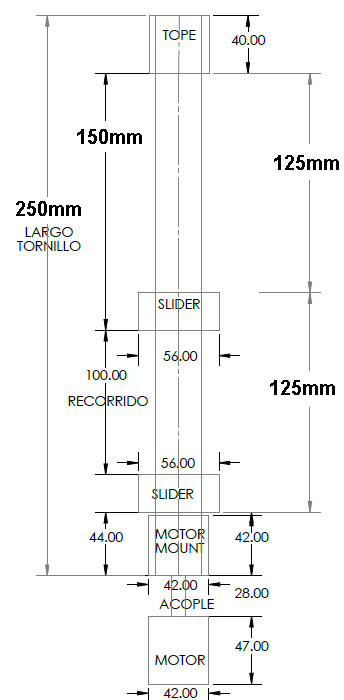
\includegraphics[scale=0.9]{Figs/microespectrometro/dimensio.png}
	\caption{Estimación del recorrido de uno de los ejes de la platina.}
	\label{fig:dimejee}
\end{figure}

El objetivo de esta etapa del prototipado fue el de evaluar la factibilidad y aplicabilidad de la platina para poder desplazar al filtro respecto de la fuente de luz y del espectrómetro de manera tal de poder obtener una medición del espectro en cualquier región del filtro deseada. Luego de realizar el dimensionamiento, se decidió montar el eje $\textit{x}$ de la platina únicamente. En la Figura \ref{fig:dis} (a) se muestra el diseño del eje $\textit{x}$ realizado con el software libre \textit{Fusion 360} y en la Figura \ref{fig:dis} (b) se muestra un montaje preliminar de dicho eje\footnote{Se imprimió inicialmente una porción del cubo diseñado como prueba preliminar, ya que la impresión del cubo completa podía tomar más de 10 horas. Resultó importante realizar pruebas por etapas para reducir los tiempos de prototipado.}. 

\begin{figure}[H]
%\centering
\hfill%
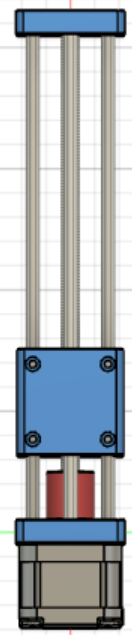
\includegraphics[scale=0.83]{Figs/microespectrometro/diseo1eje.png}
\hfill%
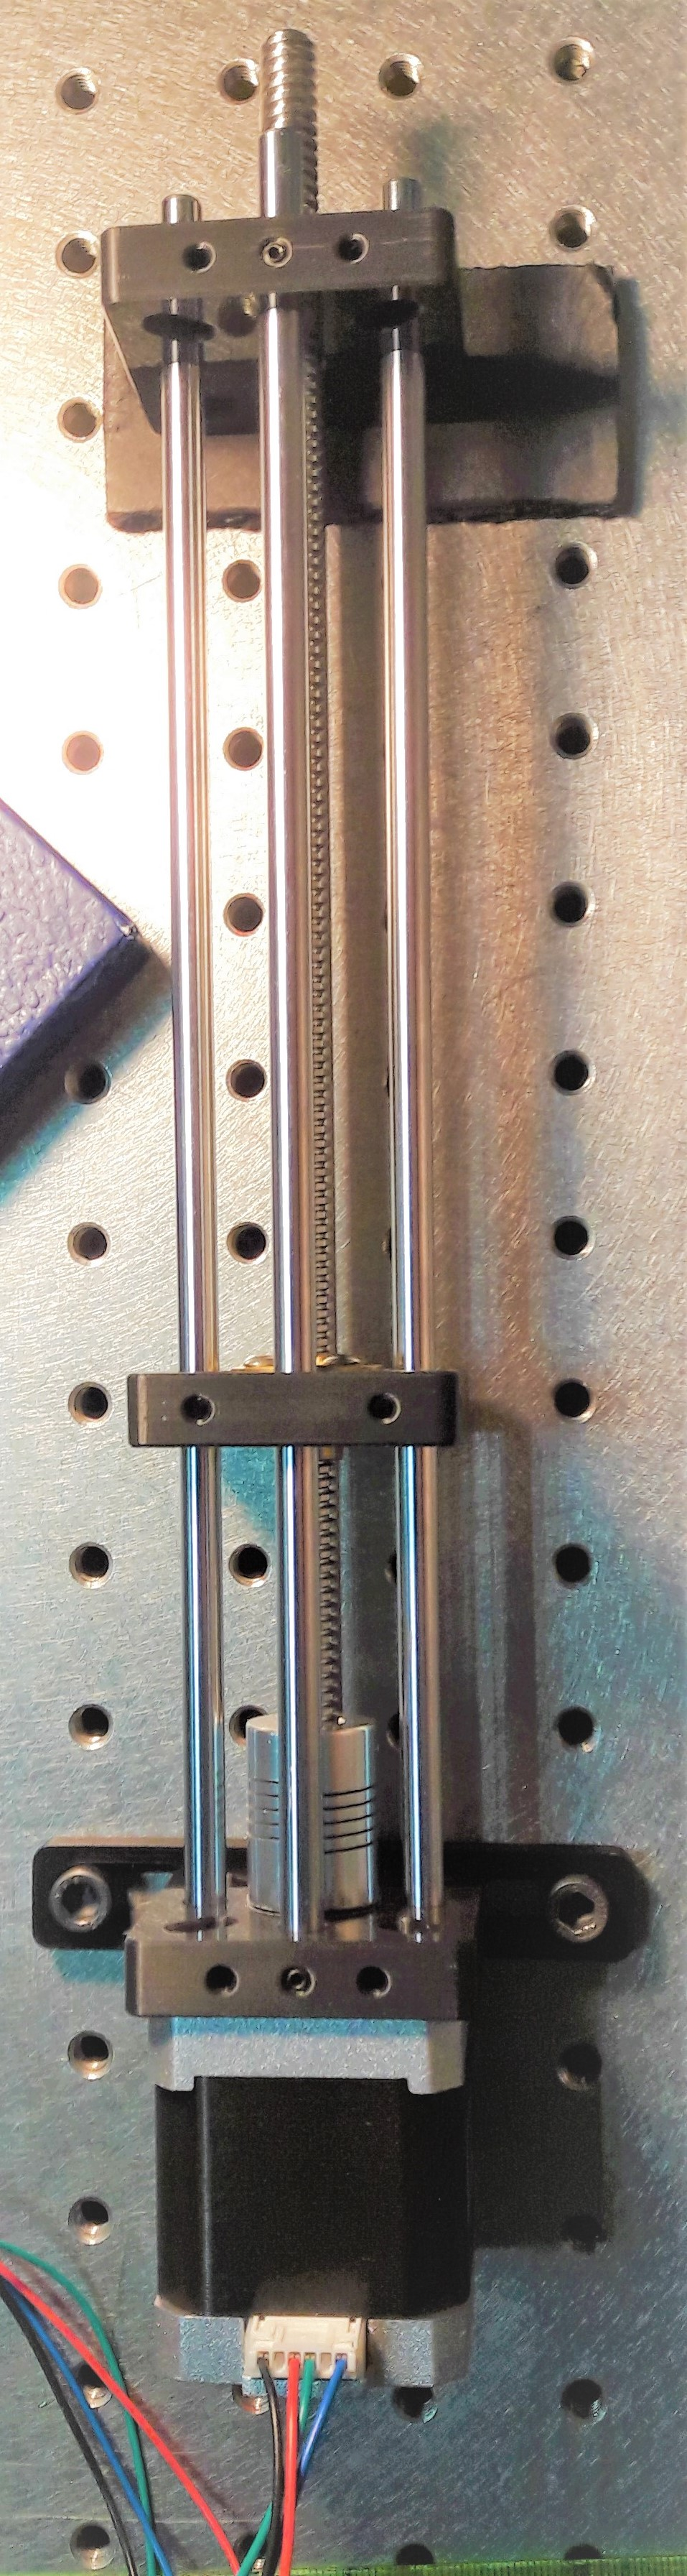
\includegraphics[scale=0.073]{Figs/microespectrometro/1ejemontado.jpg}
\hfill%
\hfill%
\caption{(a) Diseño de las piezas 3D del eje $\textit{x}$ de la platina [\href{https://github.com/jrr1984/open_frame_XYStage/blob/master/3dprintedparts/STLs/Ejexpreliminar.stl}{\faCubes$_{3}$}]. (b) Montaje preliminar del eje $\textit{x}$ de la platina.}
\label{fig:dis}
\end{figure}


Luego de optimizar el diseño y montaje del primer eje, se montó el eje $\textit{y}$ compuesto por las mismas piezas 3D que el eje $\textit{x}$, como se muestra en la Figura \ref{fig:2e}. En este sentido se hace notar que el diseño propuesto resultó una solución completamente modular y que la configuración de los ejes aquí adoptada puede ser modificada a otras de acuerdo a las necesidades del usuario final. 
 
\begin{figure}[H]
%\centering
\hfill%
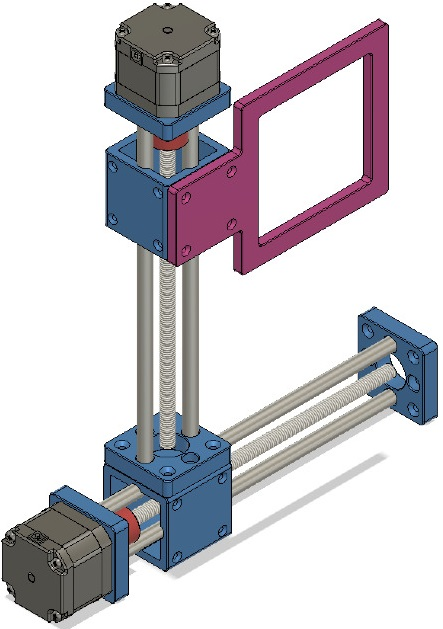
\includegraphics[scale=0.83]{Figs/microespectrometro/scanningstage.jpg}
\hfill%
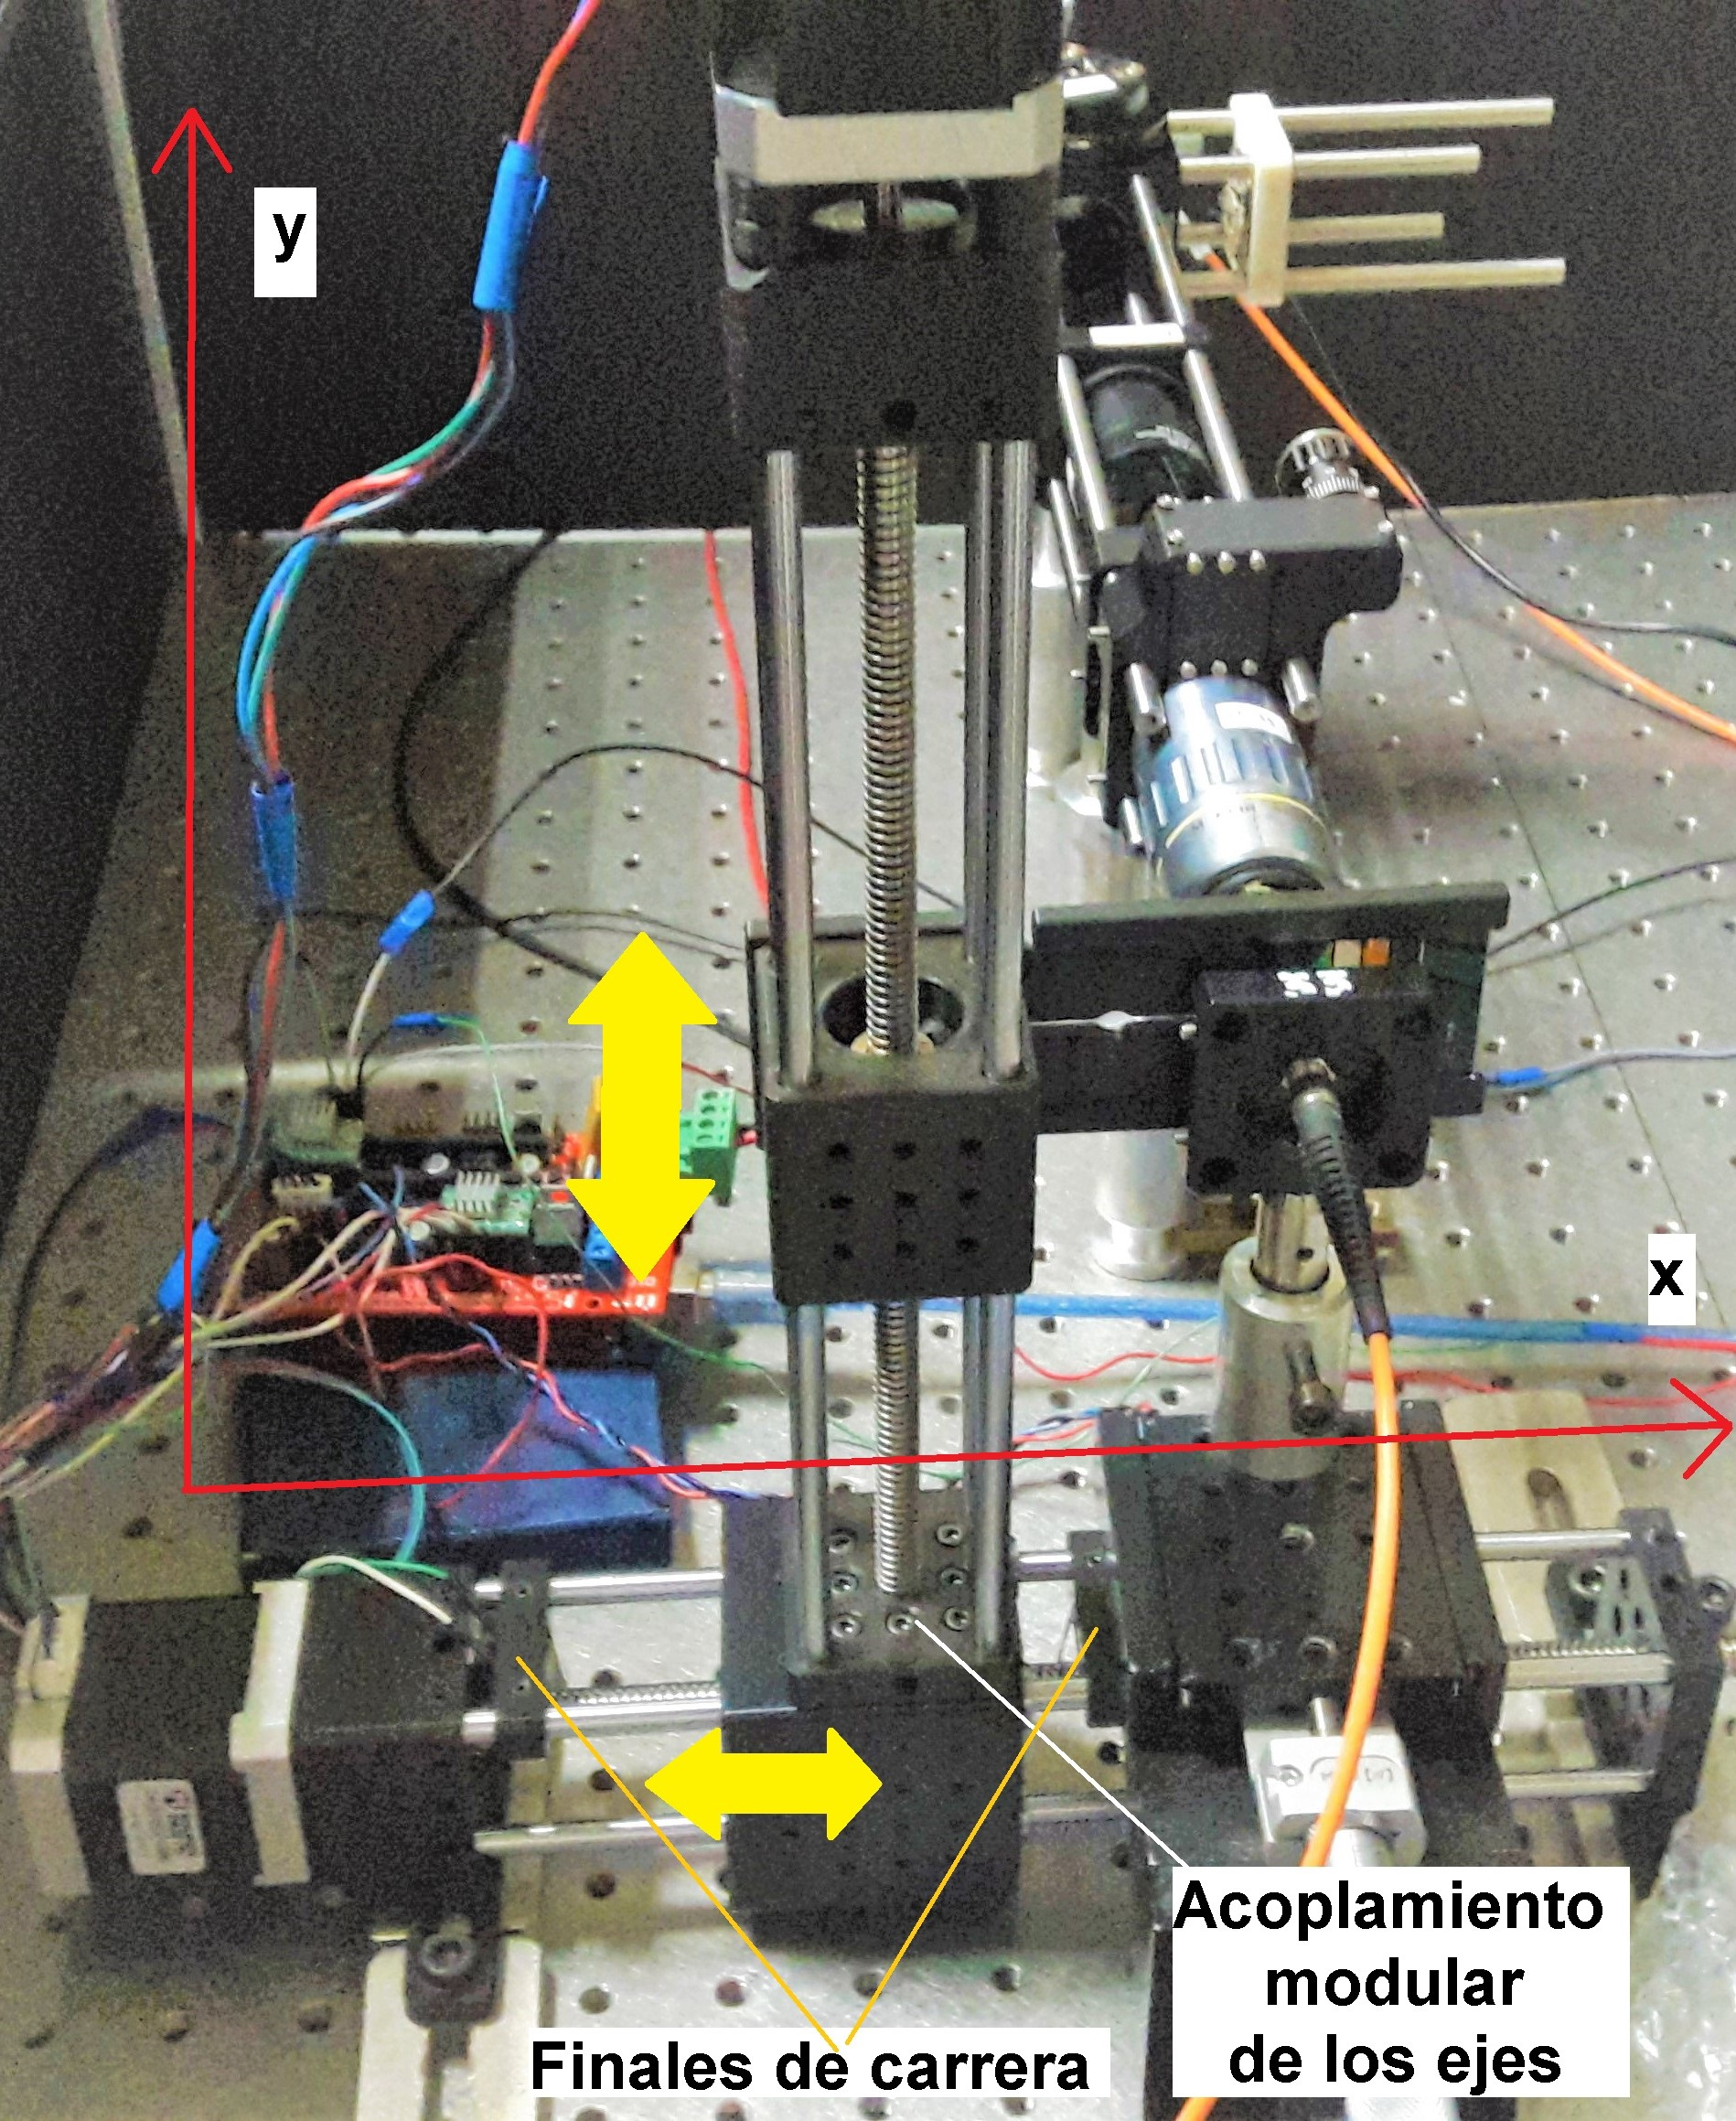
\includegraphics[scale=0.13]{Figs/microespectrometro/2ejesmontaje.jpeg}
\hfill%
\hfill%		
\caption{(a) Diseño preliminar de los dos ejes de la platina. (b) Montaje final de la de la platina.}
\label{fig:2e}
\end{figure}

%%%%%%%%%%%%%%%%%%%%%%%%%%%%%%%%%%%%%%%%%%%%%%%%%%%%%%%%%%%%%%%%%%%%%%%%%%%%%%%%%%%%%%%%%%%%%%%%%%%%%%%%%%%%%%
%%%%%%%%%%%%%%%%%%%%%%%%%%%%%%%%%%%%%%%%%%%%%%%%%%%%%%%%%%%%%%%%%%%%%%%%%%%%%%%%%%%%%%%%%%%%%%%%%%%%%%%%%%%%%%

\singlespacing
\subsubsection{\textit{Software} de control de la platina \href{https://github.com/jrr1984/open\_frame\_XYStage}{\faGithub}$_{3.2.2}$  y calibración preliminar}
\label{sec:softcalib}
\spacing{1.5}

\hspace{0.5cm}Se desarrolló un \textit{software} de control de la platina que fue integrado al \textit{software} de control del espectrómetro y de la cámara. En [\cite{campbells},\href{https://github.com/raacampbell/openstage/tree/master/serialInterfaceScripts}{\faGithub$_{3.2.2.2}$}] se desarrollaron instrucciones específicas de comandos a ejecutar vía el puerto serie al que se conectó el arduino que controla la lógica de la platina, por medio de los lenguajes de programación \textit{Matlab}, \textit{LabView} y \textit{python}. En el proyecto \textit{open source} \href{https://www.youtube.com/watch?v=Lm8oprDhAnQ}{RDL} [\href{https://forum.arduino.cc/index.php?topic=469343}{\faCode}] se desarrolló un \textit{software} de comandos muy exhaustivo a ejecutar únicamente por el puerto serie de arduino.

El \textit{software} de control de la platina fue organizado como se muestra en la Figura \ref{fig:cnpl}. A nivel del microcontrolador las instrucciones a los \textit{drivers} que regulan la corriente de los motores y le envían los pulsos PWM para que realicen la cantidad de pasos elegidos fueron desarrolladas con la librería de \textit{Arduino} \href{https://www.airspayce.com/mikem/arduino/AccelStepper/}{AccelStepper}. Dichas instrucciones escritas en el lenguaje de programación propio de arduino incluyen métodos para asignarle las posiciones de los motores, para leer las posiciones de los motores, para prenderlos, apagarlos, determinar si llegaron a la posición asignada ó no, para ponerlos en la posición inicial de la platina, para leer los finales de carrera, etc. Todos los métodos escritos se pueden ver en el \textit{header} del \textit{driver} desarrollado [\href{https://github.com/jrr1984/open_frame_XYStage/tree/master/ino_main}{\faGithub$_{3.2.2.3}$}].
Ahora bien, para poder integrar el control de la platina con el espectrómetro y con la cámara se tuvo que establecer una comunicación por medio de mensajes a través del puerto serie de la computadora. Para ello se utilizó la librería \href{https://github.com/kroimon/Arduino-SerialCommand}{\textit{SerialCommand}} que permitió unir la lógica a nivel del microcontrolador del \textit{Arduino} con la lógica a nivel del procesador de la computadora. De esta manera, en el lenguaje de programación \textit{python} se escribió una clase [\href{https://github.com/jrr1984/open\_frame\_XYStage/blob/master/XYStage.py}{\faGithub$_{3.2.2.4}$}] con los mismos métodos de control de la platina escritos con la librería \textit{AccelStepper} en \textit{Arduino} de forma tal de enviar mensajes al puerto serie de la computadora que el \textit{Arduino} se encontraba constantemente escuchando. Así por ejemplo, desde \textit{python} se envía un mensaje al puerto serie para mover el motor del eje $\textit{x}$ una distancia de 2 mm, el \textit{Arduino} escucha ese mensaje y le envía los pulsos PWM al motor para realizar el desplazamiento. En la Sección \ref{sec:softadq} se explica el \textit{software} desarrollado para automatizar las mediciones que integró el control de la platina con el espectrómetro y la cámara.

\begin{figure}[H]
	\centering
	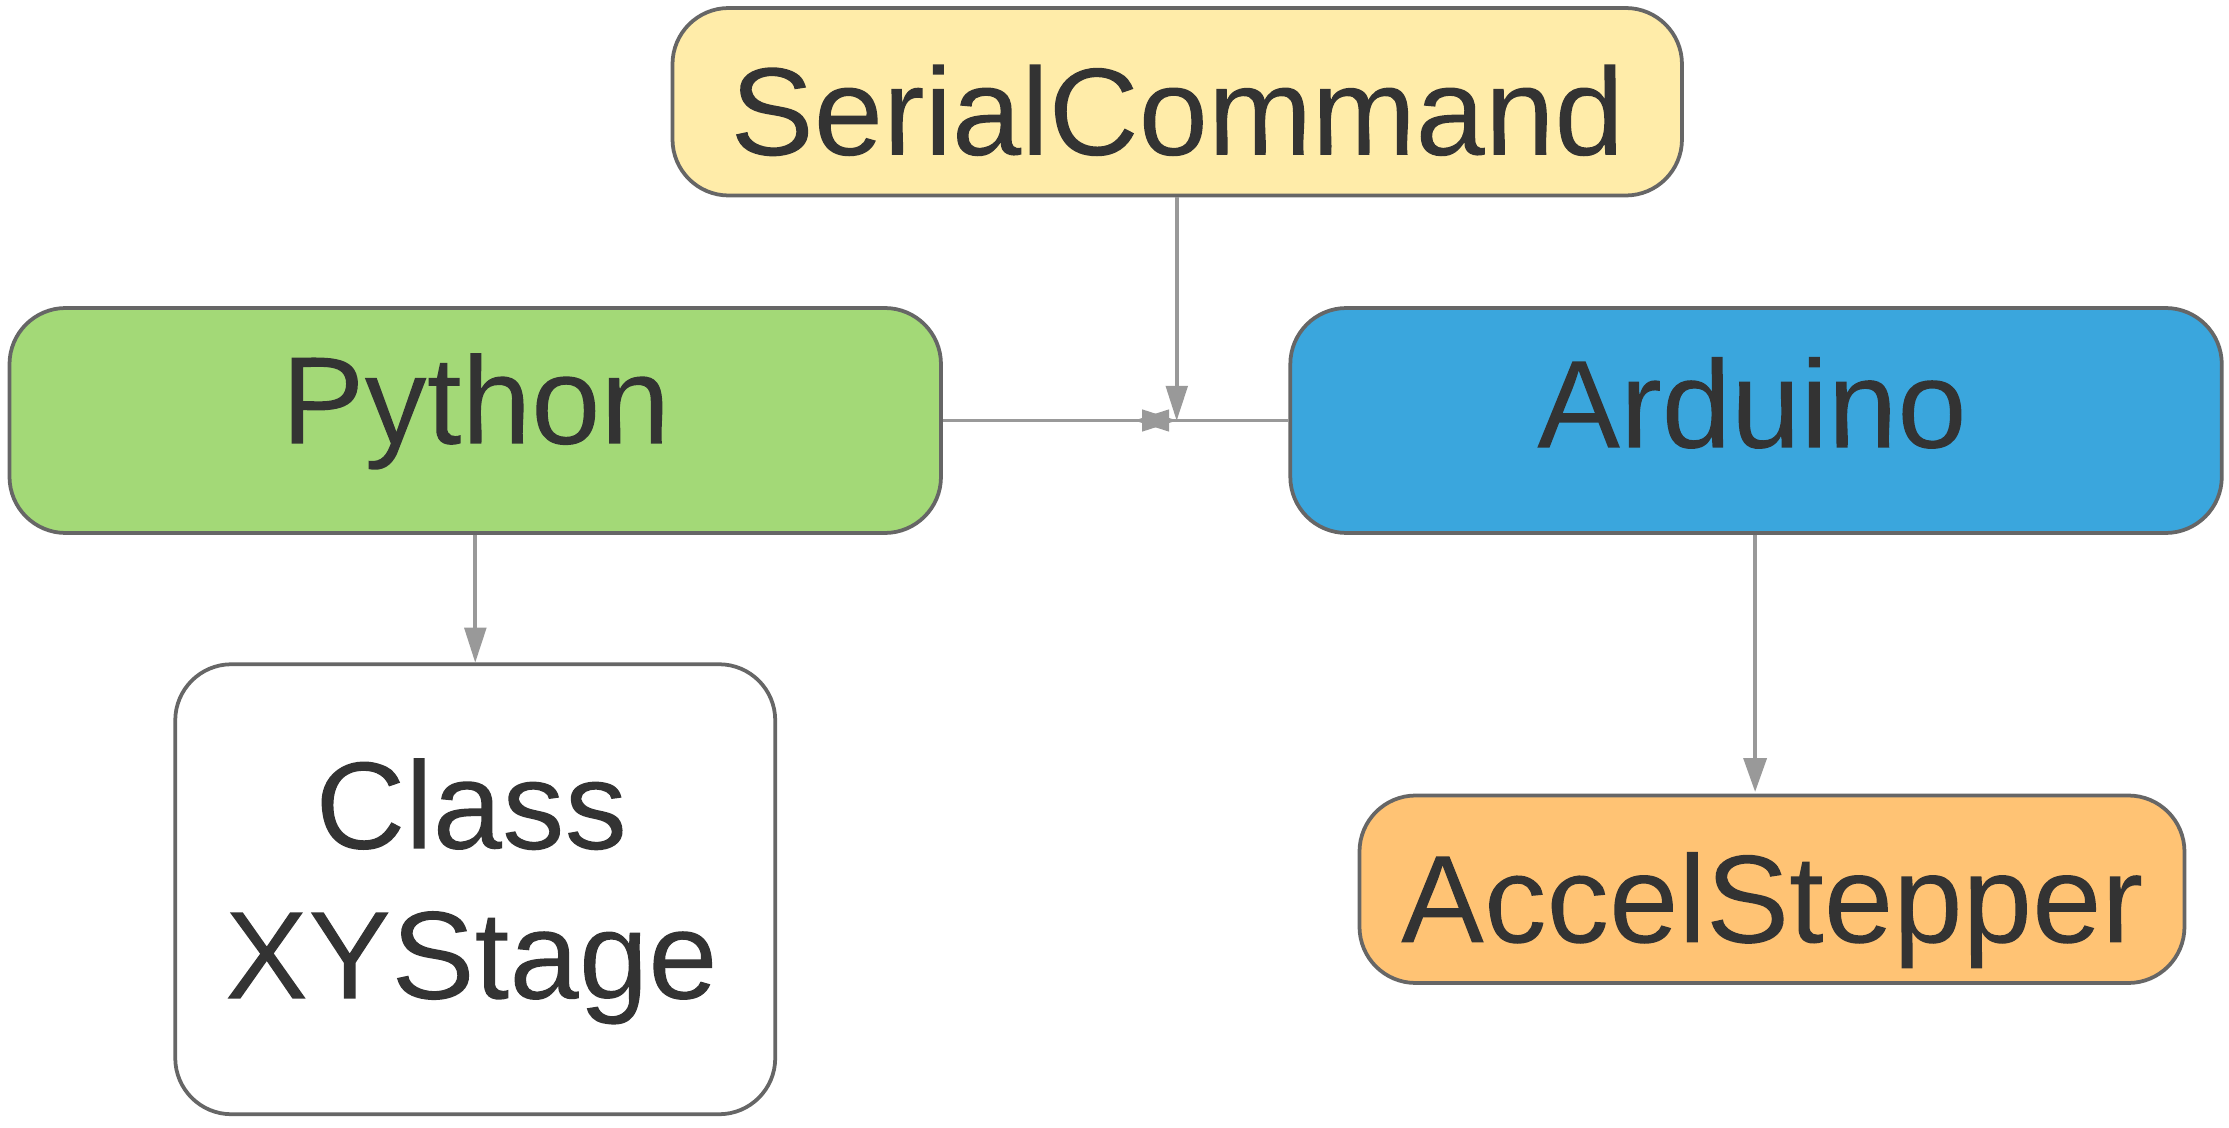
\includegraphics[scale=0.5]{Figs/microespectrometro/diagflujoplatina.png}
	\caption{Diagrama de la comunicación vía el puerto serie de la computadora entre el microcontrolador \textit{Arduino} y el proceso principal de la computadora programado en \textit{python} en el que se integró el espectrómetro y la cámara.}
	\label{fig:cnpl}
\end{figure}

Se realizó una calibración preliminar de la platina para determinar las incertezas de su resolución (mínimo paso de desplazamiento) que fueron luego utilizadas en la medición de la resolución espacial del microespectrómetro (Ver Sección \ref{sec:focoresol}). En el trabajo de \cite{schaa} realizaron una calibración de la platina adquiriendo sucesivas imágenes de una muestra calibrada de distancias (1951 USAF \textit{test target}), midiendo el desplazamiento relativo respecto de un punto de referencia situado en la imagen inicial adquirida. Al momento de escribir esta tesis se iba a realizar la calibración con el mismo método. El \textit{software} de adquisición ya se había desarrollado [\href{https://github.com/jrr1984/defectsGUI/blob/master/views.py}{\faGithub$_{3.2.4.2}$}] y ya se contaba con una pieza 3D impresa que hacía de soporte de una regla calibrada de microscopía colocada sobre un portamuestra, para realizar la calibración de la platina.

Ahora bien, en primer lugar se midió la precisión y exactitud de los desplazamientos de la platina en el orden de los milímetros. Para ello, por medio del \textit{software} desarrollado se asignaron posiciones a cada uno de los ejes de la platina y se comparó el valor medido con una regla metálica calibrada en milímetros con los valores asignados por \textit{software}. Se observó que la platina tenía exactitud en milímetros, ya que no se encontraron diferencias entre los valores de las posiciones asignadas y las posiciones medidas. Y, de la repetición de las mediciones se verificó su precisión en milímetros ya que las mediciones no presentaron dispersiones en los valores obtenidos.

Para medir la precisión y exactitud en el orden de los micrones, se utilizaron las mediciones del microespectrómetro como calibración preliminar. Se eligió la resolución teórica de 1 $\mu m$ del desplazamiento de cada eje de la platina en la adquisición de barridos de ciertas regiones del filtro con el microespectrómero. Dicha resolución representa el desplazamiento mínimo que cada eje de la platina podría realizar y su valor fue elegido considerando un compromiso entre el tiempo de duración de un barrido y la resolución del mismo ya que en cada paso de la platina se realiza una medición individual.
En primer lugar se utilizó como patrón de calibración la longitud del cromo que separa dos bandas del filtro medida con el microscopio Zeiss (Ver Sección \ref{subs:compl}). En la Figura \ref{fig:barrcromoo} se muestra el barrido del cromo entre las bandas roja y pancromática realizado con un paso de 1 $\mu m$.

\begin{figure}[H]
	\centering
	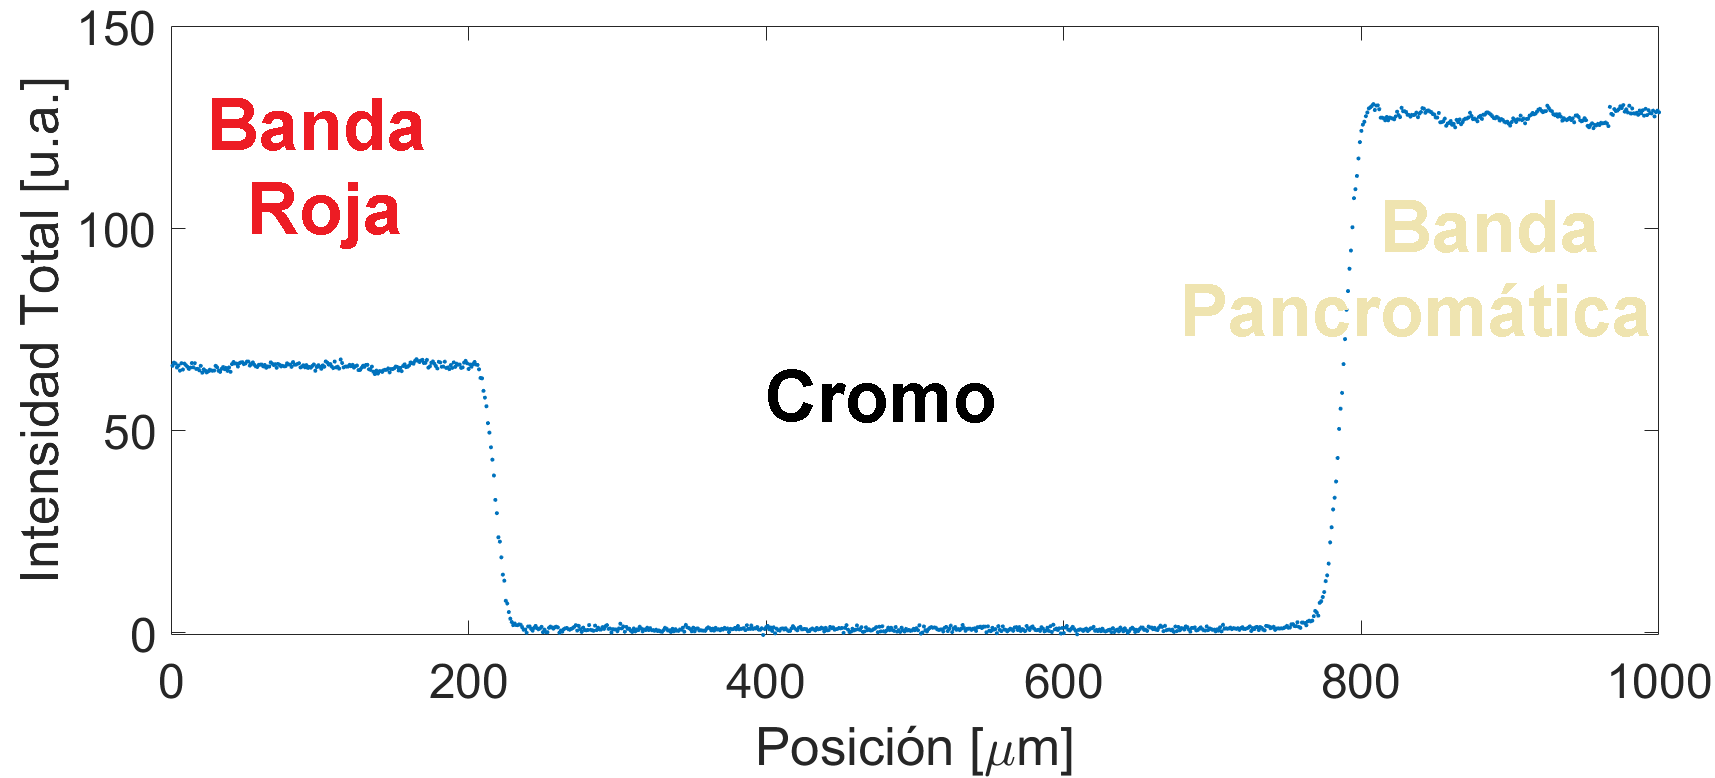
\includegraphics[width=1.0\columnwidth]{Figs/microespectrometro/barridocromocalib.png}
	\caption{Gráfico de la intensidad total detectada en función de la posición medida del filtro en un barrido lineal del cromo que separa las bandas roja de la pancromática.}
	\label{fig:barrcromoo}
\end{figure}

En el gráfico de la Figura \ref{fig:barrcromoo} se muestra la intensidad total detectada, esto es la suma de la intensidad detectada para cada longitud de onda del espectro medido, en función de la posición del filtro. El barrido fue lineal, es decir en una dimensión. Se asignó por \textit{software} a la platina un desplazamiento de 1000 $\mu m$, con un paso de 1 $\mu m$. En cada paso de la platina el microespectrómetro obtuvo una medición del espectro. Los espectros no fueron normalizados con la fuente de luz y es por eso que se puede observar un mayor valor de intensidad total para la banda pancromática que para la banda roja. El valor del cromo que separa la banda roja de la pancromática medido con el \textit{software} Fiji de una imagen completa del filtro adquirida con el microscopio Zeiss fue de $( 516 \pm 10) \mu m$.
Para determinar el valor medido de la longitud del cromo con el microespectrómetro se ajustó cada transición de una banda al cromo con la función error, \textit{erf(x)}, que es la integral del perfil gaussiano del haz de luz en una dimensión. La función utilizada para el ajuste fue, para la transición izquierda y derecha respectivamente:
\begin{equation}
\text{transición\_izquierda} (x,a,b,c) = \frac{a}{2}\hspace{2pt}.\hspace{2pt}erf\left(\sqrt{2}\hspace{1pt}.\hspace{1pt}\frac{(x-b)}{c}\right)
\label{eq:iz}
\end{equation}
\begin{equation}
\text{transición\_derecha} (x,a,b,c) = \frac{a}{2}\hspace{2pt}.\hspace{2pt}\left(1+erf\left(\sqrt{2}\hspace{1pt}.\hspace{1pt}\frac{(x-b)}{c}\right)\right),
\label{eq:der}
 \end{equation} para la transición izquierda [\ref{eq:iz}] y derecha [\ref{eq:der}] respectivamente. Así por ejemplo para el barrido de la Figura \ref{fig:barrcromoo} se ajustaron ambas transiciones como se muestra en las Figuras \ref{fig:ajustess} (a) y (b). En azul se muestra el resultado del ajuste y los puntos rojos fueron datos eliminados de cada ajuste.
\begin{figure}[H]
%\centering
\hfill%
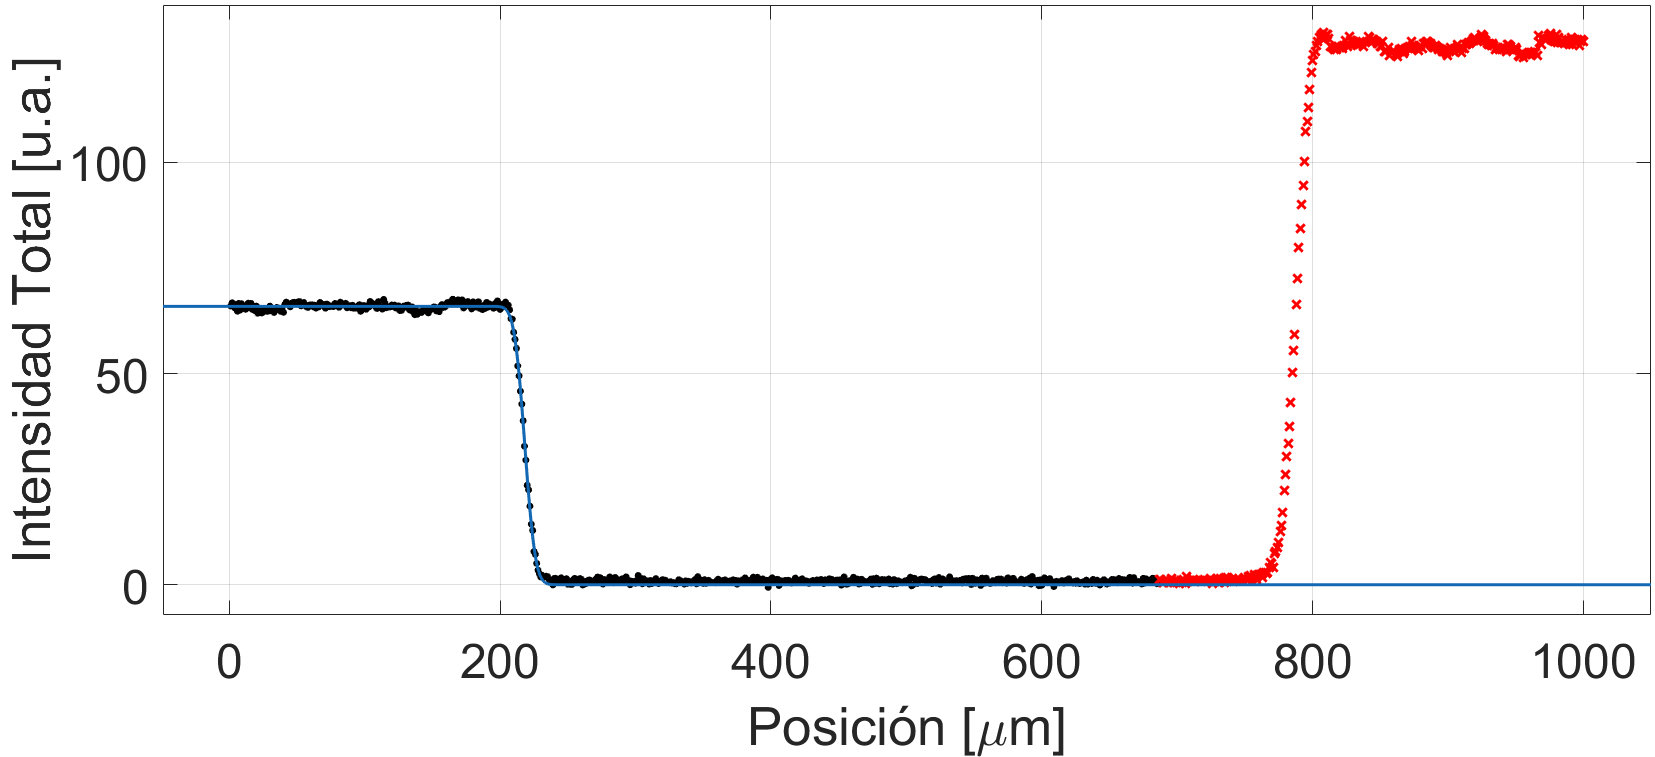
\includegraphics[scale=0.25]{Figs/microespectrometro/ajustebarrladoizq.png}
\hfill%
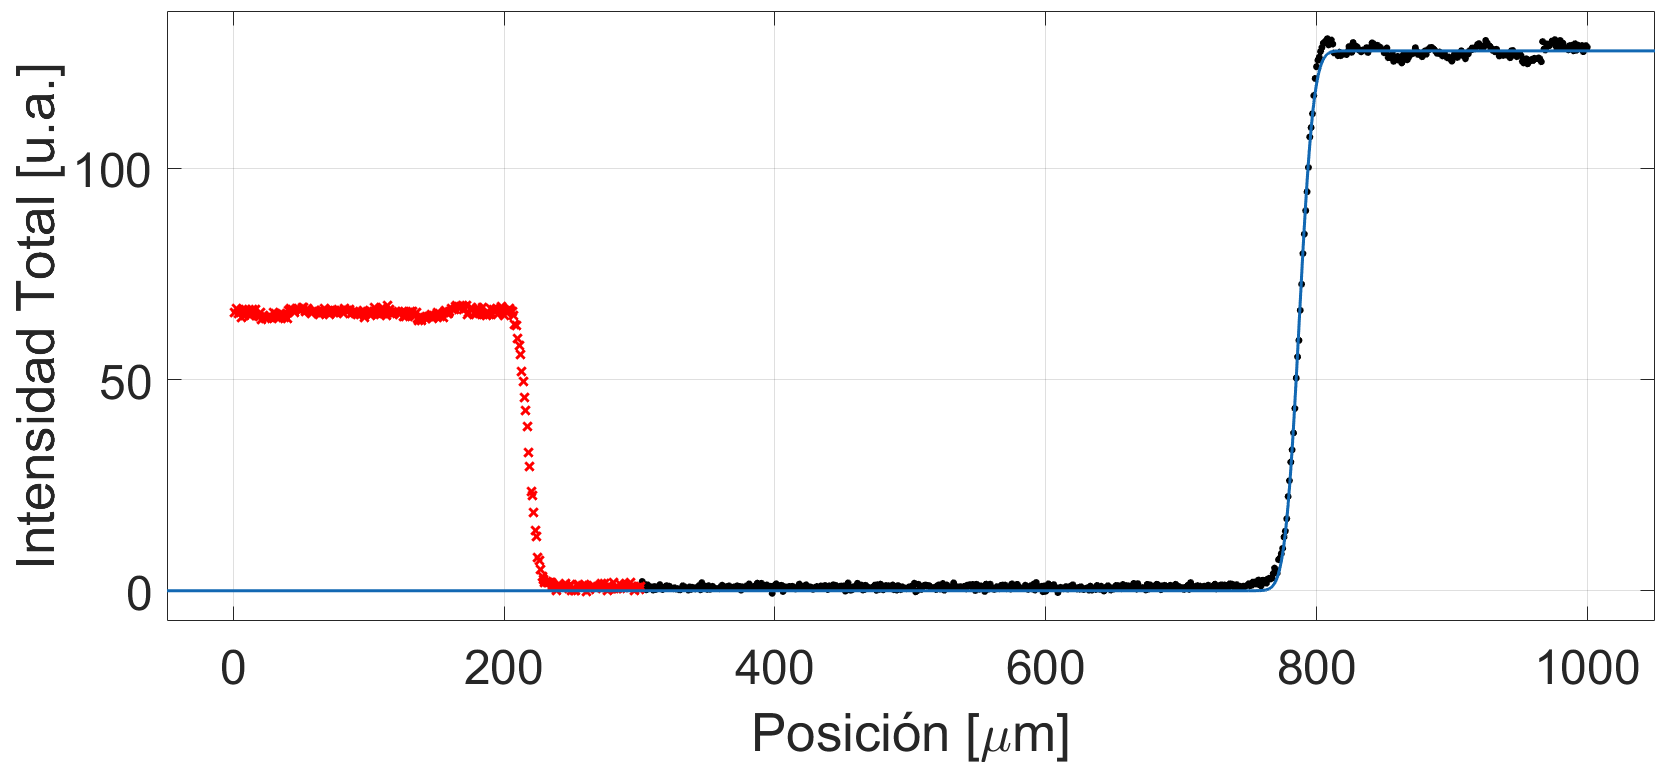
\includegraphics[scale=0.25]{Figs/microespectrometro/ajustebarrladoder.png}
\hfill%
\hfill%
\caption{(a) Ajuste de los datos de la transición de la banda roja al cromo por una función \textit{erf(x)}. (b) Ajuste de los datos de la transición del cromo a la banda pancromática por una función \textit{erf(x)}.}
\label{fig:ajustess}
\end{figure}

A partir de los parámetros del ajuste se determinó la longitud medida del cromo, $l_{cromo}$ de la siguiente manera:
\begin{equation}
l_{cromo} = (b_{der} - c_{der}) - (b_{izq} + c_{izq}),
\end{equation}
donde $b_{izq}, c_{izq}, b_{der} yc_{der}$ son los parámetros del ajuste de la transición entre la banda roja y el cromo (izq) y entre el cromo y la banda pancromática (der). Así, para el barrido que se muestra en la Figura \ref{fig:barrcromoo} se obtuvo una longitud del cromo igual a 540 micrones, con lo cual para esta medición la diferencia entre el valor medido con el microespectrómetro y el valor tomado como referencia medido con el Zeiss, fue del 5\%.

En esta sección se describió la platina desarrollada para poder caracterizar al filtro en cualquier punto del mismo y con la suficiente resolución como para poder muestrear correctamente la resolución óptica del microespectrómetro, que se explica en la Sección \ref{sec:caractequipo}. En el Apéndice \ref{chap:platine} se muestra un resumen de las características principales de la platina desarrollada y las futuras mejoras que serán implementadas.


%%%%%%%%%%%%%%%%%%%%%%%%%%%%%%%%%%%%%%%%%%%%%%%%%%%%%%%%%%%%%%%%%%%%%%%%%%%%%%%%%%%%%%%%%%%%%%%%%%%%%%%%%%%%%%%%%%%%%%%%%%%%%%%%%%%%%%%%%%%%%%%%%%%%%%%%%%%%%%%%%%%%%%%%%%%%%%%%%%%%%%%%%%%%%%%%%%%%%%%%%%%%%%%%%%%%%%%%%%%%

\singlespacing
\subsection{Diseño óptico, montaje y alineación del microespectrómetro}
\label{sec:montalin}
\spacing{1.5}

\hspace{0.5cm}En la Figura \ref{fig:micromfinal} se muestra el montaje y los componentes de la versión actual del microespectrómetro. 
\begin{figure}[H]
	\centering
	\includegraphics[width=1.0\textwidth]{Figs/microespectrometro/microespectrometroo_actual.png}
	\caption{Componentes ópticos y montaje del microespectrómetro.}
	\label{fig:micromfinal}
\end{figure}
El diagrama del camino óptico del microespectrómetro se muestra en la Figura \ref{fig:diagcaminoopt}. La luz que sale divergente de la fibra óptica (Ver Figura \ref{fig:montttluz}) incide perpendicularmente sobre el filtro. La luz transmitida por el filtro es recolectada por un objetivo de microscopio \href{https://www.edmundoptics.com/p/10x-mitutoyo-plan-apo-infinity-corrected-long-wd-objective/6623/}{Mitutoyo} corregido al infinito, de distancia de trabajo larga (34 mm), magnificación 10X y una apertura numérica igual a 0.28. La luz que sale corregida al infinito del objetivo es enfocada con una lente biconvexa de distancia focal igual a 200 mm de forma simultánea a la fibra del espectrómetro y a un sensor CMOS de una cámara \href{https://www.microsoft.com/accessories/es-xl/d/lifecam-hd-3000}{Lifecam HD 3000}, por medio de un \textit{beamsplitter} 10:90 (R:T) \href{https://www.thorlabs.com/thorproduct.cfm?partnumber=BSN10R}{BSN10R}. El \textit{beamsplitter} refleja un 10\% de la luz a la cámara y transmite el 90\% a la fibra óptica acoplada al espectrómetro. 
\begin{figure}[H]
	\centering
	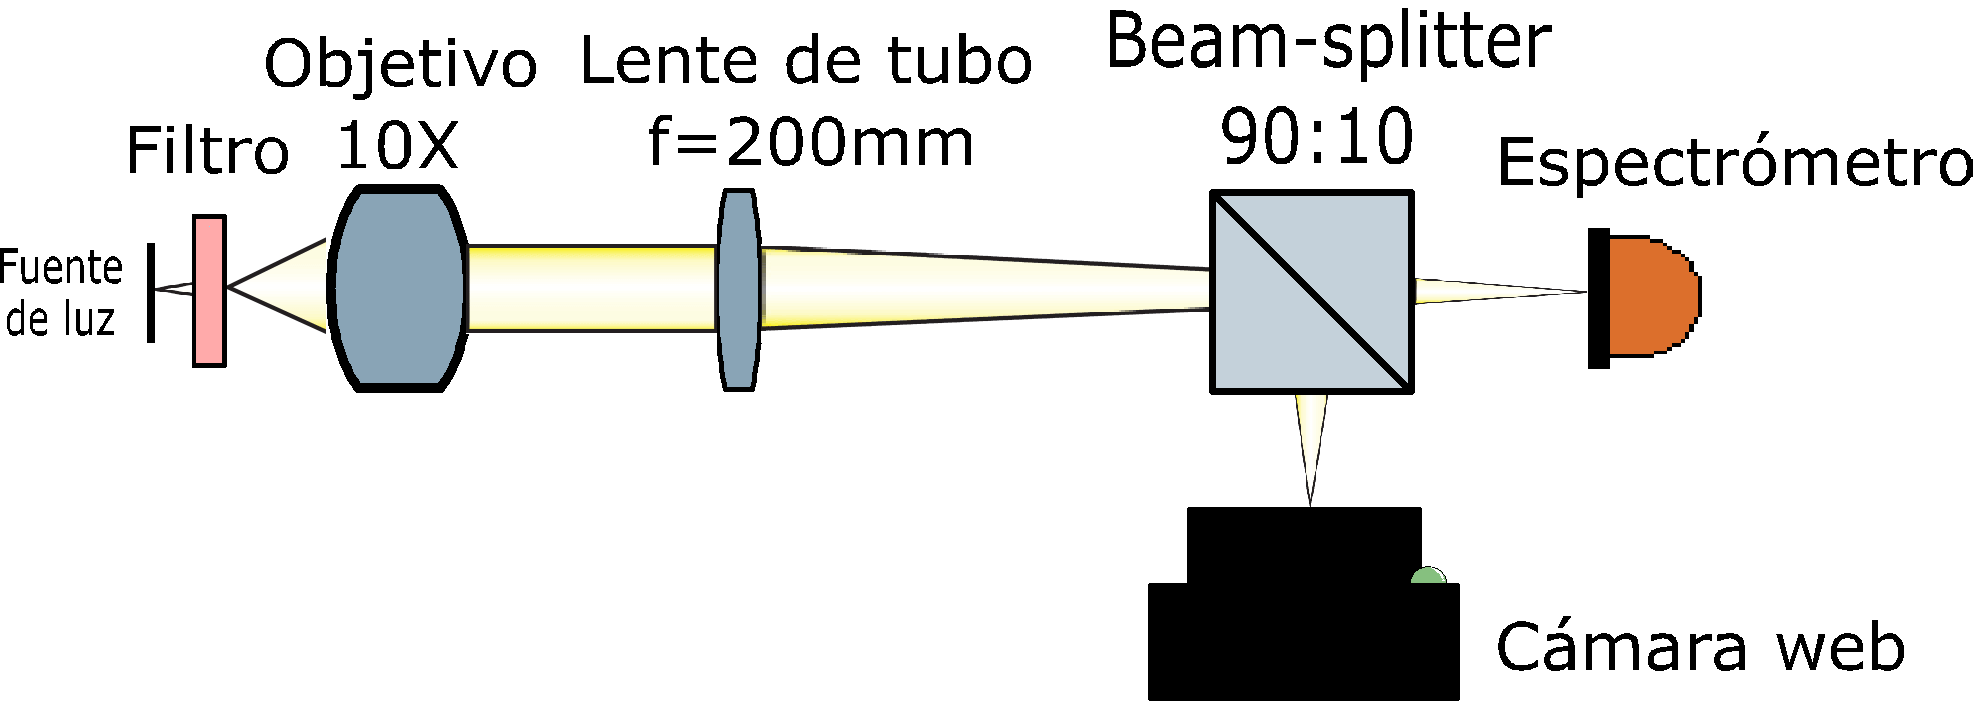
\includegraphics[width=1.0\textwidth]{Figs/microespectrometro/diagopticosetup.png}
	\caption{Diagrama del camino óptico del microespectrómetro.}
	\label{fig:diagcaminoopt}
\end{figure}

El objetivo fue montado sobre un componente optomecánico \href{https://www.thorlabs.com/thorProduct.cfm?partNumber=SM1Z\#ad-image-0}{SM1Z} de Thorlabs que permitió modificar la distancia entre el objetivo y el filtro para poner en foco al microespectrómetro (Ver Sección \ref{sec:focoresol}). El SM1Z tiene una longitud de recorrido de 2 mm, paso de 1 $\mu m$ y por cada revolución se tiene un desplazamiento lineal de 50 $\mu m$.  La lente de tubo (en inglés, \textit{tube lens}) fue montada sobre un \href{https://www.thorlabs.com/thorproduct.cfm?partnumber=SM1V15}{SM1V15} que permitió modificar la distancia entre la lente de tubo y la fibra del espectrómetro para su alineación. El SM1V15 fue montado sobre un \textit{cage} CP33. El beamsplitter de forma rectangular fue sujetado por un adaptador \href{https://www.thorlabs.com/thorproduct.cfm?partnumber=FFM1\#ad-image-0}{FFM1} y éste fue asegurado con dos tornillos sobre la tapa del cubo \href{https://www.thorlabs.com/thorproduct.cfm?partnumber=C6W}{C6W}. La fibra óptica del espectrómetro se conectó al \textit{cage} \href{https://www.thorlabs.com/thorproduct.cfm?partnumber=CXY1\#ad-image-0}{CXY1} que tiene una longitud de recorrido en \textit{x} e \textit{y} de 1 mm para ajustar su posición. La cámara fue colocada sobre un \textit{cage} impreso en una impresora 3D [\href{https://github.com/jrr1984/open_frame_XYStage/blob/master/3dprintedparts/STLs/CAGE\_1pulgada.STL}{\faCubes$_{4}$}]. Todo el sistema fue montado con barras de 6 mm de diámetro de Thorlabs.

Para alinear la fuente de luz con el objetivo, se retiró el filtro del medio del sistema de iluminación y de detección con la platina (subiéndolo hacia arriba, no hizo falta desmontarlo) y se alineó el \textit{cage} de la fibra óptica de la fuente de luz con el SM1Z del objetivo. De esta manera se alineó el plano perpendicular al eje óptico (eje $\textit{z}$) contenido por los ejes $\textit{x} e \textit{y}$ (ver Figura \ref{fig:plato0}) entre la fuente de luz y el microespectrómetro. Esta alineación fue realizada para maximizar la intensidad de la luz detectada.

La alineación de la lente de tubo y del objetivo fueron realizadas de forma previa al montaje final del equipo. Para alinear la lente de tubo (Ver Figura \ref{fig:ali} (a)), en primer lugar se colimó la fuente de luz con una lente plano convexa \href{https://www.thorlabs.com/thorproduct.cfm?partnumber=LA1951}{LA1951} de distancia focal igual a 1 pulgada y diámetro de 1 pulgada (\textit{f-number} igual a 1). La luz colimada fue enfocada por la lente de tubo a la fibra del espectrómetro. Se refinó la distancia entre la lente de tubo y la fibra del espectrómetro a partir del ajuste manual del SM1V15 observando la intensidad total detectada con el espectrómetro. Se fijó dicha distancia en el máximo de intensidad detectado, asegurando el anillo del SM1V15 al \textit{cage} sobre el que estaba montado.

Respecto de la alineación del objetivo (Ver Figura \ref{fig:ali} (b)), se hizo foco en la superficie exterior del filtro más cercana al mismo. Para ello se utilizó la fuente de luz colimada y un beamsplitter 50:50 para redirigir la luz hacia el objetivo que a su vez enfocó la luz en la superficie exterior del filtro. A partir de la reflexión en el filtro que se transmite por el objetivo y luego por el beamsplitter, se observó la luz colimada con una pantalla situada en `el infinito'.  Se refinó el grado de colimación de la luz, variando la distancia entre el objetivo y el filtro con la perilla manual de paso micrométrico del SM1Z. De esta forma, se aseguró que el objetivo está recolectando la luz del plano focal asociado a la superficie exterior del filtro más cercana al objetivo que es la que se quiere observar. 
\begin{figure}[H]
%\centering
\hfill%
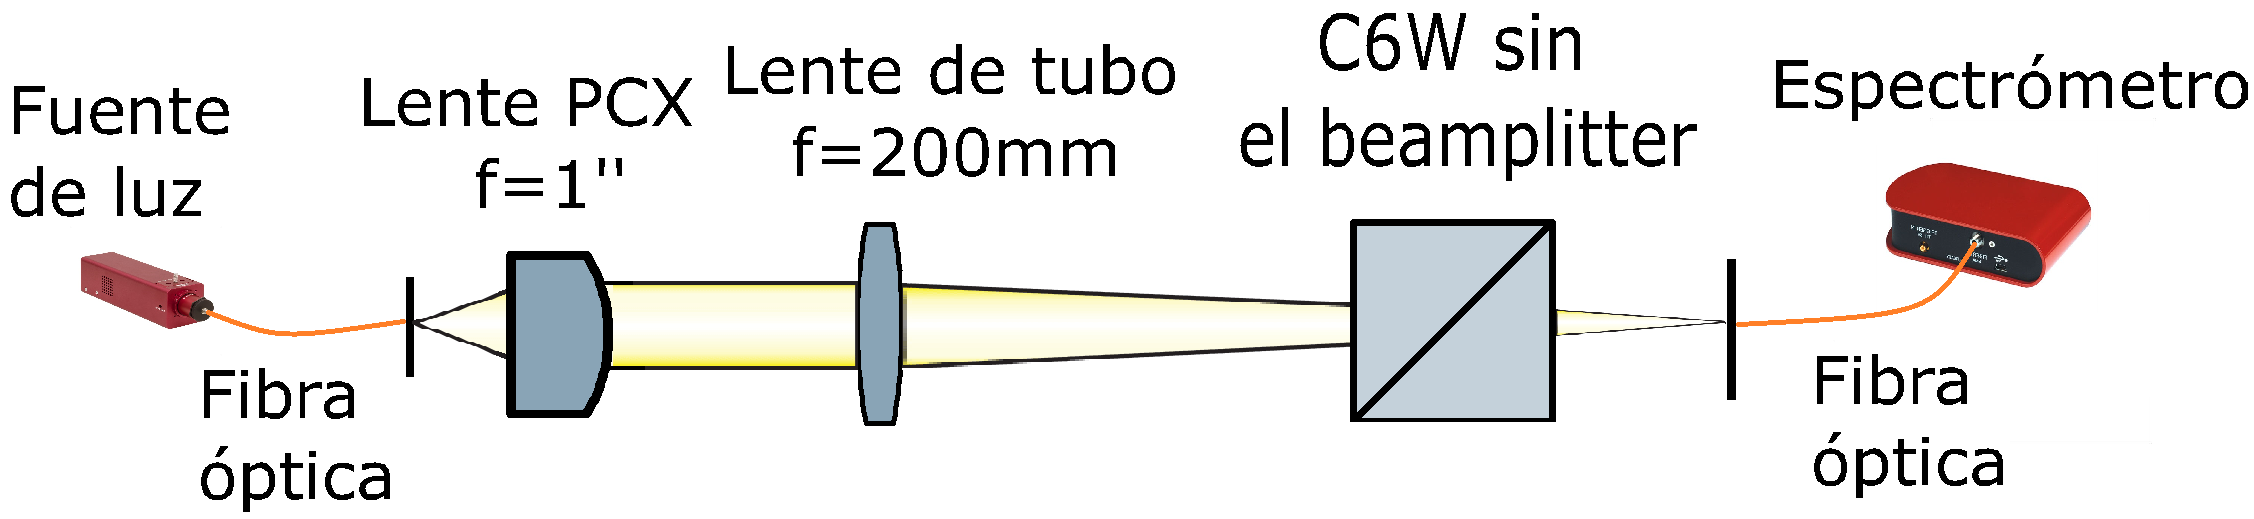
\includegraphics[width=1.0\textwidth]{Figs/microespectrometro/diagoptico_alinetubel.png}
\hfill%
\vspace{0.1cm}
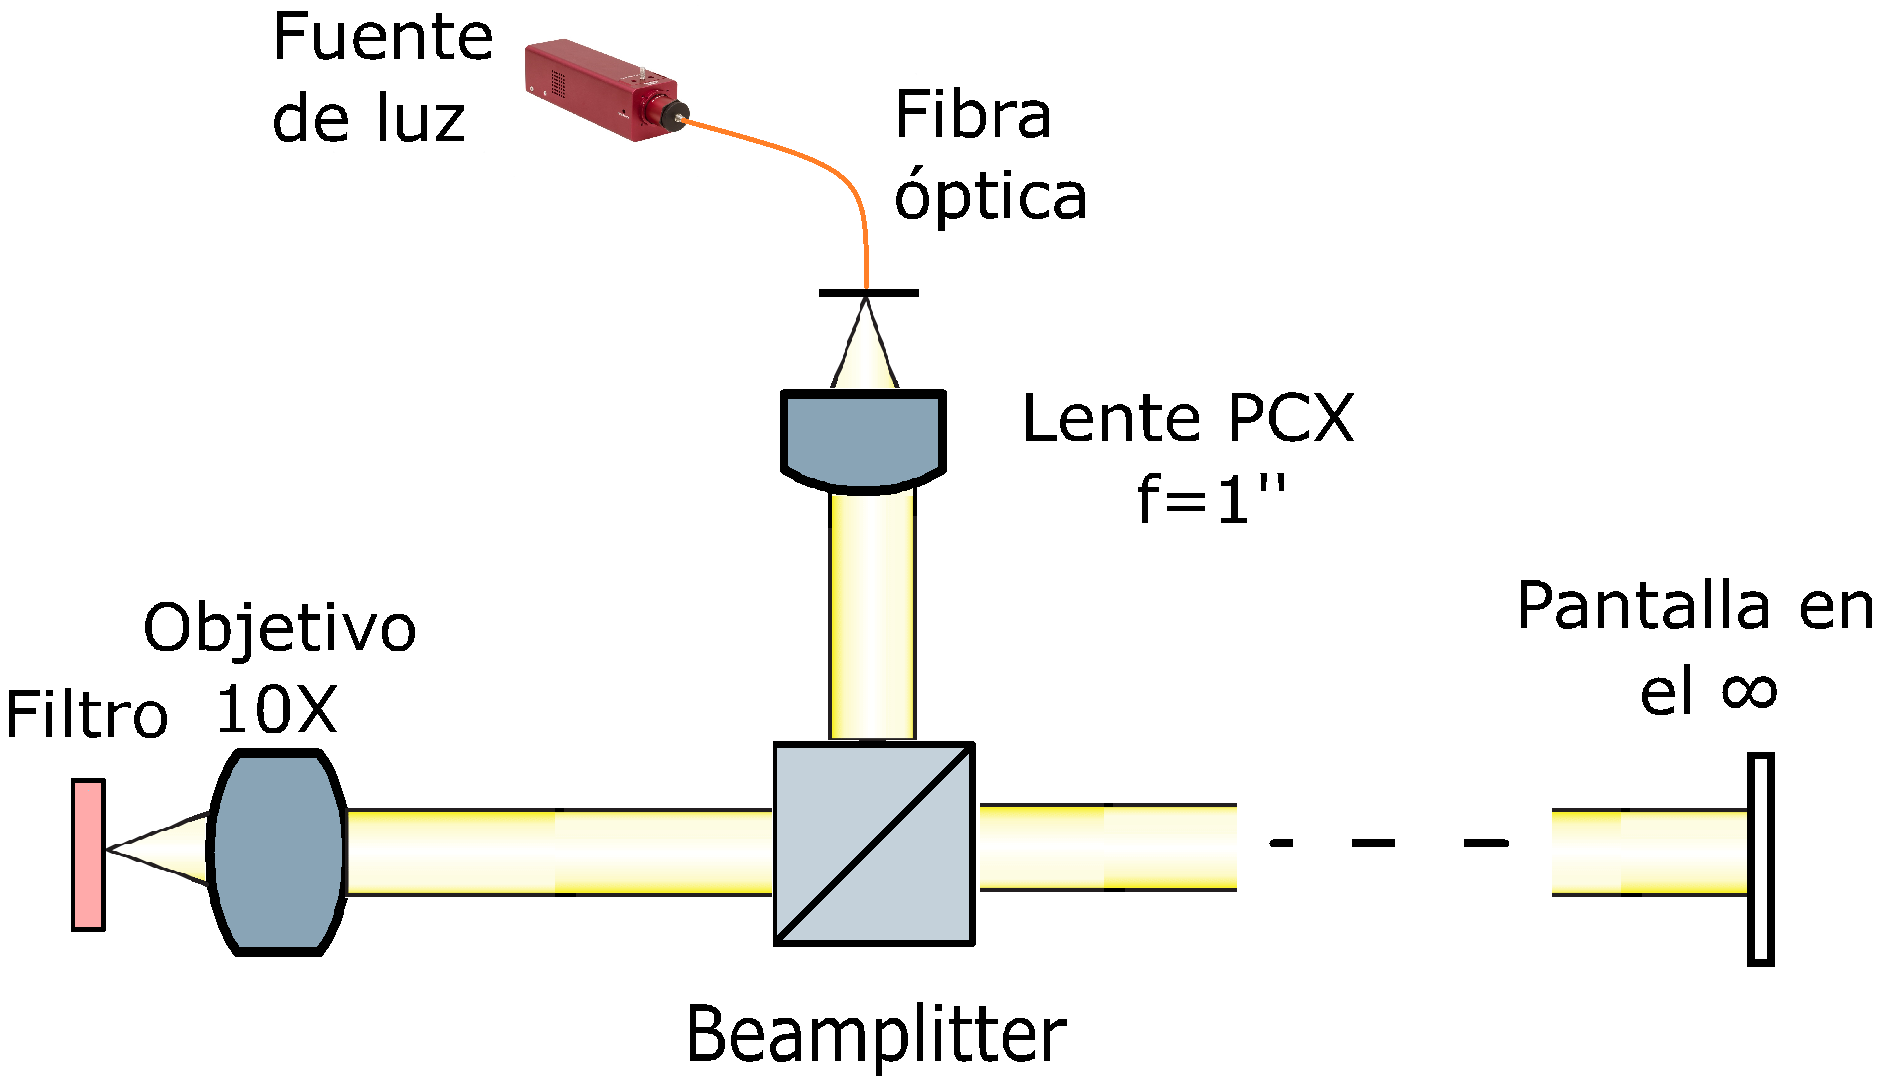
\includegraphics[width=1.0\textwidth]{Figs/microespectrometro/diagoptico_alineobjet.png}
\hfill%
\hfill%
\caption{(a) Diagrama óptico de la alineación de la lente de tubo del microespectrómetro. (b) Diagrama óptico de la alineación del objetivo del microespectrómetro.}
\label{fig:ali}
\end{figure}

Luego de enfocar el objetivo, se incorporó la lente de tubo alineada, uniendo ambas partes con las barras de 6 mm en el sistema de \textit{cages}. Ahora bien, como el filtro al desplazarse con la platina puede salirse de foco dado que el desplazamiento no es perfectamente perpendicular al eje óptico, se determinó un método para poner en foco el microespectrómetro con el equipo montado completamente a partir de la medición de la resolución espacial como se explica en la Sección \ref{sec:focoresol}.

%%%%%%%%%%%%%%%%%%%%%%%%%%%%%%%%%%%%%%%%%%%%%%%%%%%%%%%%%%%%%%%%%%%%%%%%%%%%%%%%%%%%%%%%%%%%%%%%%%%%%%%%%%%%%%
%%%%%%%%%%%%%%%%%%%%%%%%%%%%%%%%%%%%%%%%%%%%%%%%%%%%%%%%%%%%%%%%%%%%%%%%%%%%%%%%%%%%%%%%%%%%%%%%%%%%%%%%%%%%%%


\singlespacing
\subsection{Integración de una cámara. Adquisición simultánea de imágenes y de espectros de transmisión mediante una interfaz gráfica \href{https://github.com/jrr1984/defectsGUI}{\faGithub$_{3.2.4}$}}
\label{sec:camwebgui}
\spacing{1.5}

\hspace{0.5cm}Previo a la integración de la cámara, la única información que se tenía de la región a medir del filtro consistía de los espectros de transmisión medidos, es decir se tenían los gráficos de la intensidad detectada en función de la longitud de onda de cada medición. Así por ejemplo, en la Figura \ref{fig:muchossi} se muestra un barrido lineal de  800 $\mu m$, con un paso de 1 $\mu m$, elegidos en el \textit{software} de adquisición, desde la banda pancromática hasta el cromo. 

 \begin{figure}[H]
	\centering
	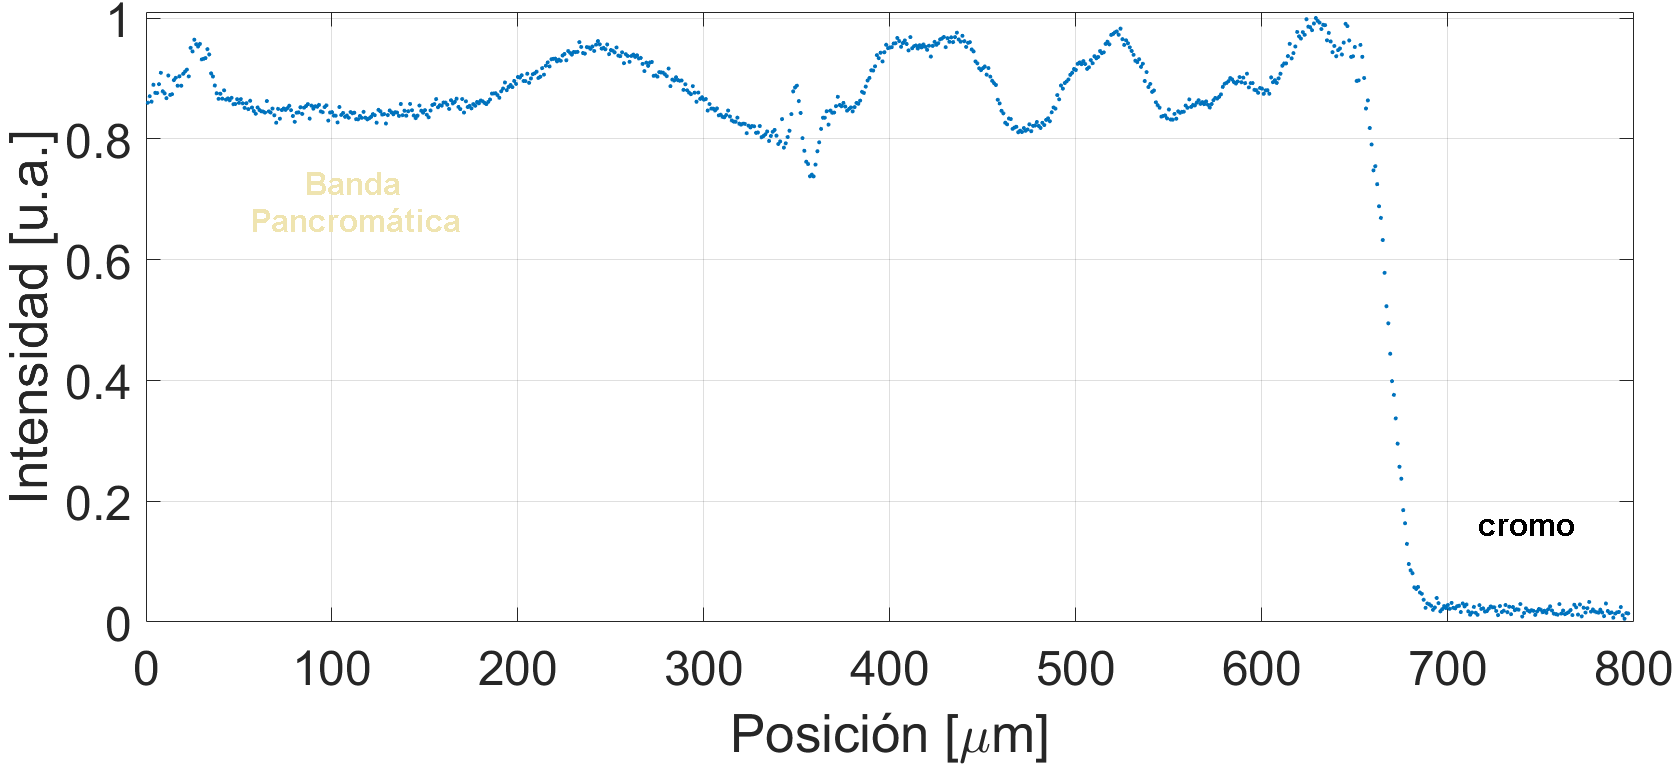
\includegraphics[width=1.0\textwidth]{Figs/microespectrometro/defectosmuchossinvis.png}
	\caption{Barrido lineal realizado de 150 $\mu m$, desde la banda azul hacia el cromo atravesando el defecto que se señala en la imagen.}
	\label{fig:muchossi}
\end{figure}

El gráfico de la Figura \ref{fig:muchossi} consiste de la suma de las intensidades detectadas para cada longitud de cada medición normalizadas con su máximo valor, en función de la posición del filtro. En la región medida del filtro comprendida por la banda pancromática que se extiende desde la posición inicial hasta aproximadamente los 645 $\mu m$, se puede observar que la intensidad transmitida por dicha banda no es uniforme como debería ser. Es decir, se podría tomar como hipótesis que cada uno de los `valles' detectados se corresponde con un defecto pero al no tener un \textit{feedback} visual, resulta imposible de corroborar siendo que no se conoce de antemano la firma espectral de los distintos defectos. Más aún, esto último era lo que se quería determinar con el equipo desarrollado.  

Esto motivó la integración de la cámara en el equipo. Con el objetivo de poder visualizar en vivo y de forma simultánea una imagen de la región del filtro que se estaba midiendo y el espectro de transmisión se desarrolló una interfaz gráfica que fue organizada como se muestra en el diagrama de cajas de la Figura \ref{fig:diagcajas}.

\begin{figure}[H]
	\centering
	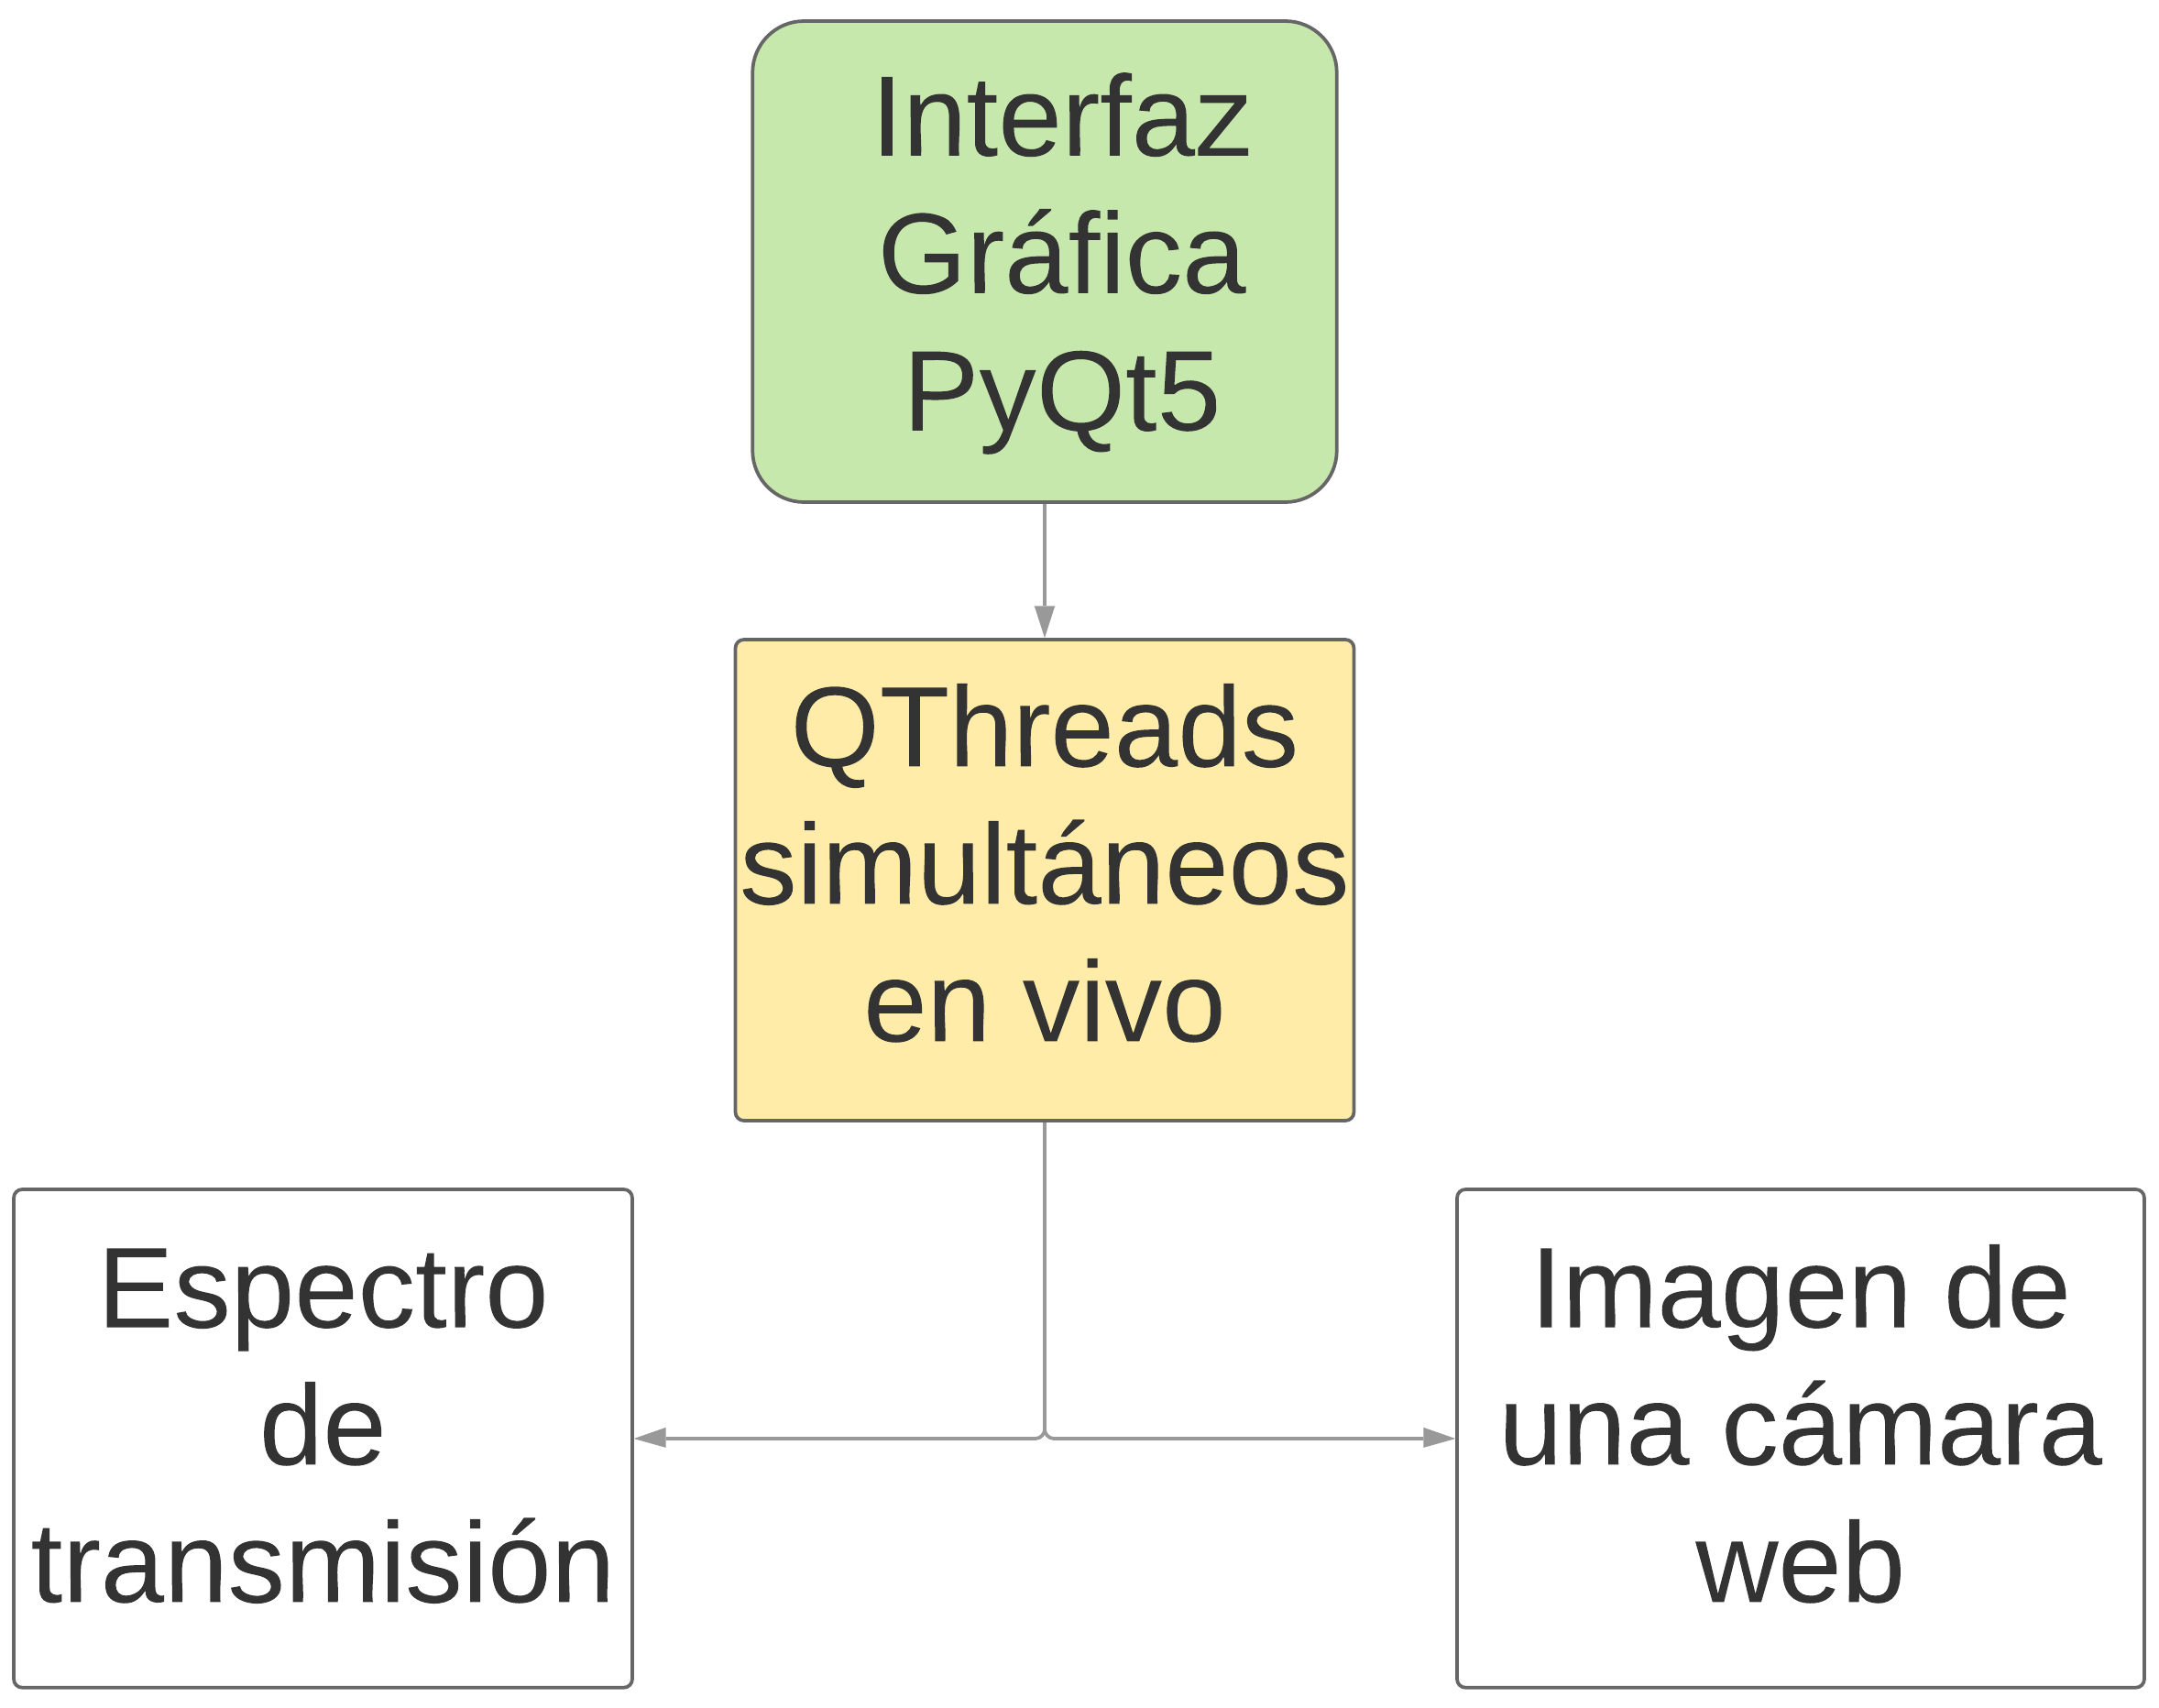
\includegraphics[scale=0.5]{Figs/microespectrometro/interfazespcam.png}
	\caption{Diagrama de cajas de la interfaz gráfica desarrollada para visualizar en vivo simultáneamente el espectro de transmisión y la imagen de una cámara.}
	\label{fig:diagcajas}
\end{figure}

Se desarrollaron dos clases en el lenguaje de programación \textit{python} para controlar en vivo la cámara [\href{https://github.com/jrr1984/defectsGUI/blob/master/views.py}{\faGithub$_{3.2.4.2}$}] y el espectrómetro [\href{https://github.com/jrr1984/defectsGUI/blob/master/Spectrometer.py}{\faGithub$_{3.2.4.3}$}]. Luego con la librería \href{https://pypi.org/project/PyQt5/}{PyQt5} se desarrolló una interfaz gráfica que fue implementada por medio de dos \textit{QThreads} que son dos objetos que corrieron de forma paralela e independiente en el mismo proceso. La interfaz gráfica permitió poder visualizar tanto la imagen como el espectro de la posición del filtro que estaba siendo iluminada y al mismo al recorrer el fltro desplazándolo con el \textit{joystick} de la platina por las regiones de interés. En la Figura \ref{fig:inaaa} se muestra la interfaz gráfica desarrollada (\textit{script} para correr la GUI: \href{https://github.com/jrr1984/defectsGUI/blob/master/start.py}{\faGithub$_{3.2.4.4}$}).

\begin{figure}[H]
	\centering
	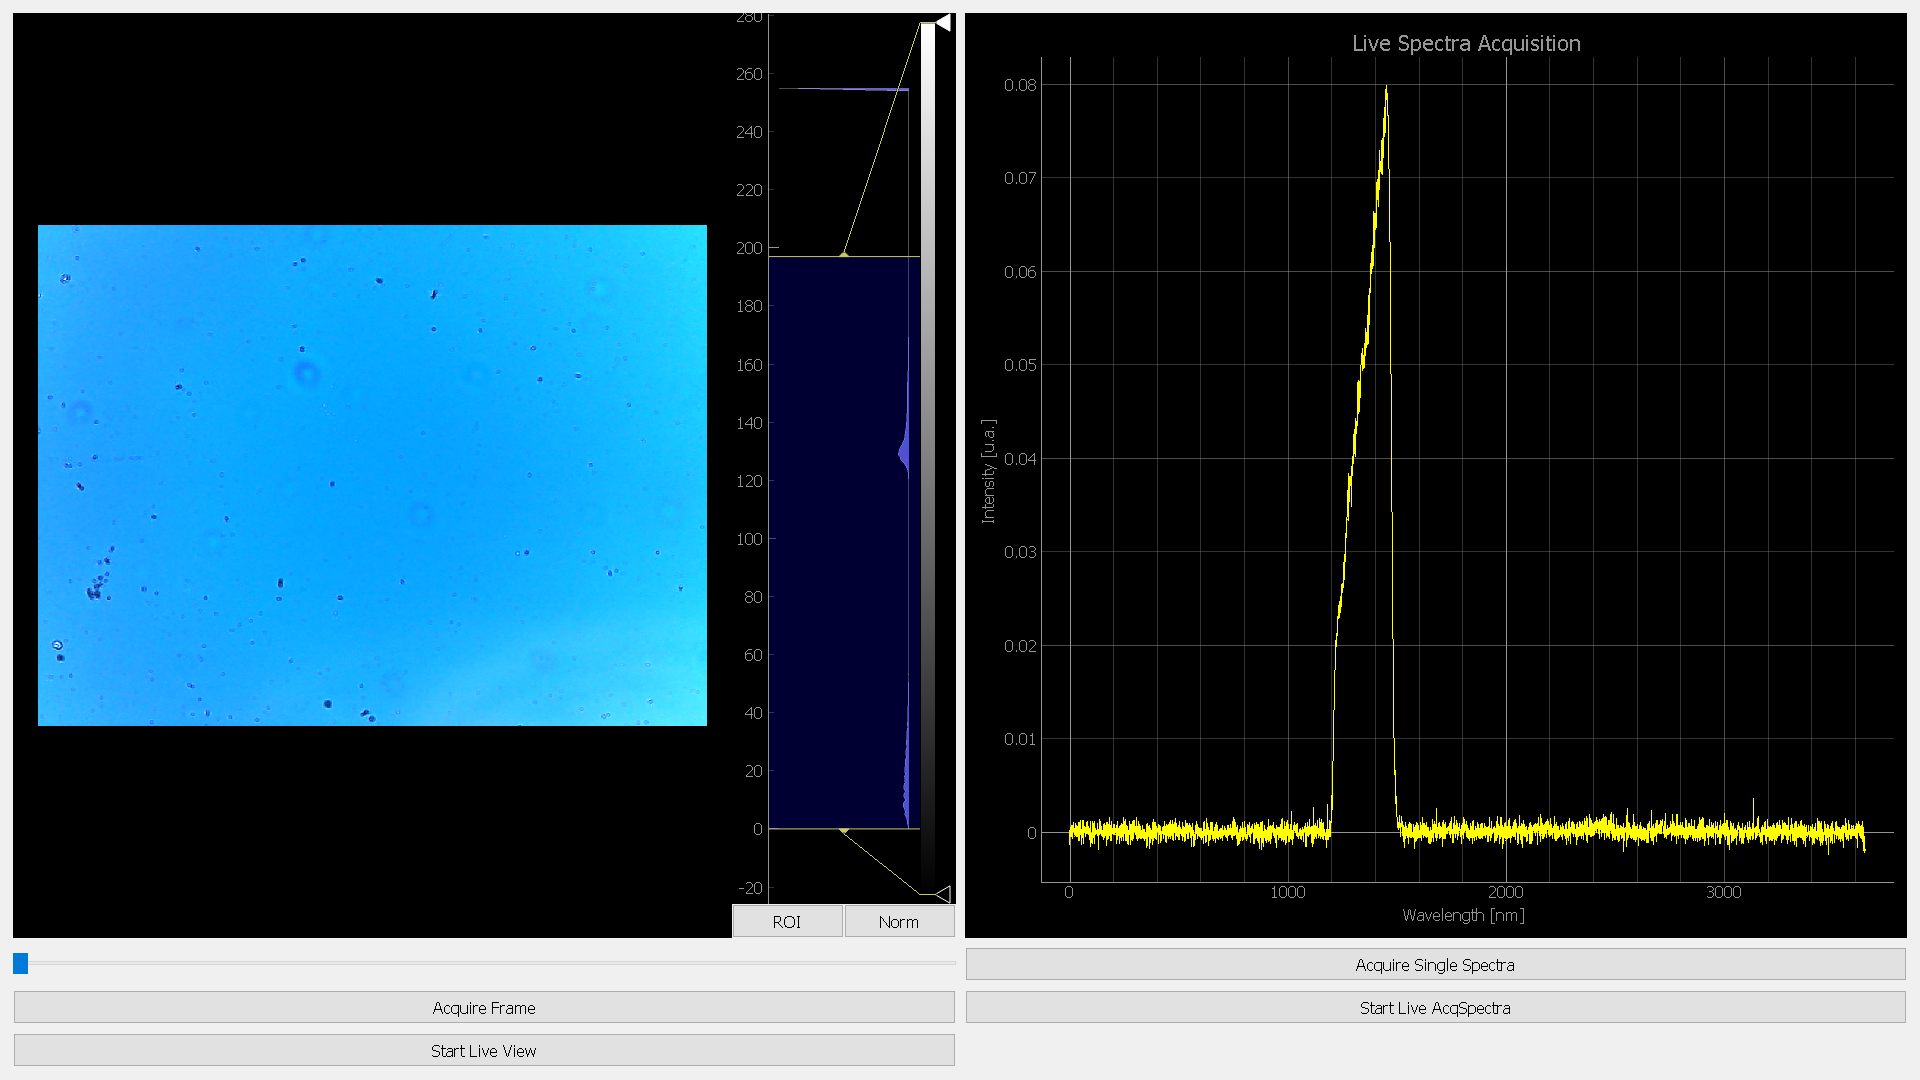
\includegraphics[width=1.0\textwidth]{Figs/microespectrometro/medicionbandacelesteGUI.png}
	\caption{Interfaz gráfica desarrollada para visualizar en vivo simultáneamente el espectro de transmisión y la imagen de una cámara [\href{https://github.com/jrr1984/defectsGUI/blob/master/start.py}{\faGithub$_{3.2.4.4}$}].}
	\label{fig:inaaa}
\end{figure}

 
%%%%%%%%%%%%%%%%%%%%%%%%%%%%%%%%%%%%%%%%%%%%%%%%%%%%%%%%%%%%%%%%%%%%%%%%%%%%%%%%%%%%%%%%%%%%%%%%%%%%%%%%%%%%%%
%%%%%%%%%%%%%%%%%%%%%%%%%%%%%%%%%%%%%%%%%%%%%%%%%%%%%%%%%%%%%%%%%%%%%%%%%%%%%%%%%%%%%%%%%%%%%%%%%%%%%%%%%%%%%%

\singlespacing
\subsection{\textit{Software} automatizado de adquisición de los espectros de transmisión \href{https://github.com/jrr1984/open\_frame\_XYStage/blob/master/main.py}{\faGithub$_{3.2.5}$}}
\label{sec:softadq}
\spacing{1.5}

 \hspace{0.5cm}Para realizar las mediciones de forma automatizada de los espectros de transmisión y de forma sincronizada con los desplazamientos de los motores de la platina se desarrolló un \textit{software} de control cuya implementación fue organizada como se muestra en el diagrama de flujo de la Figura \ref{fig:ddinaaa}.

En el \textit{main} [\href{https://github.com/jrr1984/open_frame_XYStage/blob/master/main.py}{\faGithub$_{3.2.5}$}] principal del \textit{software} se eligieron los parámetros del barrido a realizar sobre la región del filtro que se queria medir su espectro de transmisión. Se eligieron las dimensiones del barrido, es decir la longitud a recorrer por cada eje de la platina y el paso a realizar que determina el número de mediciones del barrido completo. También entre los parámetros del barrido se eligieron el tiempo de integración de la luz del espectrómetro y el número de espectros que se adquiere por medición para tomar el valor medio de los mismos.
 
 \begin{figure}[H]
	\centering
	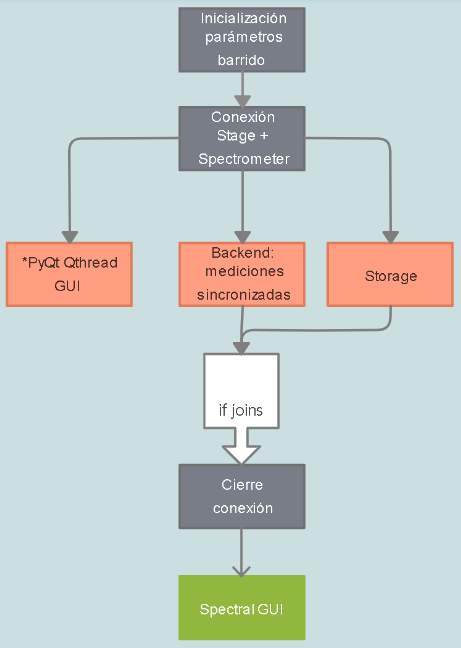
\includegraphics[width=1.0\textwidth]{Figs/microespectrometro/flowdiagprot0.png}
	\caption{Diagrama de flujo del software automatizado de adquisición de los espectros de transmisión.}
	\label{fig:ddinaaa}
\end{figure}



Las mediciones de los espectros de transmisión medidos de cada posición asignada a la platina, denominado el \textit{thread} del \textit{backend} del proceso, se realiza de forma paralela e independiente del guardado de las mediciones en disco que consiste de otro \textit{thread} del mismo proceso. Un \textit{thread} consiste de un conjunto de ejecuciones que son parte de un proceso computacional. Con la librería \textit{mutltithreading} se implementaron estos dos \textit{threads} de forma tal que si la medición era o tenía que ser interrumpida por algún motivo, el guardado de los datos se realizaba en cualquier caso, lo que resultó importante para las mediciones de larga duración. Una vez finalizado el barrido completo de las mediciones, en la interfaz de \textit{cutelog} se podía observar si la medición había concluido de forma correcta, si se habían guardado las mediciones, la duración total, así como la verificación de la desconexión de la platina y del espectrómetro.

Por último, el resultado de las mediciones pudo ser visualizado en la interfaz gráfica interactiva realizada (Ver Figura \ref{fig:GUI00}) para poder realizar mapas multiespectrales de los barridos así como mapas de transmisión.
En esta sección se describió el diseño y construcción del microespectrómetro y de la platina así como todo el desarrollo del \textit{software} necesario para la adquisición automatizada de mediciones y para la visualización en vivo de las mismas. A continuación se describe una caracterización del microespectrómetro a partir de la determinación experimental de la resolución óptica y del proceso de la puesta en foco del equipo para su aplicación, compuesto por el microespectrómetro y por la cámara. 
 

%%%%%%%%%%%%%%%%%%%%%%%%%%%%%%%%%%%%%%%%%%%%%%%%%%%%%%%%%%%%%%%%%%%%%%%%%%%%%%%%%%%%%%%%%%%%%%%%%%%%%%%%%%%%%%
\singlespacing
\section{Caracterización del microespectrómetro}
\label{sec:caractequipo}
\spacing{1.5}

\hspace{0.5cm}La puesta en foco de la cámara de un microscopio digital comercial suele ser inmediata a partir de la visualización de la imagen a adquirir en vivo con un \textit{software} dedicado, buscando el máximo del contraste visual y la nitidez de la imagen. Ahora bien con un equipo como el desarrollado aquí que contempla la adquisición simultánea de un espectro de transmisión y de una imagen digital, el proceso de la puesta en foco tuvo que ser desarrollado. En la Sección \ref{sec:montalin} se describió la puesta en foco preliminar del objetivo. Al montar el microespectrómetro completo, es decir al unir el montaje de la lente de tubo con el objetivo, se tuvo que refinar el foco del objetivo. En la Figura \ref{fig:diagpuestfoc} se muestra el diagrama de flujo del proceso de la puesta en foco de la región del filtro a medir con el equipo.

\begin{figure}[H]
	\centering
	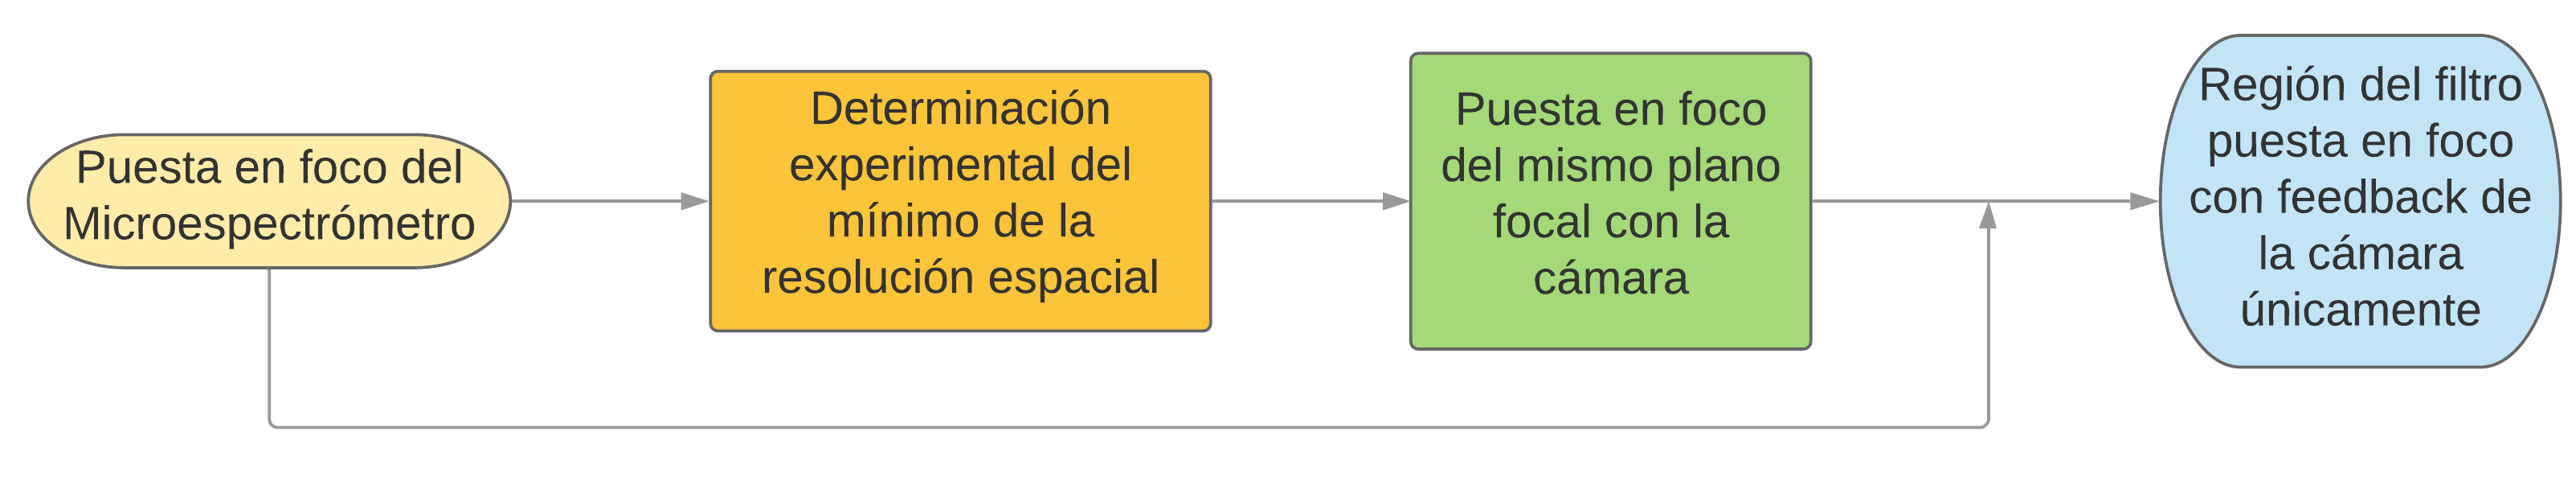
\includegraphics[width=1.0\textwidth]{Figs/microespectrometro/diagramfoco.png}
	\caption{Diagrama de flujo del proceso de la puesta en foco de la región del filtro a medir con el equipo.}
	\label{fig:diagpuestfoc}
\end{figure}

%%%%%%%%%%%%%%%%%%%%%%%%%%%%%%%%%%%%%%%%%%%%%%%%%%%%%%%%%%%%%%%%%%%%%%%%%%%%%%%%%%%%%%%%%%%%%%%%%%%%%%%%%%%%%%



\singlespacing
\subsection{Resolución espacial y foco del microespectrómetro}
\label{sec:focoresol}
\spacing{1.5}

\hspace{0.5cm}En primer lugar se puso en foco el microespectrómetro sobre alguna región de la superficie externa del filtro más cercana al objetivo. Para poner en foco el microespectrómetro se determinó el mínimo de la resolución espacial. En particular, en este trabajo se hace referencia a la resolución espacial lateral, en el plano $\textit{x},\textit{y}$, perpendicular al eje óptico (axial, $\textit{z}$). A continuación se explica la estimación teórica de la resolución espacial, el proceso de medición de la misma y como se determinó el foco del microespectrómetro.

Si bien la resolución espacial medida podría depender de la banda en la cual se realicen las mediciones, debido a la variación de la longitud de onda, el proceso general de la puesta en foco del equipo es independiente de la misma. Para medir la resolución espacial se realizó un barrido de la transición entre el cromo y una banda, en una cierta región del filtro. Esto es, se adquirió el espectro de transmisión para cada desplazamiento del filtro realizado con la platina, de un paso igual a 1 $\mu m$ y con un recorrido tal que la transición entre la banda y el cromo sea realizado de forma completa, ambos elegidos con el \textit{software} de adquisición. Para cada medición del espectro se sumó la intensidad detectada para cada longitud de onda y se normalizó a su vez cada valor por el máximo valor de la intensidad de la suma, en adelante la intensidad total. De esta manera la intensidad total normalizada expresa qué fracción de la luz se transmite, siendo igual a 1 para el caso en que se mida el espectro sobre la banda e igual a aproximadamente 0 para el caso en que se mida el espectro sobre el cromo. En la transición de los valores de intensidad desde la banda hasta el cromo, se pudo determinar la resolución espacial del microespectrómetro a partir del ajuste con la función $\textit{erf(x)}$, que es la integral del perfil gaussiano del haz de luz en una dimensión \cite{LASCH}. 

Se graficó la intensidad total normalizada en función de la posición del filtro. En las Figuras \ref{fig:bgresol} (a) y (b) se muestran dos barridos distintos entre la banda pancromática y el cromo con una resolución espacial de $(292 \pm 12)~ \mu m$, donde dicha resolución fue la peor medida, de un valor más de 29 veces más grande al valor esperado teóricamente, y con una resolución espacial de $(11 \pm 1)~ \mu m$ respectivamente, donde este último valor se solapa con el valor esperado teóricamente de 10 $\mu m$ como se explica a continuación.

\begin{figure}[H]
%\centering
\hfill%
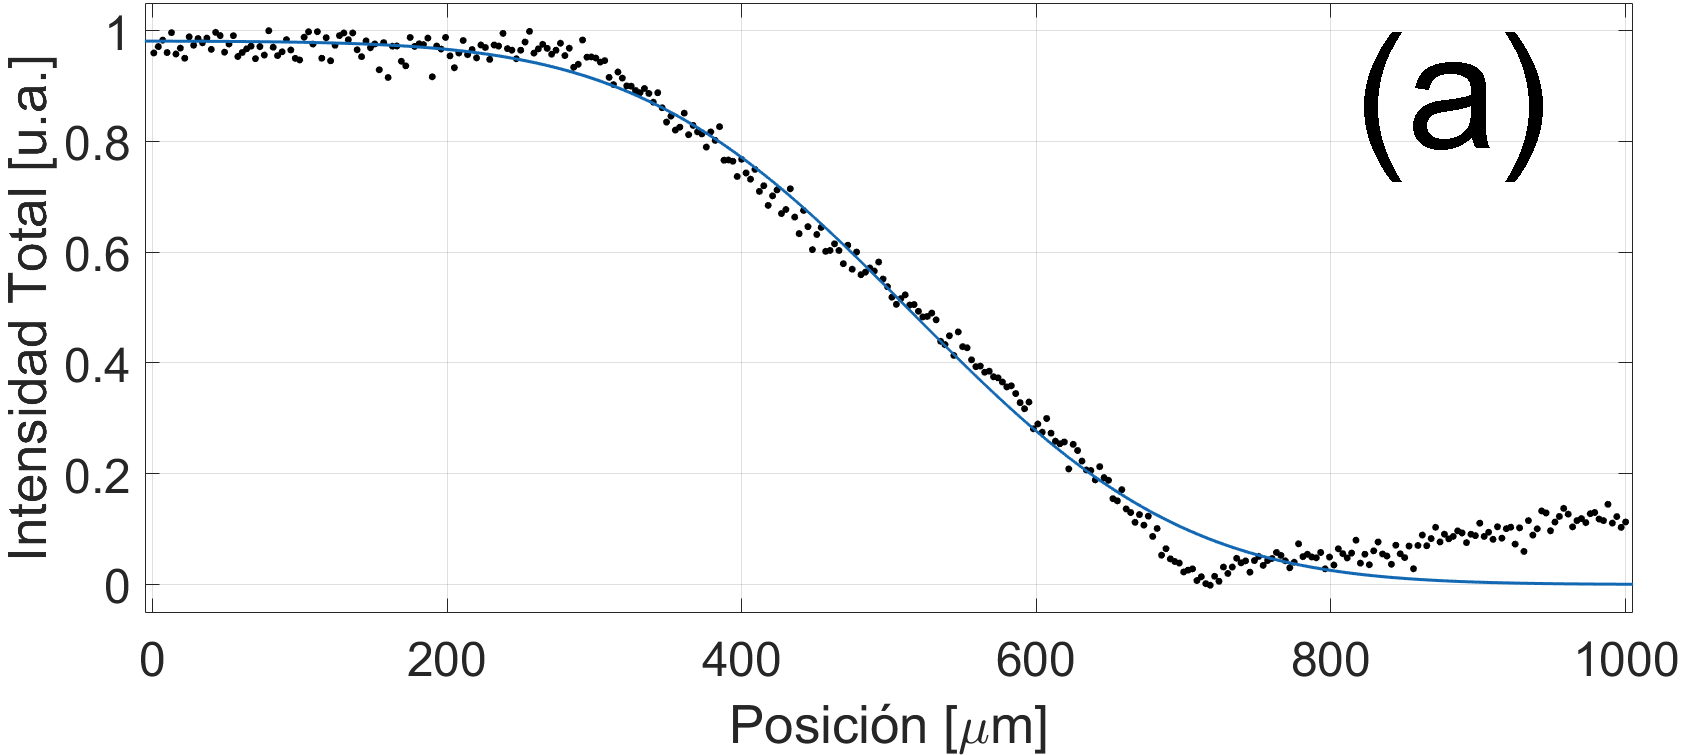
\includegraphics[scale=0.25]{Figs/microespectrometro/badresol.png}
\hfill%
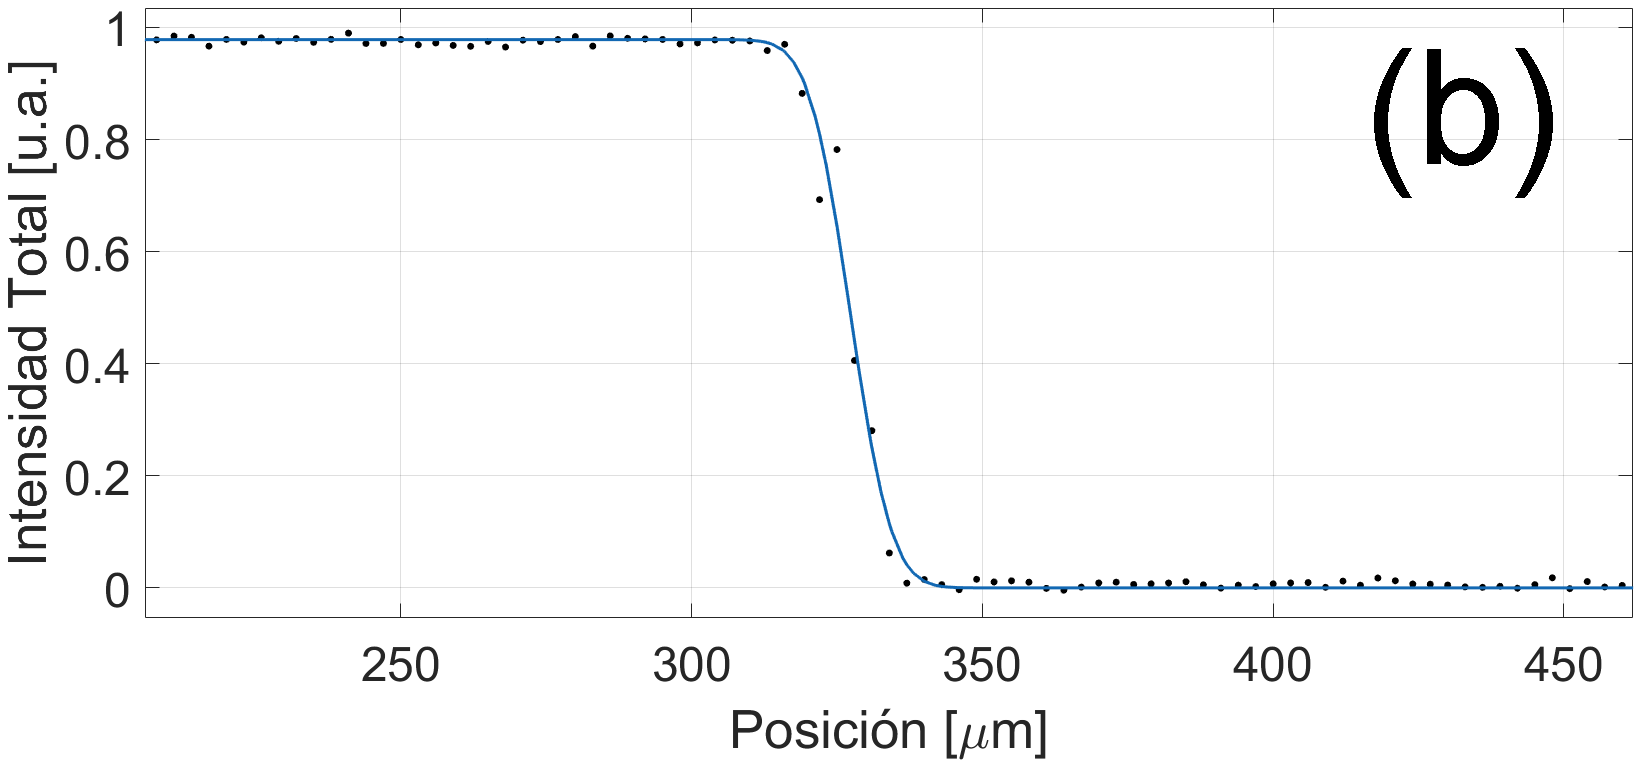
\includegraphics[scale=0.25]{Figs/microespectrometro/goodresol.png}
\hfill%
\hfill%
\caption{(a) Barrido de 1000 $\mu m$ con paso de 1 micrón entre la banda pancromática y el cromo. La resolución espacial obtenida del ajuste fue igual a $(292 \pm 12)~ \mu m$. El $R^{2}$ del ajuste fue igual a 0.98. (b) Barrido de 500 $\mu m$ con paso de 1 micrón entre la banda pancromática y el cromo. La resolución espacial obtenida del ajuste fue igual a $(11 \pm 1)~ \mu m$. El $R^{2}$ del ajuste fue igual a 0.99.}
\label{fig:bgresol}
\end{figure}

Se obtuvo la resolución espacial del microespectrómetro para distintas distancias entre el objetivo y el filtro que fueron variadas girando manualmente la rosca del componente optomecánico \href{https://www.thorlabs.com/thorproduct.cfm?partnumber=SM1V15}{SM1V15} sobre el que se encontraba montado el objetivo a la hora de realizar esta mediciones que se muestran aquí, montaje que se muestra en la Figura \ref{fig:montajecirc}. 
\begin{figure}[H]
	\centering
	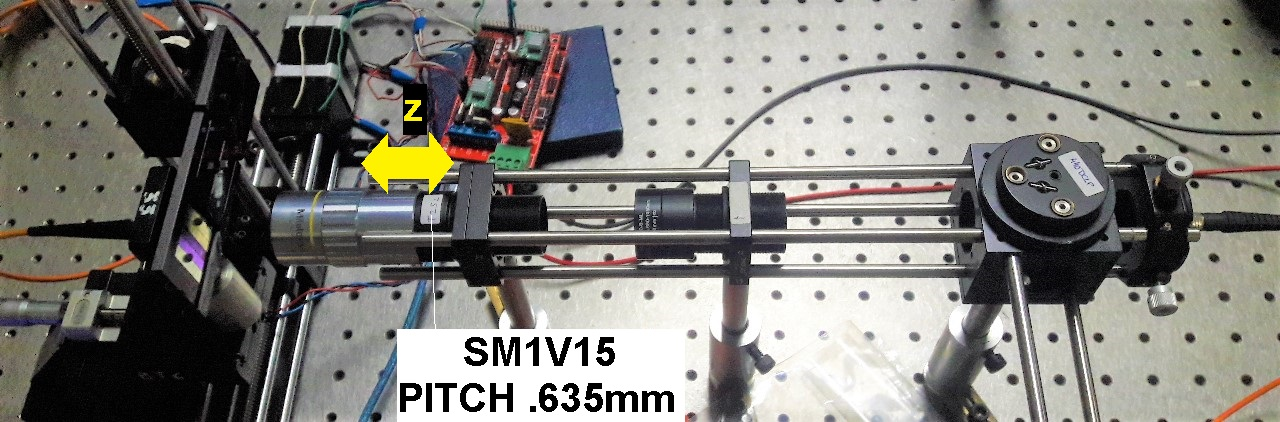
\includegraphics[width=1.0\textwidth]{Figs/microespectrometro/ajustefocoz.jpg}
	\caption{Girando manualmente la rosca del \href{https://www.thorlabs.com/thorproduct.cfm?partnumber=SM1V15}{SM1V15} se varió la distancia entre el objetivo y el filtro, para modificar el foco. El $\textit{pitch}$ del SM1V15 es igual a 0.635 mm y es igual a la distancia lineal que avanza el objetivo por cada revolución completa del componente.}
	\label{fig:montajecirc}
\end{figure}

Para cada distancia entre el objetivo y el filtro se obtuvo la resolución espacial a partir del ajuste de las mediciones y se graficó dicha resolución en función de la distancia variada con el SM1V15, como se muestra en la Figura \ref{fig:resolespz}. Se colocó el origen de coordenadas del eje $\textit{z}$, del eje óptico, en el mínimo de la resolución espacial obtenida. 

\begin{figure}[H]
	\centering
	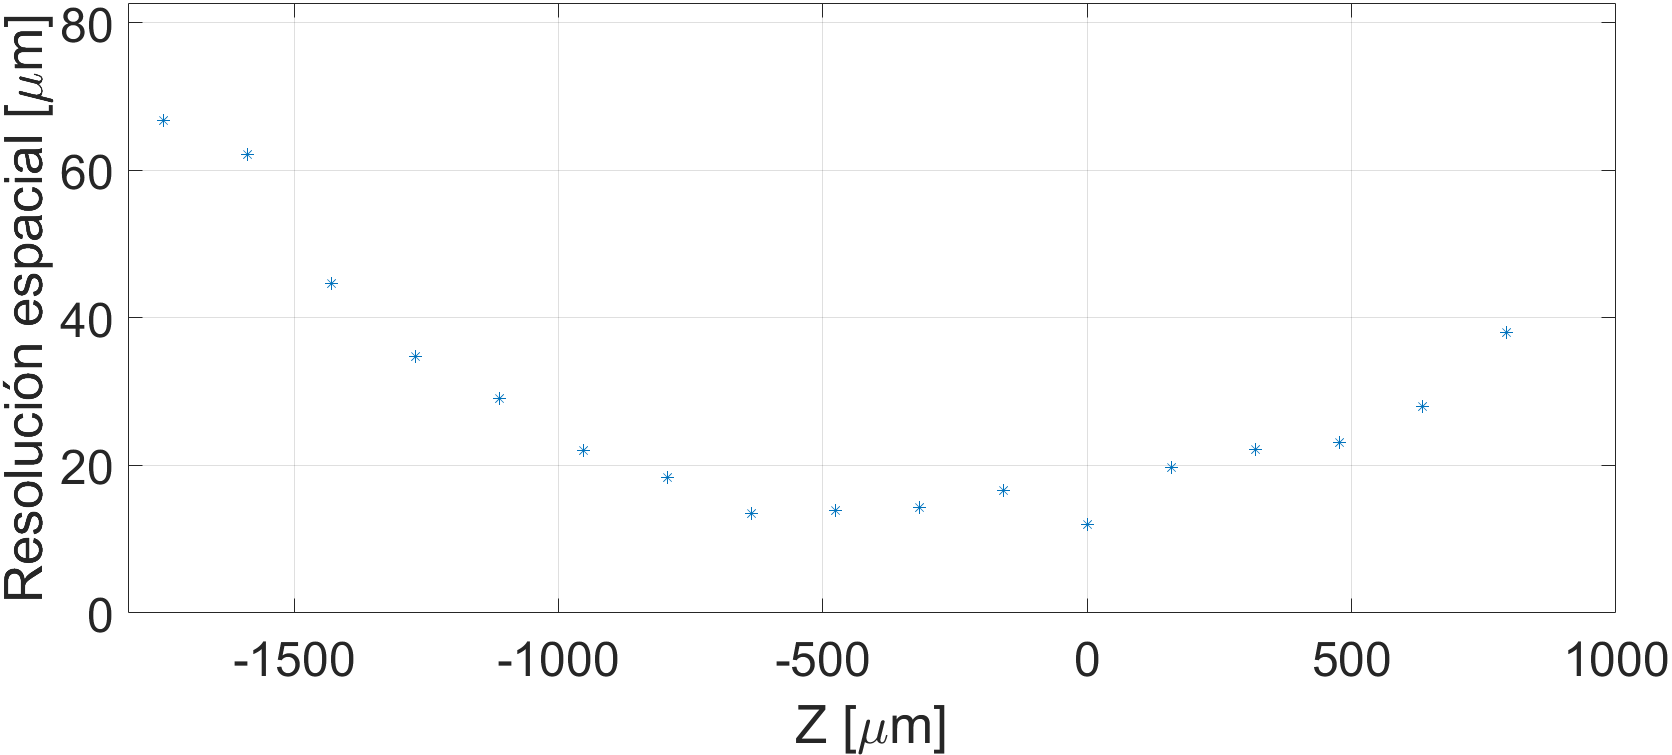
\includegraphics[width=1.0\textwidth]{Figs/microespectrometro/focoz.png}
	\caption{Gráfico de la resolución espacial en función de la distancia entre el filtro y el objetivo variada con el SM1V15.}
	\label{fig:resolespz}
\end{figure}

A partir de la determinación experimental del gráfico de la Figura \ref{fig:resolespz}, se decidió modificar el SM1V15 sobre el que se encontraba montado el objetivo por el componente \href{https://www.thorlabs.com/thorProduct.cfm?partNumber=SM1Z#ad-image-0}{SM1Z} (Ver Figura \ref{fig:micromfinal}). Se le encontraron dos desventajas al SM1V15 que afectaron la calidad de las mediciones. En primer lugar, el montaje del SM1V15 sobre el \textit{cage} del microespectrómetro hace que el objetivo no mantenga una estabilidad en la altura respecto del eje óptico, ya que luego de cada variación de la distancia entre el objetivo y el filtro, se debe asegurar el SM1V15 con un anillo y eso repercute en la alineación del sistema. Esta desventaja es superada por el montaje con el SM1Z ya que la distancia entre el objetivo y el filtro se realiza con una perilla micrométrica, por lo que la altura del objetivo permanece estable y alineada. En segundo lugar, el SM1V15 tiene un \textit{pitch} de 0.635 mm, es decir por cada revolución completa realiza un desplazamiento de 0.635 mm y se puede subdividir ese desplazamiento en fracciones de vuelta de forma arbitraria manualmente y en consecuencia de forma imprecisa. Un método de medición del ángulo rotado debería ser implementado, con su propia incertidumbre. Esta desventaja también fue superada por el montaje con el SM1Z que tiene un \textit{pitch} de 50 $\mu m$, con un paso mínimo de 1 $\mu m$ que se puede apreciar en la escala del tornillo micrométrico con el que se realiza la variación de la distancia. 

La resolución espacial del microespectrómetro estimada teóricamente está limitada por la difracción, de acuerdo al criterio de Rayleigh pero tiene una cota superior que es el tamaño del diámetro del \textit{core} de la fibra óptica multimodo acoplada al espectrómetro \cite{turrell}. Esta sentencia tan importante se puede justificar por el hecho de que se puede pensar el \textit{core} de la fibra como un \textit{pinhole} de un microscopio `pseudo-confocal', pues el detector tiene un área sensible mayor a la requerida para poder obtener la resolución óptica de dicho tipo de microscopio. Más aún, esto fue corroborado experimentalmente lo que demuestra la validez de dicha hipótesis teórica.

De acuerdo al criterio de Rayleigh, la resolución estimada teóricamente del microespectrómetro, limitada por difracción, debería variar entre los 0.98 $\mu m$ (si $\lambda = 450 ~nm$) y los 1.96 $\mu m$ (si $\lambda = 900 ~nm$), de acuerdo a las longitudes de onda empleadas con este equipo. Con la magnificación del microespectrómetro igual a 10X, la dimensión de las imágenes de los objetos de dicha resolución deberían ser de entre los 9.8 $\mu m$ y los 19.6 $\mu m$. Para poder muestrear correctamente dichas imágenes sin pérdida de resolución del objetivo, de acuerdo al Teorema de Nyquist-Shannon, se debería utilizar un detector con un área sensible de diámetro igual a la mitad del valor de dichas imágenes, es decir debería tener un diámetro de entre 4.8 $\mu m$ y 9.8 $\mu m$. Estos diámetros aplican para cualquier tipo de detector, ya sea para el sensor CMOS de la cámara ó para el diámetro de la apertura del espectrómetro que viene dada por el diámetro del \textit{core} de la fibra óptica multimodo. En consecuencia, en lo que respecta a la resolución óptica limitada por difracción de acuerdo al criterio de Rayleigh, se hace notar que no aplica al caso del equipo aquí presentado, ya que se midió una resolución óptica del orden de los 10 $\mu m$ con el equipo puesto en foco para la banda pancromática que no se corresponde con la estimación de Rayleigh que es del orden de los 1.3 $\mu m$. Esto se debe a que el diámetro del \textit{core} de la fibra óptica multimodo es de 200 $\mu m$, unas 20 veces más grande del diámetro requerido por Nyquist. Más aún, la resolución obtenida no es la predicha por la resolución de un microscopio confocal que debería incluso mejorar la resolución de la estimación de Rayleigh. Esto es así pues el diámetro del \textit{core} de la fibra que actúa como \textit{pinhole} no cumple específicamente la condición de ser del tamaño del orden del límite del diámetro del disco de Airy de difracción \cite{wilson}. De esta manera, se tiene que con el diámetro del \textit{core} de la fibra óptica multimodo del espectrómetro no se aprovecha el poder de resolución del objetivo ni la confocalidad por el sólo hecho de que el \textit{core} de la fibra actúe como \textit{pinhole}. La solución a este problema sería utilizar una fibra óptica multimodo con el diámetro correcto estimado con el costo de aumentar los tiempos de integración de las mediciones y de disminuir la relación señal-ruido de las mismas.

Ahora bien, se consideró el \textit{core} de la fibra óptica como si fuera un sensor compuesto por un solo elemento fotosensible (`1 solo píxel´) cuyo diámetro igual a 200 $\mu m$ estableció el tamaño de la imagen y que a partir de considerar la magnificación del microespectrómetro de 10X, se estimó por óptica geométrica que el diámetro del objeto detectado sobre el filtro tenía que ser de 20 $\mu m$, resultado del cociente entre el tamaño de la imagen y de la magnificación. Esta estimación sí se cumple experimentalmente de acuerdo a los resultados obtenidos ya que el radio de dicho objeto estimado de 10 $\mu m$ se solapa con la resolución espacial obtenida en los barridos con el microespectrómetro puesto en foco.

Los resultados del gráfico de la Figura \ref{fig:resolespz} permitieron corroborar experimentalmente la estimación teórica de la resolución espacial y representó el punto de partida para la integración de la cámara al equipo para facilitar la puesta en foco del equipo y para tener un \textit{feedback} visual de la región que se estaba midiendo en tiempo real. Se hace notar que sin la integración de una cámara al equipo, la única respuesta que se tenía del microespectrómetro era la medición del espectro de transmisión que se materializaba en un gráfico de intensidad en función de la longitud de onda. Y, en particular al realizar las mediciones por transmisión la puesta en foco no resultó tan inmediata como sí lo es el caso de las mediciones por reflexión donde la curva de discriminación del foco le asigna una posición unívoca al objetivo respecto de la superficie que se quiere adquirir a partir de la determinación del máximo de la intensidad reflejada (Ver \cite{mour}, Fig. 4). 

\singlespacing
\subsection{Puesta en foco de la cámara y \textit{mapeo} del espectrómetro con la cámara}
\label{sec:fococam}
\spacing{1.5}

\hspace{0.5cm}Luego de poner en foco el microespectrómetro, es decir luego de determinar el mínimo de la resolución espacial medida, se puso en foco la cámara, como se indicó en el diagrama de flujo de la Figura \ref{fig:diagpuestfoc}. Para ello, utilizando la interfaz gráfica desarrollada para adquirir simultáneamente en vivo la imagen de la cámara y la medición del espectrómetro, se visualizó la imagen de la cámara y modificando manualmente la posición de la cámara en el eje óptico a partir del deslizamiento del \textit{cage} sobre las barras de acero (Ver Figura \ref{fig:modmanualcam}), se fijó dicha distancia al observar una imagen nítida. Dicha distancia es la distancia que se denota con la letra B en la imagen de  la Figura \ref{fig:modmanualcam} y es la distancia en el eje óptico entre la cámara y el centro del beamsplitter que se encontraba montado sobre el cubo optomecánico \href{https://www.thorlabs.com/thorproduct.cfm?partnumber=C6W}{C6W}. Al mismo tiempo la distancia B debería coincidir con la distancia de la fibra óptica respecto del beamsplitter, denominada A, de forma tal de que ambos detectores tengan la misma magnificación, ya que fueron colocados a la distancia focal de la lente de tubo.  

\begin{figure}[H]
	\centering
	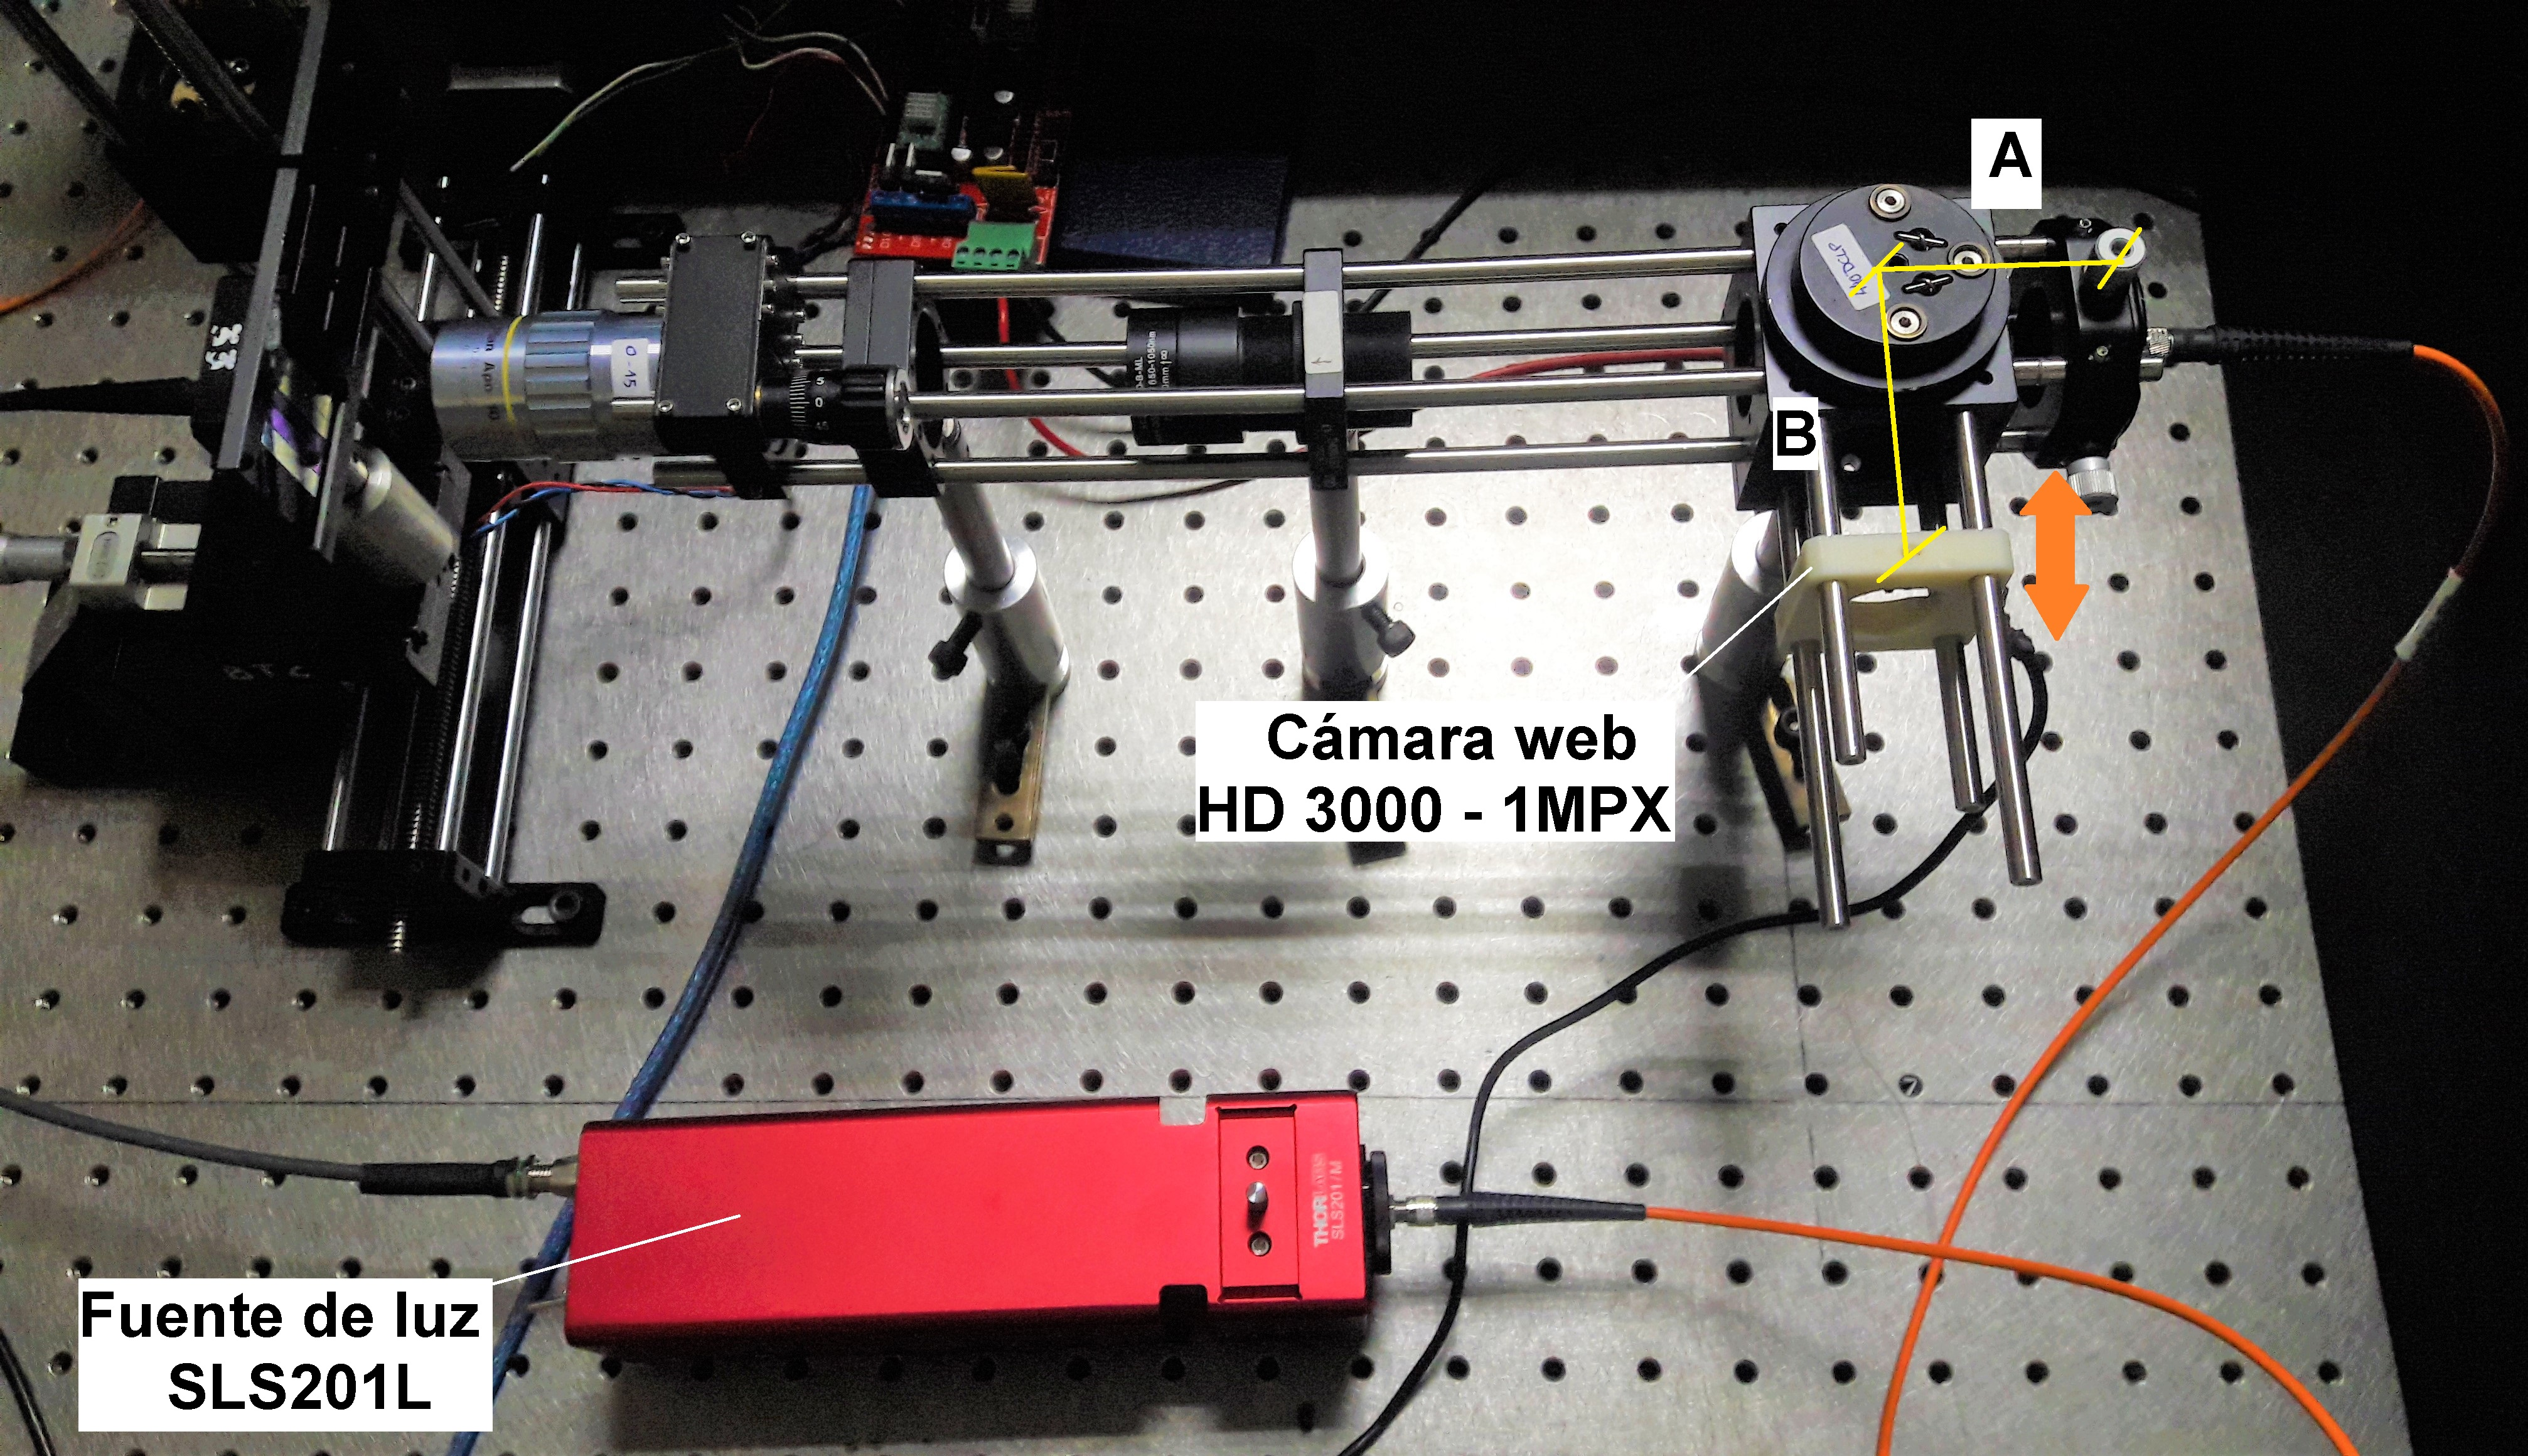
\includegraphics[width=1.0\textwidth]{Figs/microespectrometro/mapespeccam.jpg}
	\caption{\textit{Setup} para \textit{mapear} el espectrómetro con la cámara.}
	\label{fig:modmanualcam}
\end{figure}

Luego de poner en foco la cámara se realizó el \textit{mapeo} de la región de medición del espectrómetro sobre la imagen de la adquisición de la cámara \cite{frise}. Esto es, se identificó la región medida con el espectrómetro en la imagen de la cámara. El arreglo experimental para realizar el \textit{mapeo} y el diagrama del camino óptico del mismo se muestran en las Figuras \ref{fig:modmanualcam} y \ref{fig:caminmapp}. Como se indicó anteriormente la fibra óptica de la fuente de luz era la misma que la fibra óptica acoplada al espectrómetro. Para realizar el \textit{mapeo} se conectó la fibra óptica montada sobre el \textit{cage} destinado a medir con el espectrómetro, a la fuente de luz. La fuente de luz divergente fue colimada por la lente de tubo y enfocada por el objetivo en la superficie exterior del filtro. La reflexión del haz de luz enfocado sobre el filtro atravesó el objetivo que colimó dicho haz y por medio de la lente de tubo y la reflexión en el \textit{beamsplitter} fue enfocado en la cámara.

\begin{figure}[H]
	\centering
	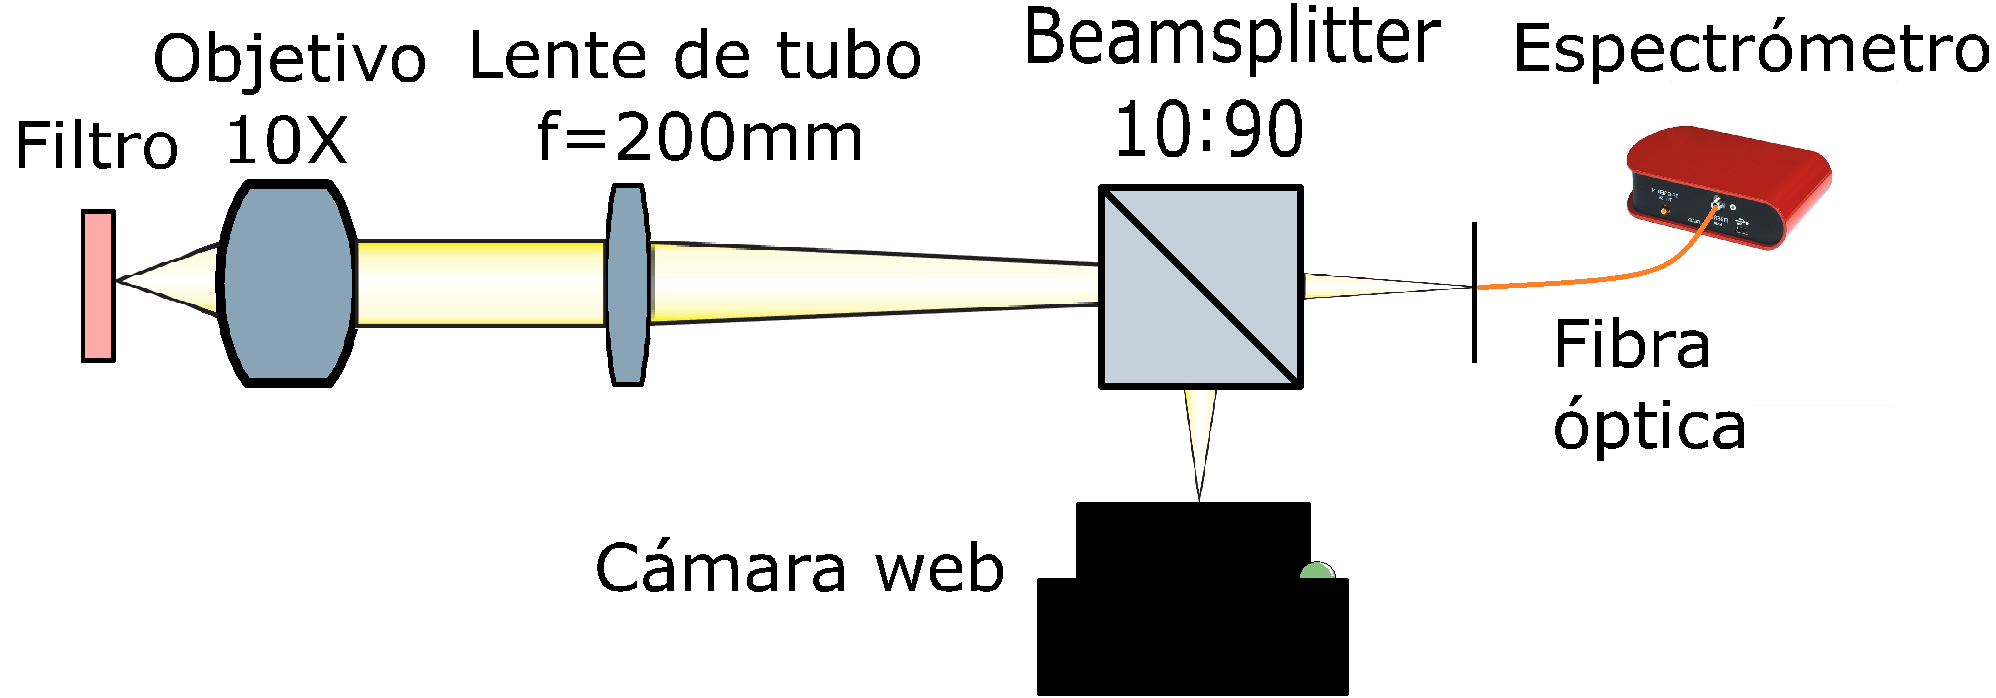
\includegraphics[width=1.0\textwidth]{Figs/microespectrometro/diagopticomapcamspec.png}
	\caption{Diagrama óptico del \textit{mapeo} del espectrómetro con la cámara.}
	\label{fig:caminmapp}
\end{figure}

 En la imagen de la Figura \ref{fig:refhazz} se muestra la visualización en la cámara de la posición en la imagen asociada a la reflexión del haz de luz enfocado sobre el filtro. Con los tornillos de la tapa de arriba del beamsplitter se ajustó la posición del beamsplitter para poder observar en el centro de la cámara la medición del espectrómetro, esto es para poder visualizar el haz reflejado en el centro de la imagen adquirida con la cámara. De esta manera se determinó que el centro de la imagen adquirida con la cámara estaba asociado con la medición efectiva del microespectrómetro.

Luego de realizar el \textit{mapeo}, el equipo quedó configurado de forma tal de tener un \textit{feedback} visual de la región de la medición realizada con el espectrómetro. Y, en adelante la región del filtro a medir a elección con el \textit{joystick} de la platina fue puesta en foco a partir de la visualización nítida de la imagen y de forma simultánea para la cámara y para el microespectrómetro, variando la distancia entre el objetivo y el filtro con la perilla micrométrica del SM1Z.

\begin{figure}[H]
	\centering
	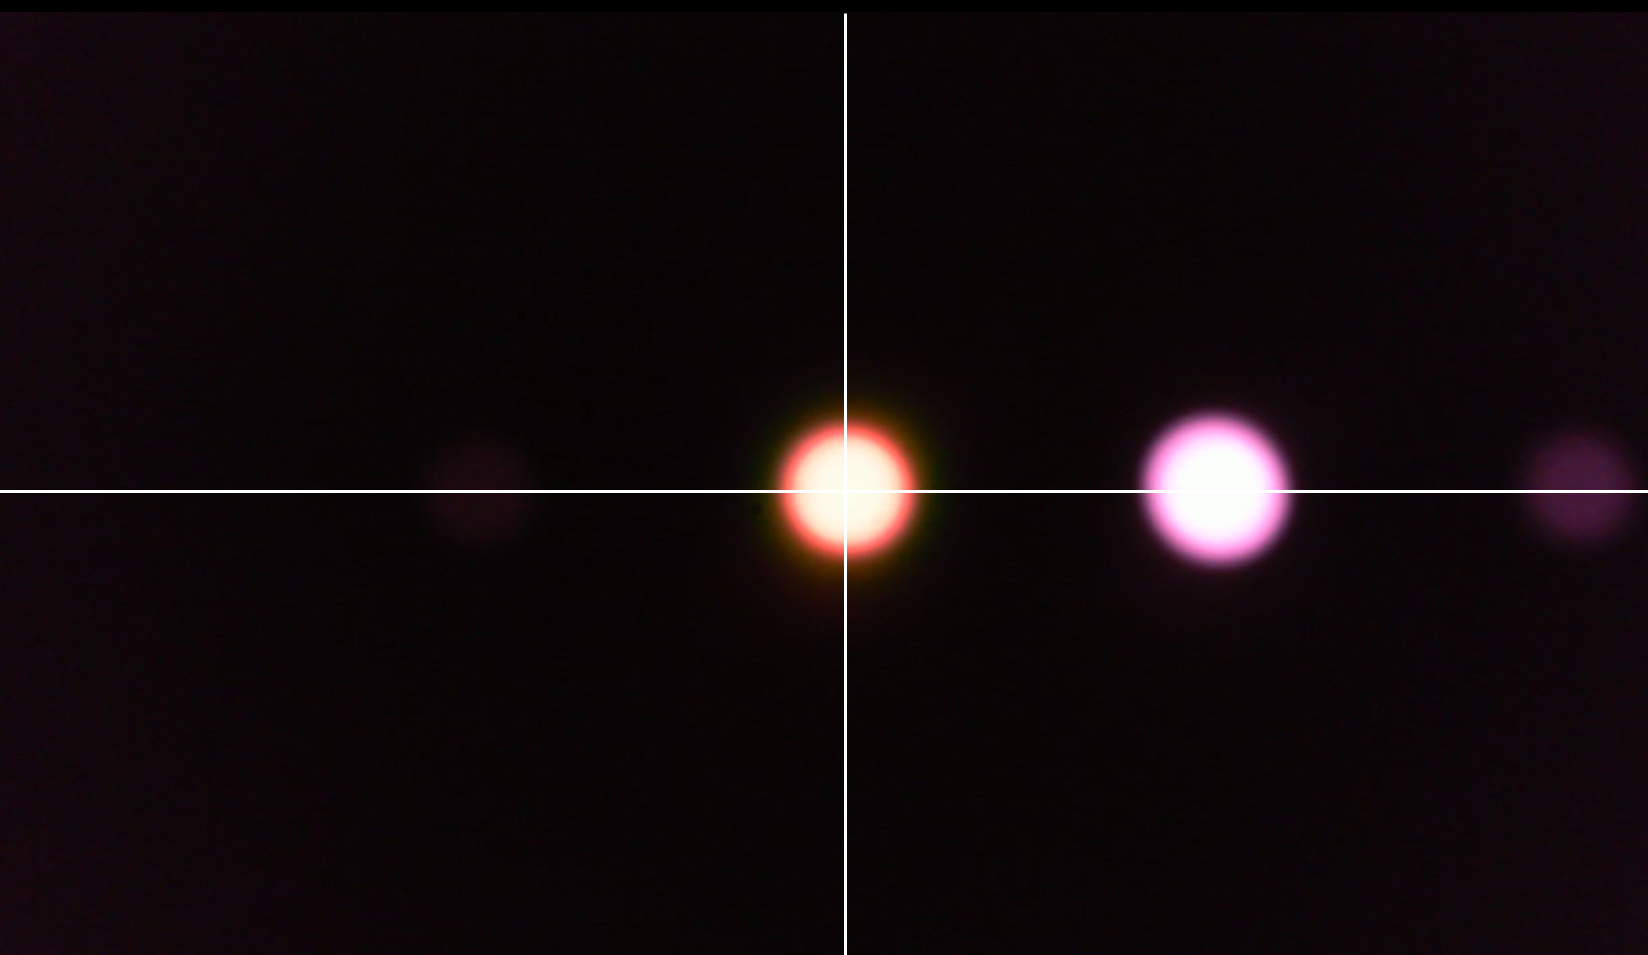
\includegraphics[scale=0.5]{Figs/microespectrometro/mapspectrometrocamera.png}
	\caption{Visualización en la cámara de la reflexión del haz de luz enfocado sobre el filtro.}
	\label{fig:refhazz}
\end{figure}


%%%%%%%%%%%%%%%%%%%%%%%%%%%%%%%%%%%%%%%%%%%%%%%%%%%%%%%%%%%%%%%%%%%%%%%%%%%%%%%%%%%%%%%%%%%%%%%%%%%%%%%%%%%%%%%%%%%%%%%%%%%%%%%%%%%%%%%%%%%%%%%%%%%%%%%%%%%%%%%%%%%%%%%%%%%%%%%%%%%%%%%%%%%%%%%%%%%%%%%%%%%%%%%%%%%%%%%%%%%%

\singlespacing
\section{Aplicación del microespectrómetro a la caracterización de filtros multiespectrales}
\label{sec:resgrales}
\spacing{1.5}

\hspace{0.5cm} En esta sección se muestran los resultados de la aplicación del microespectrómetro a la caracterización de filtros multiespectrales. Se describen los espectros de transmisión de cada banda del filtro [\ref{sec:espectransm}] que permitieron corrobar las características espectrales indicadas por el fabricante como la longitud de onda central de la banda (en inglés, \textit{CWL: center wavelength}) y el ancho espectral de la banda (en inglés, \textit{FWHM: Full Width Half Maximum}). Luego se realiza una caracterización de los espectros de transmisión de las manchas (Ver Figura \ref{fig:defectos} (b)) [\ref{sec:defctma}] y de los huecos (Ver Figura \ref{fig:defectos} (a)) [\ref{sec:defctag}].

%%%%%%%%%%%%%%%%%%%%%%%%%%%%%%%%%%%%%%%%%%%%%%%%%%%%%%%%%%%%%%%%%%%%%%%%%%%%%%%%%%%%%%%%%%%%%%%%%%%%%%%%%%%%%%%%%%%%%%%%%%%%%%%%%%%%%%%%%%%%%%%%%%%%%%%%%%%%%%%%%%%%%%%%%%%%%%%%%%%%%%%%%%%%%%%%%%%%%%%%%%%%%%%%%%%%%%%%%%%%

\singlespacing
\subsection{Espectro de transmisión de cada banda del filtro \href{https://github.com/jrr1984/open_frame_XYStage/blob/master/plot_spectrum_bands/plot_spectrum_bands.py}{\faGithub$_{3.4.1}$}}
\label{sec:espectransm}
\spacing{1.5}

\hspace{0.5cm}En esta sección se explica el procedimiento general realizado para medir el espectro de transmisión de cada una de las bandas espectrales del filtro. Luego de poner en foco el microespectrómetro, con el \textit{joystick} de la platina se desplazó al filtro para adquirir el espectro de cada una de sus bandas. Para eliminar el ruido de fotones propio del sensor del CCD del espectrómetro y otras fuentes de luz del laboratorio, se debe adquirir una medición con la fuente de luz que incide sobre el filtro apagada y con todas las luces del laboratorio apagadas además de recubir el equipo con la cartulina \textit{foam} negra. Dicho ruido de fondo puede ser luego eliminado de las mediciones del espectro de las bandas del filtro, o bien incluyéndolo como argumento del método \textit{take\_data}, \textit{use\_background}, del \textit{driver} de control del espectrómetro (\href{https://github.com/jrr1984/open\_frame\_XYStage/blob/master/XYStageAndSpec.py}{\faGithub$_{3.4.1.2}$}) ó bien tomando la diferencia entre el espectro de la banda medido y el ruido de fondo adquirido.

Para obtener el espectro de transmisión de cada banda se debe normalizar cada medición con el espectro de la fuente de luz utilizada, habiendo empleado los mismos tiempos de integración. La normalización es implementada realizando el cociente entre la medición del espectro de una banda y el espectro de la fuente de luz. Al mismo tiempo, las mediciones del espectro de cada banda deben ser realizadas con una buena relación señal-ruido.

En las Figuras \ref{fig:bnir}, \ref{fig:broja}, \ref{fig:bpanc}, \ref{fig:bverde} y \ref{fig:bazul} se muestran los espectros de transmisión de las bandas NIR, roja, pancromática, verde y azul del filtro respectivamente. Al mismo tiempo en la Figura \ref{fig:batod} se muestran los espectros de todas las bandas superpuestos a excepción de la banda pancromática.
\begin{figure}[H]
	\centering
	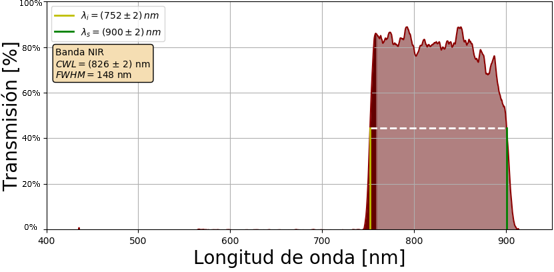
\includegraphics[scale=0.8]{Figs/microespectrometro/espectro_nirt.png}
	\caption{Espectro de transmisión de la banda NIR. Tiempo de integración de la luz: 10 ms.}
	\label{fig:bnir}
\end{figure}
\begin{figure}[H]
	\centering
	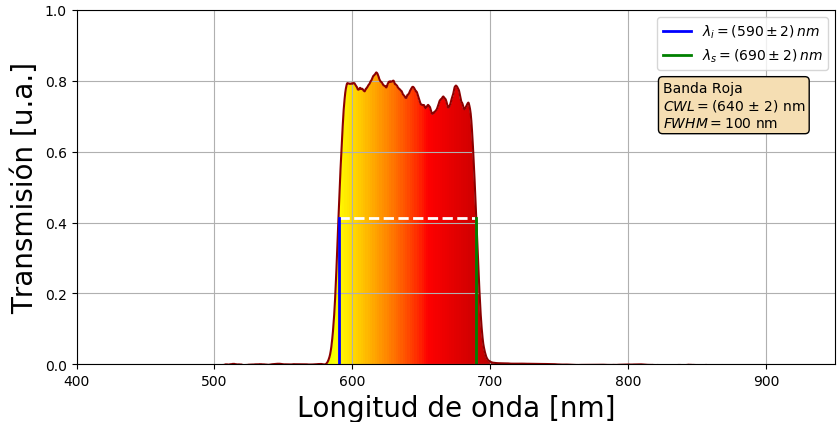
\includegraphics[scale=0.8]{Figs/microespectrometro/espectro_rojat.png}
	\caption{Espectro de transmisión de la banda roja. Tiempo de integración de la luz: 5 ms.}
	\label{fig:broja}
\end{figure}
\begin{figure}[H]
	\centering
	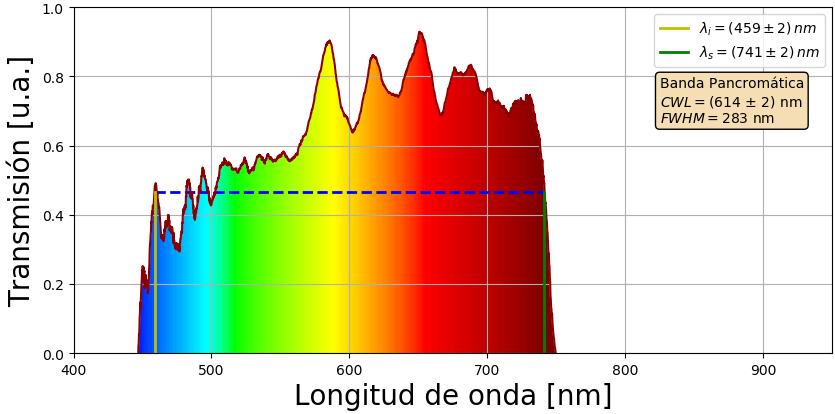
\includegraphics[scale=0.8]{Figs/microespectrometro/espectro_pancromaticat.png}
	\caption{Espectro de transmisión de la banda pancromática. Tiempo de integración de la luz: 2 ms.}
	\label{fig:bpanc}
\end{figure}
\begin{figure}[H]
	\centering
	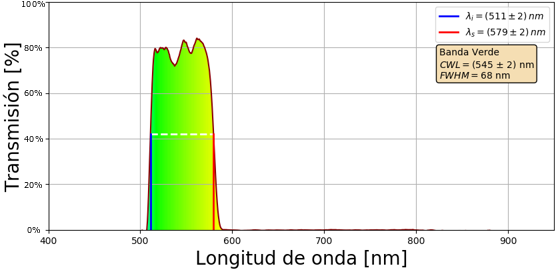
\includegraphics[scale=0.8]{Figs/microespectrometro/espectro_verdet.png}
	\caption{Espectro de transmisión de la banda verde.Tiempo de integración de la luz: 5 ms.}
	\label{fig:bverde}
\end{figure}
\begin{figure}[H]
	\centering
	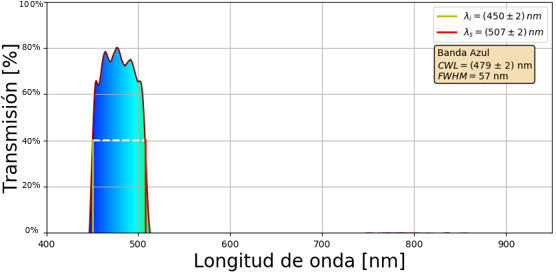
\includegraphics[scale=0.8]{Figs/microespectrometro/espectro_azult.png}
	\caption{Espectro de transmisión de la banda azul. Tiempo de integración de la luz: 20 ms.}
	\label{fig:bazul}
\end{figure}

 \begin{figure}[H]
	\centering
	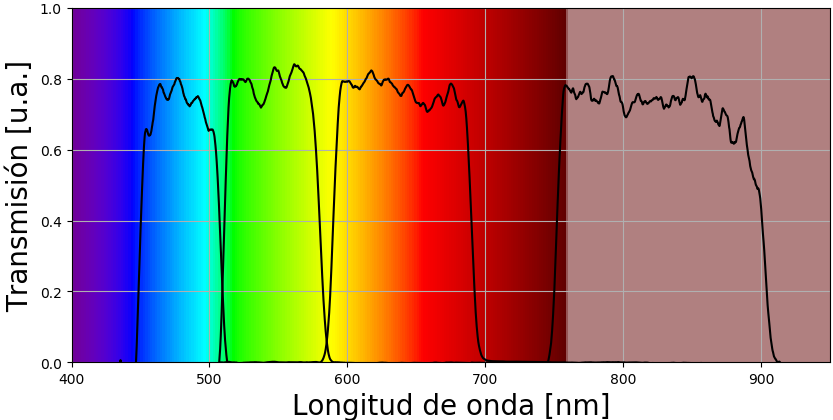
\includegraphics[scale=0.8]{Figs/microespectrometro/4bandas_conimshowT.png}
	\caption{Espectro de transmisión de todas las bandas a excepción de la banda pancromática.}
	\label{fig:batod}
\end{figure}

En la Tabla \ref{tabespc} se resumen los resultados de las características espectrales de cada banda. La columna  $|$FWHM $|$ indica el \textit{Full Width Half Maximum} (ancho de banda, ancho del rango de longitudes de onda comprendidas entre el valor de la mitad del máximo de transmisión). La columna $|$CWL$|$ indica la longitud de onda central de cada banda, asociada al punto medio del \textit{FWHM}. Las columnas $|$$\lambda_{i}$$|$, $|$$\lambda_{s}$$|$ indican el valor de la longitud de onda de corte inferior y superior, asociadas a los valores de longitud de onda de los extremos inferior y superior del rango del FWHM, respectivamente. Las incertezas de los valores reportados fueron de 2 nm en todos los casos.

 \begin{table}[H]
\begin{center}
\begin{tabular}{ |c|c|c|c|c| }    \toprule
Banda & CWL & FWHM & $\lambda_{i}$ & $\lambda_{s}$\\\midrule
\rowcolor{blue!15} Azul    & 479 nm & 57 nm & 450 nm & 507 nm  \\ 
\rowcolor{green!50} Verde  & 545 nm & 68 nm & 511 nm & 579 nm\\ 
Pancromática& 614 nm & 283 nm & 459 nm & 741 nm\\
\rowcolor{red!50} Roja & 640 nm & 100 nm  & 590 nm  & 690 nm\\
\rowcolor{maroon!20} NIR & 826 nm & 148 nm  &  752 nm & 900 nm\\
\bottomrule
 \hline
\end{tabular}
\end{center}
 \captionof{table}{Tabla de las especificaciones espectrales de cada banda del filtro.}
 \label{tabespc}
 \end{table}
De la comparación entre los valores de $\lambda_{i}$ y de $\lambda_{s}$ medidos y los reportados por el fabricante que indicó una incerteza del $1\%$, se hace notar que hay un solapamiento de los resultados de todas las bandas considerando las incertezas, a excepción de la banda pancromática donde la diferencia entre el valor medido y el reportado fue del $2\%$.
La medición de los espectros de transmisión de cada banda resultó fundamental para corroborar la capacidad de bloqueo de cada filtro de las longitudes de onda fuera del rango de valores comprendido por el \textit{FWHM}. Esto se vuelve más importante para el caso de filtros hiperespectrales que tienen cientos de bandas, cada una con un ancho espectral pasa banda de un cierto ancho, que permite extraer información específica y diferenciada.


%%%%%%%%%%%%%%%%%%%%%%%%%%%%%%%%%%%%%%%%%%%%%%%%%%%%%%%%%%%%%%%%%%%%%%%%%%%%%%%%%%%%%%%%%%%%%%%%%%%%%%%%%%%%%%%%%%%%%%%%%%%%%%%%%%%%%%%%%%%%%%%%%%%%%%%%%%%%%%%%%%%%%%%%%%%%%%%%%%%%%%%%%%%%%%%%%%%%%%%%%%%%%%%%%%%%%%%%%%%%

\singlespacing
\subsection{Caracterización espectral de las manchas}
\label{sec:defctma}
\spacing{1.5}

\hspace{0.5cm}Los resultados del algoritmo de detección de los defectos en las imágenes de microscopía adquiridas (Ver Sección \ref{sec:secalg}), permitieron determinar su tamaño, área, etc., pero no permitieron establecer si los defectos introducían modificaciones en el espectro de transmisión del filtro. Es decir, las imágenes de microscopía nos brindaron información de un valor de intensidad para cada posición ($\textit{x,y}$) de una cierta imagen de una región del filtro. Con el microespectrómetro se pudo obtener la misma y mayor información pues para cada posición del filtro además de su valor de intensidad que sería la suma de las intensidades detectadas para cada longitud de onda, se puede obtener el espectro de transmisión.

Con el objetivo de determinar las inhomogeneidades del filtro, se caracterizaron en primer lugar los defectos del tipo manchas  (Ver Figura \ref{fig:defectos} (b)). En la Figura \ref{fig:barinted} se muestra el barrido lineal realizado de 150 $\mu m$, con un paso de 1$\mu m$, desde la banda azul hasta el cromo atravesando un defecto de transmisión o mancha. En la imagen de la Figura \ref{fig:batod} se señala con un círculo blanco dicha mancha. Del ajuste de la transición entre la banda azul y el cromo se determinó que dicho barrido fue realizado con una resolución espacial de $(14 \pm 2)~\mu m$, resultado que no se solapa con el esperado teóricamente de 10 $\mu m$.

 \begin{figure}[H]
	\centering
	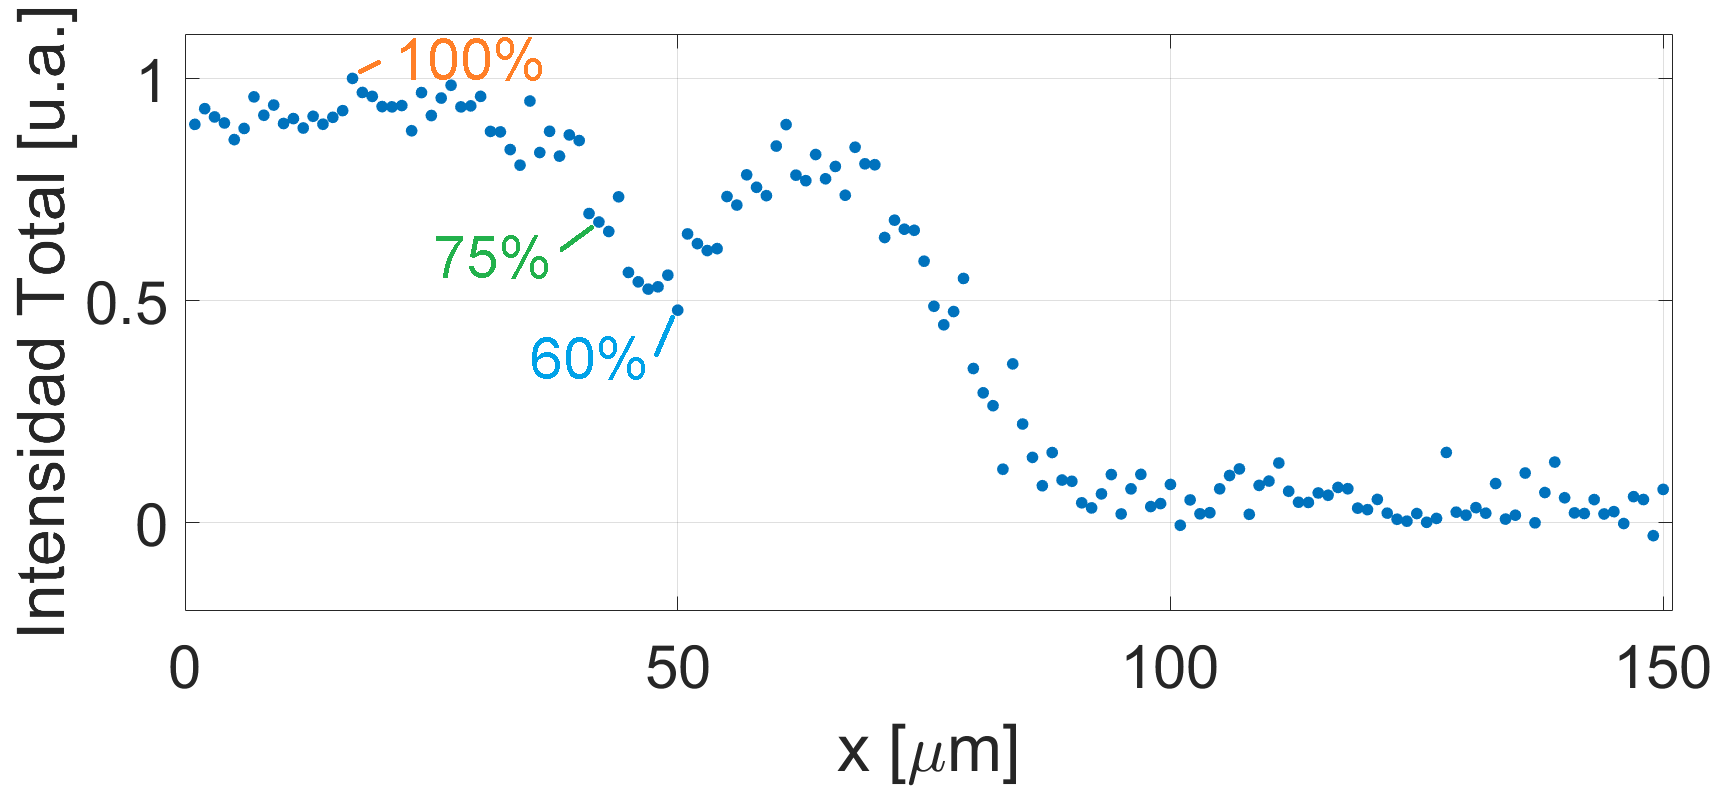
\includegraphics[width=1.0\textwidth]{Figs/microespectrometro/barridolamancha.png}
	\caption{Barrido lineal realizado de 150 $\mu m$, desde la banda azul hacia el cromo atravesando el defecto que se señala en la imagen.}
	\label{fig:barinted}
\end{figure}

 \begin{figure}[H]
	\centering
	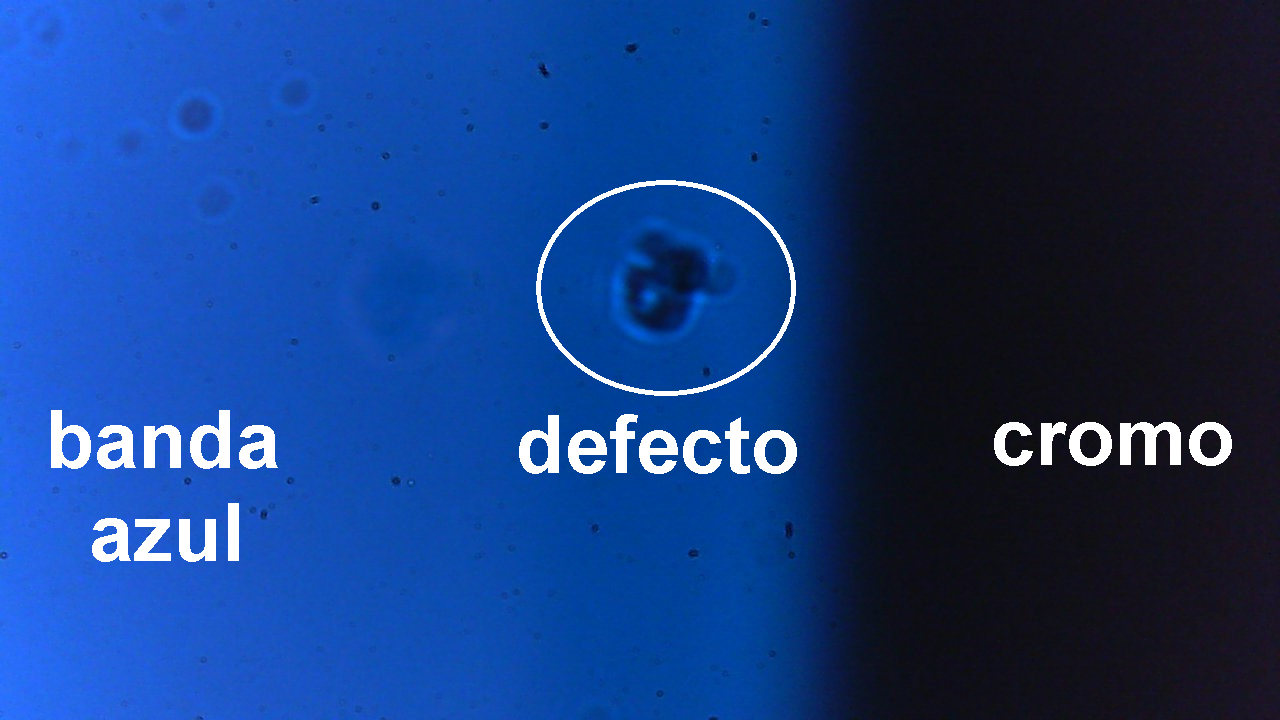
\includegraphics[scale=0.4]{Figs/microespectrometro/barridoenzdefecto.png}
	\caption{Imagen adquirida con la cámara asociada al barrido lineal realizado de 150 $\mu m$, desde la banda azul hacia el cromo atravesando un defecto de transmisión ó mancha que se señala en la imagen.}
	\label{fig:batod}
\end{figure}

En el gráfico de la Figura \ref{fig:merrmmin} se muestran tres espectros en simultáneo de los puntos señalados en el gráfico de la Figura \ref{fig:barinted}, para los casos del máximo de la suma de las intensidades detectadas dentro de la banda azul considerada la señal medida del 100\% de la transmisión de dicha banda, del 75\% y 60\% de la transmisión respecto de dicho máximo, respectivamente. Se hace notar que se determinó experimentalmente que este defecto de transmisión ó mancha no modifica la signatura espectral, es decir la forma funcional del espectro sino que produce una merma en la intensidad detectada en la banda, de acuerdo a la resolución espacial con la que fue medido. 

 \begin{figure}[H]
	\centering
	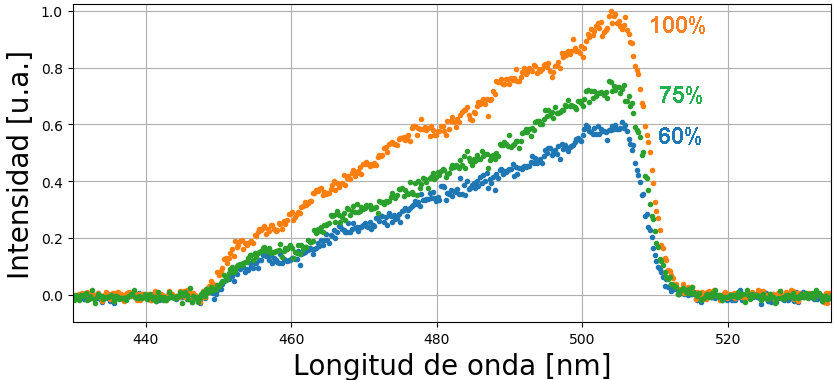
\includegraphics[width=1.0\textwidth]{Figs/microespectrometro/variacionintensidaddefecto.png}
	\caption{Gráficos de los espectros de transmisión superpuestos de los puntos del barrido señalados en la Figura \ref{fig:barinted}, asociados al máximo de intensidad del barrido detectado de la banda considerado el 100\% y al 75\% y 60\% de transmisión respecto de dicho máximo, respectivamente.}
	\label{fig:merrmmin}
\end{figure}

Se podría tomar como hipótesis para un futuro trabajo que las manchas influyen en las imágenes multiespectrales adquiridas con las cámaras satelitales de forma tal que los valores de intensidad de los píxeles de la cámara que estén en la misma posición que este tipo de defectos presentes en el filtro tendrían una merma en su valor original, produciendo una distorsión del espectro adquirido.


%%%%%%%%%%%%%%%%%%%%%%%%%%%%%%%%%%%%%%%%%%%%%%%%%%%%%%%%%%%%%%%%%%%%%%%%%%%%%%%%%%%%%%%%%%%%%%%%%%%%%%%%%%%%%%%%%%%%%%%%%%%%%%%%%%%%%%%%%%%%%%%%%%%%%%%%%%%%%%%%%%%%%%%%%%%%%%%%%%%%%%%%%%%%%%%%%%%%%%%%%%%%%%%%%%%%%%%%%%%%

\singlespacing
\subsection{Caracterización espectral de los huecos}
\label{sec:defctag}
\spacing{1.5}

\hspace{0.5cm}En esta última sección se muestran los resultados respecto de los espectros de transmisión de los huecos (Ver Figura \ref{fig:defectos} (a)). En particular, se muestran un barrido en dos dimensiones y un barrido lineal del hueco más grande del filtro (Ver \ref{fig:defectos} (a)) detectado en el Capítulo \ref{chap:zeiss}. Se ubicó dicho hueco a partir de la localización del mismo en las imágenes del \textit{tile scan} realizado en la banda azul. Con el \textit{joystick} de la platina desarrollada se posicionó el filtro con dicho hueco en el centro de la imagen adquirida con la cámara para medir su espectro de transmisión con el microespectrómetro.

En las Figuras \ref{fig:mapargbag} y \ref{fig:agujeroimg} (a) se muestran los resultados de una medición del espectro de transmisión de una región de 50 $\mu m$ x 50 $\mu m$, con pasos de 1 $\mu m$ en cada eje, dispuestos en un mapa de colores y un mapa de transmisión respectivamente\footnote{Se hace notar que la platina estaba siendo optimizada al momento de escribir esta tesis, a partir de la inclusión de rodamientos lineales LM6LUU en el eje \textit{$y$}. Del barrido en dos dimensiones que se muestra en las Figuras \ref{fig:mapargbag} y \ref{fig:agujeroimg} (a) se puede observar que la platina presenta problemas de repetibilidad de las posiciones, en el orden de los desplazamientos micrométricos.}. Estas mediciones podrían ser integradas a la interfaz gráfica de visualización desarrollada para facilitar su interpretación (Ver \ref{fig:GUI00}), ya que para cada píxel de la imágenes generadas se puede observar el espectro de transmisión correspondiente. En la Figura \ref{fig:agujeroimg} se muestra una imagen que fue adquirida con la cámara en simultáneo con la adquisición de los espectros de transmisión, donde se puede ver señalado con un círculo rojo el defecto tipo mancha que contiene a un hueco.

 \begin{figure}[H]
	\centering
	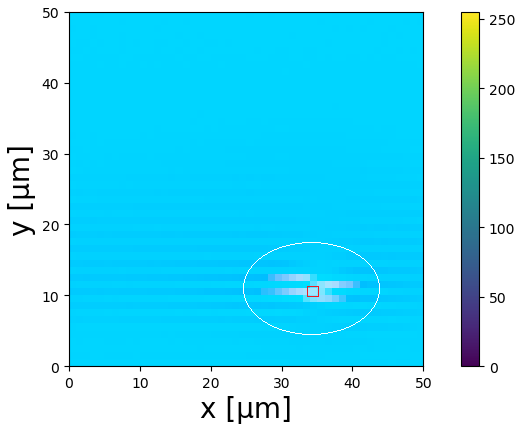
\includegraphics[scale=1.0]{Figs/microespectrometro/imhueco.png}
	\caption{Mapa de colores del espectro visible de una medición del espectro de transmisión de una región de 50 $\mu m$ x 50 $\mu m$.}
	\label{fig:mapargbag}
\end{figure}

El mapa de colores de la Figura \ref{fig:mapargbag} indica para cada píxel de la imagen que se generó, es decir para cada medición, el color asociado dentro del espectro visible. Se puede observar que el espectro de transmisión no es homogéneo en la región que contiene al hueco (señalada con el círculo blanco), ya que se observan píxeles de color blanco que deberían ser de color celeste. Al mismo tiempo se observan píxeles azules de mayor intensidad que están asociados a la mancha que recubre al hueco. 

En la Figura \ref{fig:agujeroimg} se muestra el mapa de transmisión de la región adquirida, que consiste de una imagen generada donde en cada píxel se representa el valor de la suma de las intensidades para cada longitud de onda de la medición asociada, normalizada con el máximo valor de dichos valores. Los píxeles negros del mapa de transmisión están asociados a la mancha que recubre al hueco que se observa en la imagen de la Figura \ref{fig:agujeroimg} (b).
 \begin{figure}[H]
%\centering
\hfill%
	\includegraphics[scale=1.0]{Figs/microespectrometro/tranhueco.png}
\hfill%
	\includegraphics[scale=0.6]{Figs/microespectrometro/imagujero.png}
	\hfill%
	\hfill%
	\caption{(a) Mapa de transmisión de una medición del espectro de transmisión de una región de 50 $\mu m$ x 50 $\mu m$. (b) Imagen de la banda azul que contiene al hueco caracterizado, adquirida con la cámara del equipo.}
	\label{fig:agujeroimg}
\end{figure}


En la Figura \ref{fig:perfilbacka} se muestra el perfil de intensidades asociados a los valores de la altura $\textit{y}$ = 11 $\mu m$ del mapa de transmisión de la Figura \ref{fig:agujeroimg} (a). El punto de dicho gráfico señalado con un círculo rojo está asociado unívocamente al píxel blanco recuadrado en rojo de la Figuras \ref{fig:mapargbag} y al píxel negro recuadrado en rojo de la Figura \ref{fig:agujeroimg} (a). Dicho punto asociado físicamente al hueco presenta una disminución de la intensidad transmitida del 64\%. El espectro de transmisión de este punto rojo se lo muestra en la Figura \ref{fig:espectbag} y se puede observar que además del espectro de transmisión esperado de la banda azul hay una fuerte componente espectral que contiene al rango de longitudes de onda de emisión de la fuente de luz. 

 \begin{figure}[H]
	\centering
	\includegraphics[width=1.0\textwidth]{Figs/microespectrometro/inten_totaldefecto.png}
	\caption{Perfil de intensidades asociados a los valores de la altura $\textit{y}$ = 11 $\mu m$ del mapa de transmisión de la Figura \ref{fig:agujeroimg} (a). Los puntos señalados con círculos están asociados a los espectros graficados en la Figura \ref{fig:esto}. En particular, el punto con un círculo rojo del centro del hueco, está vinculado a los píxeles recuadrados en rojo de las Figuras \ref{fig:mapargbag} y \ref{fig:agujeroimg} (a). }
	\label{fig:perfilbacka}
\end{figure}

\begin{figure}[H]
	\centering
\includegraphics[width=1.0\textwidth]{Figs/microespectrometro/espectroagback.png}
	\caption{Espectro de transmisión del centro del hueco, asociado al punto señalado con un círculo rojo en el gráfico de la Figura \ref{fig:perfilbacka} y a los píxeles recuadrados en rojo de las Figuras \ref{fig:mapargbag} y \ref{fig:agujeroimg} (a).}
\label{fig:espectbag}
\end{figure}

\begin{figure}[H]
%\centering
\hfill%
\includegraphics[scale=0.5]{Figs/microespectrometro/espectroshueco.png}
\hfill%
\includegraphics[scale=0.5]{Figs/microespectrometro/zoomdistorsionazul.png}
\hfill%
\hfill%
\caption{(a) Espectros de transmisión de los puntos señalados con un círculo de colores rojo, negro y celeste en la Figura \ref{fig:perfilbacka}. (b) \textit{Zoom} del espectro de transmisión para la región de longitudes de onda entre los 520 y los 890 nm.}
\label{fig:esto}
\end{figure}

Debido a la presencia de huecos el espectro de transmisión de la banda sufre una distorsión como se observa en los espectros de transmisión graficados en la Figura \ref{fig:esto} (a). Esto se puede ver en la Figura \ref{fig:esto} (b), donde se realizó un \textit{zoom} sobre la región de longitudes de onda comprendidas entre los 520 y los 890 nm. Se puede observar que el máximo de intensidad en dicha región espectral medido en el centro del hueco (espectro de color rojo) es aproximadamente 4 veces mayor que el máximo asociado al espectro medido en un punto del filtro que no contiene al hueco (espectro de color celeste). Este efecto podría repercutir en el espectro que se mida con la cámara multiespectral que utiliza filtros como el analizado en este trabajo. Es decir, los píxeles de la cámara multiespectral que se encuentren en la misma posición que los huecos del filtro podrían brindar información espectral errónea ya que siempre tendrían una contaminación del espectro de toda la luz que le ingrese a la cámara y no sólamente la luz del espectro de la banda asociada a los píxeles en cuestión. 

%Por último, se realizó un gráfico de la intensidad total transmitida en función de la posición del filtro análogo al de la Figura \ref{fig:perfilbacka}, pero se restringieron las intensidades medidas asociadas a la región espectral contenida entre los 520 y los 890 nm, como se muestra en la Figura \ref{fig:barrhueco}. De dicho gráfico se puede determinar que 

 %\begin{figure}[H]
%	\centering
%\includegraphics[width=1.0\textwidth]{Figs/microespectrometro/inbarrhueco.png}
	%\caption{Perfil de intensidades asociados a los valores de la altura $\textit{y}$ = 11 $\mu m$ del mapa de transmisión de la Figura \ref{fig:mapatransmag}, considerando las intensidades medidas asociadas a la región espectral contenida entre los 520 y los 890 nm. Los puntos señalados con círculos están asociados a los espectros graficados en las Figuras \ref{fig:esto} (a) y (b). En particular, el punto con un círculo rojo del centro del hueco, está vinculado a los píxeles recuadrados en rojo de las Figuras \ref{fig:mapargbag} y \ref{fig:mapatransmag}. }
%\label{fig:barrhueco}
%\end{figure}




